\documentclass[aps, prb, showpacs, twocolumn, notitlepage, superscriptaddress]{revtex4-1}
\usepackage{amsmath}
\usepackage{amssymb,amscd,bm,dsfont,wasysym,mathrsfs,latexsym,psfrag,accents,mathtools}
\usepackage{graphicx}
\usepackage{multirow}
\usepackage{dcolumn}
\usepackage{float}
\usepackage{color}
\usepackage{xcolor}
\usepackage{amsthm}
\usepackage{hyperref}
\usepackage{boldline}
\usepackage[normalem]{ulem}
\setlength{\intextsep}{10pt}
\setlength{\textfloatsep}{5pt}

%adjust height of rows in a table
\setlength\extrarowheight{2.5pt}

\newcolumntype{L}[1]{>{\raggedright\arraybackslash}p{#1}}
\newcolumntype{C}[1]{>{\centering\arraybackslash}p{#1}}
\newcolumntype{R}[1]{>{\raggedleft\arraybackslash}p{#1}}

%% ultimate commands
	
	% align environment
			\newcommand{\e}[1]{\begin{align}{#1}\end{align}}	
		
	% fraction
		\newcommand{\f}[2]{\frac{#1}{#2}}
		\newcommand{\tf}[2]{\tfrac{#1}{#2}}
		
	% partial differentiation
		\newcommand{\p}[2]{\frac{\partial #1}{\partial #2}}
		\newcommand{\pf}[3]{\frac{\partial #1}{\partial #2}\bigg|_{#3}}
		\newcommand{\pa}[1]{\partial_{#1}}
		
	% label equations/sections
		\newcommand{\la}[1]{\label{#1}}

	% refer to equation, section, figure, appendix
		\newcommand{\q}[1]{Eq.\ (\ref{#1})}
		\newcommand{\qq}[2]{Eqs.\ (\ref{#1}-\ref{#2})}
		\newcommand{\s}[1]{Sec.\ \ref{#1}}
		\newcommand{\fig}[1]{Fig.\ \ref{#1}}		
		\newcommand{\app}[1]{App.\ \ref{#1}}				
		\newcommand{\tab}[1]{Tab.\ \ref{#1}}
		\newcommand{\ocite}[1]{Ref.\ \onlinecite{#1}}
				
				
	% brackets
		\newcommand{\brac}[1]{\left(\;#1\;\right)}
		\newcommand{\sq}[1]{\left[\;#1\;\right]}
		\newcommand{\cu}[1]{\left\{\;#1\;\right\}}

	% insert words in equation environment

		\newcommand{\iwith}{\ins{with}}
		\newcommand{\where}{\ins{where}}		
		\newcommand{\iand}{\ins{and}}
		\newcommand{\ior}{\ins{or}}
		\newcommand{\ifor}{\ins{for}}
		\newcommand{\st}{\ins{s.t.}}
		
	% sign functions
		\newcommand{\sgn}{\text{sgn}}

	% equal, approximate, proportional signs, limits
		\newcommand{\eq}{=&\;}
		\newcommand{\condeq}[1]{\as \substack{\sma{#1}\\=}\as}
		\newcommand{\condprop}[1]{\as \substack{\sma{#1}\\ \propto}\as}
		\newcommand{\limit}[1]{\substack{\text{lim}\\#1}\as}		
		\newcommand{\appr}{\approx &\;}
		\newcommand{\prop}{\propto&\;}
	
	% mathbb symbols
		\newcommand{\R}{\mathbb{R}}
		\newcommand{\I}{\mathbb{I}}
		\newcommand{\C}{\mathbb{C}}
		\newcommand{\bbs}{\mathbb{S}}
		\newcommand{\bbt}{\mathbb{T}}
		
		
% plane wave
	\newcommand{\eikr}{e^{i\bk \cdot \br}}
	\newcommand{\eikR}{e^{i\bk \cdot \bR}}
	\newcommand{\emikr}{e^{-i\bk \cdot \br}}
	\newcommand{\emikR}{e^{-i\bk \cdot \bR}}	

% divergence,curl,laplacian
\newcommand{\diverge}{\nabla \cdot}
\newcommand{\curl}{\nabla \times}
\newcommand{\lap}{\nabla^2}
\newcommand{\nabr}{\nabla_{\boldsymbol{r}}}
\newcommand{\nabk}{\nabla_{\boldsymbol{k}}}
\newcommand{\nabkp}{\nabla_{\boldsymbol{k}'}}

%fundamental constants
\newcommand{\bohr}{\mu_{\sma{B}}}
\newcommand{\gfac}{g_{\sma{0}}}
\newcommand{\lmt}{l^{\mt}}
\newcommand{\lmf}{l^{\text{-}4}}
\newcommand{\lmo}{l^{\mo}}




% specific to geometric_orbital
\newcommand{\om}{orbital magnetization }
\newcommand{\omm}{orbital magnetization}
\newcommand{\zf}{Zilberman-Fischbeck }
\newcommand{\checkgp}{\check{g}^{\sma{\perp}}}
\newcommand{\bt}{$BT_{\sma{\perp}}$}
\newcommand{\bts}{$BT_{\sma{\perp}}$ }
\newcommand{\bise}{Bi$_2$Se$_3$}
\newcommand{\bises}{Bi$_2$Se$_3$ }



% c creation operators

\newcommand{\cdagk}{\dg{c}_{\bk}}
\newcommand{\ck}{\pdg{c}_{\bk}}
\newcommand{\cdagksig}{\dg{c}_{\bk,\sigma}}
\newcommand{\cksig}{\pdg{c}_{\bk,\sigma}}
\newcommand{\cdagkup}{c^\dagger_{\boldsymbol{k}\uparrow}}
\newcommand{\cdagkdo}{c^\dagger_{\boldsymbol{k}\downarrow}}
\newcommand{\ckup}{\pdg{c}_{\boldsymbol{k} \uparrow}}
\newcommand{\ckdo}{\pdg{c}_{\boldsymbol{k} \downarrow}}

\newcommand{\cdag}[1]{c^{\scriptscriptstyle{\dagger}}_{\scriptstyle{#1}}}
\newcommand{\cnod}[1]{c_{\scriptstyle{#1}}}


\newcommand{\cdj}{c^{\scriptscriptstyle{\dagger}}_{\scriptstyle{j \sigma}}}
\newcommand{\cnj}{c_{\scriptstyle{j' \sigma'}}}


% f creation operator

\newcommand{\fsig}{\pdg{f}_{\sigma}}
\newcommand{\fdagsig}{\dg{f}_{\sigma}}
\newcommand{\fup}{\pdg{f}_{\uparrow}}
\newcommand{\fdagup}{\dg{f}_{\uparrow}}
\newcommand{\fdo}{\pdg{f}_{\downarrow}}
\newcommand{\fdagdo}{\dg{f}_{\downarrow}}


%levi Cevita
\newcommand{\levi}[1]{\epsilon_{#1}}


%spin symbols
\newcommand\nup{\hat{n}_{f\uparrow}}
\newcommand\ndo{\hat{n}_{f\downarrow}}
\newcommand\avenup{{n}_{f\uparrow}}
\newcommand\avendo{{n}_{f\downarrow} }

% energies with varepsilon
\newcommand{\var}{\varepsilon}
%\newcommand{\var}[1]{\varepsilon_{#1}}
\newcommand{\efu}{\varepsilon_{\scriptscriptstyle{F}}^{\scriptscriptstyle{\uparrow}}}
\newcommand{\efd}{\varepsilon_{\scriptscriptstyle{F}}^{\scriptscriptstyle{\downarrow}}}
\newcommand{\ef}{\varepsilon_{\scriptscriptstyle{f}}}
\newcommand{\EF}{E_{\scriptscriptstyle{F}}}
\newcommand{\ek}{\varepsilon_{\boldsymbol{k}}}
\newcommand{\eF}{\varepsilon_{\scriptscriptstyle{F}}}
\newcommand{\enk}{\varepsilon_{n,\bk}}




% space

\newcommand\as{\;\;\;\;}
\newcommand\ass{\;\;\;\;\;\;\;\;}


\newcommand\Wline[2]{ \pdg{\W}_{\sma{#1 \leftarrow #2}}}


%hat operators

\newcommand{\hp}{\hat{p}}
\newcommand{\hbp}{\hat{\bp}}
\newcommand{\hbr}{\hat{\br}}
\newcommand{\hq}{\hat{q}}
\newcommand{\hH}{\hat{H}}
\newcommand{\hv}{\hat{\bv}}
\newcommand{\hx}{\hat{\bx}}
\newcommand{\hbpi}{\hat{\boldsymbol{\pi}}}
\newcommand{\hbPi}{\hat{\boldsymbol{\Pi}}}
\newcommand{\hPi}{\hat{{\Pi}}}



%bold symbols

\newcommand{\ba}{\boldsymbol{a}}
\newcommand{\bb}{\boldsymbol{b}}
\newcommand{\bc}{\boldsymbol{c}}
\newcommand{\bd}{\boldsymbol{d}}
\newcommand{\be}{\boldsymbol{e}}
\newcommand{\bff}{\boldsymbol{f}}
\newcommand{\bg}{\boldsymbol{g}}
\newcommand{\bh}{\boldsymbol{h}}
\newcommand{\bi}{\boldsymbol{i}}
\newcommand{\bj}{\boldsymbol{j}}
\newcommand{\bk}{\boldsymbol{k}}
\newcommand{\bkp}{\boldsymbol{k}^{{\sma{\perp}}}}
\newcommand{\bkone}{\boldsymbol{k_1}}
\newcommand{\bktwo}{\boldsymbol{k_2}}
\newcommand{\bp}{\boldsymbol{p}}
\newcommand{\bq}{\boldsymbol{q}}
\newcommand{\br}{\boldsymbol{r}}
\newcommand{\bs}{\boldsymbol{s}}
\newcommand{\bu}{\boldsymbol{u}}
\newcommand{\bv}{\boldsymbol{v}}
\newcommand{\bx}{\boldsymbol{x}}
\newcommand{\bz}{\boldsymbol{z}}
\newcommand{\bE}{\boldsymbol{E}}
\newcommand{\bA}{\boldsymbol{A}}
\newcommand{\bB}{\boldsymbol{B}}
\newcommand{\bC}{\boldsymbol{C}}
\newcommand{\bF}{\boldsymbol{F}}
\newcommand{\bG}{\boldsymbol{G}}
\newcommand{\bK}{\boldsymbol{K}}
\newcommand{\bM}{\boldsymbol{M}}
\newcommand{\bL}{\boldsymbol{L}}
\newcommand{\bO}{\boldsymbol{O}}
\newcommand{\bP}{\boldsymbol{P}}
\newcommand{\bQ}{\boldsymbol{Q}}
\newcommand{\bR}{\boldsymbol{R}}
\newcommand{\bS}{\boldsymbol{S}}
\newcommand{\bV}{\boldsymbol{V}}
\newcommand{\bze}{\boldsymbol{0}}
\newcommand{\bxi}{\boldsymbol{\xi}}
\newcommand{\bpi}{\boldsymbol{\pi}}
\newcommand{\bPi}{\boldsymbol{\Pi}}
\newcommand{\bomega}{\boldsymbol{\omega}}
\newcommand{\bsigma}{\boldsymbol{\sigma}}
\newcommand{\bcalf}{\boldsymbol{\calf}}
\newcommand{\bdelta}{\boldsymbol{\delta}}
\newcommand{\bkappa}{\boldsymbol{\kappa}}
\newcommand{\bmu}{\boldsymbol{\mu}}
\newcommand{\btau}{\boldsymbol{\tau}}
\newcommand{\bdeltapar}{\boldsymbol{\delta}_{\sma{\parallel}}}

%\mathfrak
\newcommand{\frake}{\mathfrak{e}}
\newcommand{\frako}{\mathfrak{o}}
\newcommand{\frakt}{\mathfrak{t}}
\newcommand{\fraks}{\mathfrak{s}}
\newcommand{\frakr}{\mathfrak{r}}
\newcommand{\mx}{\mathfrak{X}}
\newcommand{\mxx}{\mathfrak{X}^x}
\newcommand{\mxy}{\mathfrak{X}^y}
\newcommand{\bmx}{\boldsymbol{\mathfrak{X}}}


\newcommand{\orb}{\boldsymbol{\mathfrak{A}}}
\newcommand{\lutt}{\boldsymbol{\mathfrak{L}}}



%tilde
\newcommand{\tbPi}{\tilde{\bPi}}
\newcommand{\tPi}{\tilde{\Pi}}
\newcommand{\tbv}{\tilde{\bv}}
\newcommand{\tv}{\tilde{v}}
\newcommand{\tbmx}{\tilde{\bmx}}
\newcommand{\tmxx}{\tilde{\mx}^x}
\newcommand{\tmxy}{\tilde{\mx}^y}
\newcommand{\tmx}{\tilde{\mx}}
\newcommand{\tH}{\tilde{H}}
\newcommand{\tbsigma}{\tilde{\bsigma}}
\newcommand{\tsigma}{\tilde{\sigma}}
\newcommand{\tilu}[1]{\tilde{u}_{#1}}
\newcommand\tilX{\tilde{X}}
\newcommand\tilZ{\tilde{Z}}
\newcommand\tilGamma{\tilde{\Gamma}}
\newcommand\tilU{\tilde{U}}

%calligraphic
\newcommand{\calL}{{\cal L}}
\newcommand{\W}{{\cal W}}
\newcommand{\A}{{\cal A}}


% equal signs
\newcommand\kzeq{\;\stackrel{\mathclap{\normalfont\mbox{$\sma{\bar{k}_z}$}}}{=}\;}

%breve 
\newcommand{\breveg}{\breve{g}}


% symmetry operators
\newcommand{\inv}{\mathfrak{i}}
\newcommand{\mir}{\mathfrak{r}}
\newcommand\glide{\mathfrak{g}}
\newcommand\rot{\mathfrak{c}}
\newcommand\scr{\mathfrak{s}}
\newcommand\tra{\mathfrak{t}}


\newcommand{\calti}{{\cal T}_{\sma{\cal I}}}
\newcommand{\gdel}{g_{\boldsymbol{\delta}}}
\newcommand{\pgdel}{\pdg{g}_{\boldsymbol{\delta}}}
\newcommand{\bmz}{\bar{M}_z}
\newcommand{\calbmx}{{\cal \bar{M}}_x}
\newcommand{\calgdel}{\pdg{\breve{g}}_{\sma{\bdelta}}}
\newcommand{\brevegdel}{\pdg{\breve{g}}_{\sma{\bdelta}}}
\newcommand{\brevebmx}{\breve{\bar{M}}_x}
\newcommand{\uit}{U_{\sma{\cali T}}}
\newcommand{\utg}{U_{\sma{Tg \bdelta}}}
\newcommand{\ut}{U_{\sma{T}}}
\newcommand{\ug}{U_{\sma{g \bdelta}}}
\newcommand{\ubmx}{U_{\sma{\bmx}}}
\newcommand{\utbmz}{U_{\sma{T\bmz}}}
\newcommand{\calug}{\calg_{\sma{\bdelta}}}
\newcommand{\caluit}{\calu_{\sma{\cali T}}}
\newcommand{\caltgdel}{\breve{T}_{\sma{g \bdelta}}}
\newcommand{\brevetgdel}{\breve{T}_{\sma{g \bdelta}}}
\newcommand{\brevetbmx}{\breve{T}_{\sma{\bmx}}}
\newcommand{\hattbmx}{\hat{T}_{\sma{\bmx}}}
\newcommand{\brevetbmz}{\breve{T}_{\sma{\bmz}}}
\newcommand{\breveti}{\breve{T}_{\sma{\cali}}}
\newcommand{\caltbmz}{\calt_{\sma{\bmz}}}
\newcommand{\caltbmx}{\calt_{\sma{\bmx}}}
\newcommand{\calut}{\calu_{\sma{T}}}
\newcommand{\hatgdel}{\pdg{\hat{g}}_{\sma{\bdelta}}}
\newcommand{\hatTg}{\pdg{\hat{T}}_{\sma{g\bdelta}}}
\newcommand\csixdel{C_{\sma{6,\bdelta}}}
\newcommand\brevecsixdel{\breve{C}_{\sma{6,\bdelta}}}
\newcommand\cthreedel{C_{\sma{3,\bdelta}}}
\newcommand\brevecthreedel{\breve{C}_{\sma{3,\bdelta}}}
\newcommand\hatcthreedel{\hat{C}_{\sma{3,\bdelta}}}
\newcommand\cthreetwodel{C_{\sma{3,2\bdelta}}}
\newcommand\brevecthreetwodel{\breve{C}_{\sma{3,2\bdelta}}}
\newcommand\brevectwothreedel{\breve{C}_{\sma{2,3\bdelta}}}
\newcommand\ctwothreedel{C_{\sma{2,3\bdelta}}}
\newcommand\hatcsixdel{\hat{C}_{\sma{6,\bdelta}}}
\newcommand\ucsixdel{U_{\sma{C_6,\bdelta}}}
\newcommand\cndel{C_{\sma{n,\bdelta}}}
\newcommand\cbarndel{C_{\sma{\bar{n},\bdelta}}}
\newcommand\ucndel{U_{\sma{C_n,\bdelta}}}
\newcommand\hatcndel{\hat{C}_{\sma{n,\bdelta}}}
\newcommand\brevecndel{\breve{C}_{\sma{n,\bdelta}}}
\newcommand\brevectwotwodel{\breve{C}_{\sma{2,2\bdelta}}}
\newcommand\brevecfourdel{\breve{C}_{\sma{4,\bdelta}}}
\newcommand\brevectwodel{\breve{C}_{\sma{2,\bdelta}}}


% vectors and matrices
\newcommand{\vectwo}[2]{\begin{pmatrix} {#1}\\{#2} \end{pmatrix}}
\newcommand{\matrixtwo}[4]{\begin{pmatrix} #1 & #2 \\ #3 & #4 \end{pmatrix}}
\newcommand{\diagmatrix}[2]{\begin{pmatrix} #1 & 0 \\ 0 & #2 \end{pmatrix}}

% Pauli matrices
\newcommand{\szero}{\sigma_{\sma{0}}}
\newcommand{\sx}{\sigma_{\sma{1}}}
\newcommand{\sy}{\sigma_{\sma{2}}}
\newcommand{\sz}{\sigma_{\sma{3}}}
\newcommand{\tzero}{\tau_{\sma{0}}}
\newcommand{\tx}{\tau_{\sma{1}}}
\newcommand{\ty}{\tau_{\sma{2}}}
\newcommand{\tz}{\tau_{\sma{3}}}



% parafermion operators
\newcommand{\gt}{\gamma_{\sma{2}}}
\newcommand{\gth}{\gamma_{\sma{3}}}
\newcommand{\gfo}{\gamma_{\sma{4}}}
\newcommand{\gfi}{\gamma_{\sma{5}}}
\newcommand{\gj}{\gamma_{\sma{j}}}
\newcommand{\gtj}{\gamma_{\sma{2j}}}
\newcommand{\gtjpo}{\gamma_{\sma{2j+1}}}
\newcommand{\gtjpt}{\gamma_{\sma{2j+2}}}
\newcommand{\gtjmo}{\gamma_{\sma{2j-1}}}
\newcommand{\gtL}{\gamma_{\sma{2L}}}
\newcommand{\gtLpo}{\gamma_{\sma{2L+1}}}
\newcommand{\gtLpt}{\gamma_{\sma{2L+2}}}
\newcommand{\gtLmo}{\gamma_{\sma{2L-1}}}
\newcommand{\gtLmt}{\gamma_{\sma{2L-2}}}
\newcommand{\gtLmth}{\gamma_{\sma{2L-3}}}
\newcommand{\gtLmfo}{\gamma_{\sma{2L-4}}}


% insert text in equation
\newcommand{\ins}[1]{\;\;\;\;\text{#1}\;\;\;\;}


%momentum parallel and perpendicular
\newcommand{\kpar}{\boldsymbol{k}_{{\shortparallel}}}
\newcommand{\Dpar}{D^{g}_{{\shortparallel}}}
\newcommand{\kper}{k_{\perp}}


% Cnv 
\newcommand{\ctv}{C_{3v}}
\newcommand{\cfv}{C_{4v}}
\newcommand{\csv}{C_{6v}}
\newcommand{\cnv}{C_{nv}}


%C_n Time-reversal
\newcommand{\cnt}{C_n {\cal T}}
\newcommand{\cn}{C_n}
\newcommand{\cf}{C_4}
\newcommand{\cs}{C_6}
\newcommand{\ct}{C_3}
\newcommand{\cst}{C_6{\cal T}}
\newcommand{\cft}{C_4{\cal T}}
\newcommand{\ctt}{C_2{\cal T}}


% average 
\newcommand{\ave}[1]{\langle\,#1\,\rangle}



%inverse Angstroms and Angstroms
\newcommand{\invA}{\text{\AA^{\scriptscriptstyle{-1}}}}
\newcommand{\ang}{\text{\AA}}

% Lagrangian
\newcommand{\lag}{{\mathscr{L}}}


% green's function
\newcommand{\green}{{\mathscr{G}}}

% Cauchy principal value
\newcommand{\prin}{{\mathscr{P}}}

% imaginary and real parts
\newcommand{\imag}{{\mathscr{I}}}
\newcommand{\real}{{\mathscr{R}}}


%total differentiation
\newcommand{\totaldif}[2]{\frac{ d #1}{d #2}}

% Berry field
\newcommand{\cala}{{\cal A}}
\newcommand{\calb}{{\cal B}}
\newcommand{\calc}{{\cal C}}
\newcommand{\cald}{{\cal D}}
\newcommand{\cale}{{\cal E}}
\newcommand{\calf}{{\cal F}}
\newcommand{\calg}{{\cal G}}
\newcommand{\calh}{{\cal H}}
\newcommand{\tcalh}{\tilde{\cal H}}
\newcommand{\cali}{{\cal I}}
\newcommand{\calj}{{\cal J}}
\newcommand{\calk}{{\cal K}}
\newcommand{\call}{{\cal L}}
\newcommand{\calm}{{\cal M}}
\newcommand{\caln}{{\cal N}}
\newcommand{\calo}{{\cal O}}
\newcommand{\calp}{{\cal P}}
\newcommand{\calq}{{\cal Q}}
\newcommand{\calr}{{\cal R}}
\newcommand{\cals}{{\cal S}}
\newcommand{\calt}{{\cal T}}
\newcommand{\calu}{{\cal U}}
\newcommand{\calv}{{\cal V}}
\newcommand{\calw}{{\cal W}}
\newcommand{\calx}{{\cal X}}
\newcommand{\caly}{{\cal Y}}
\newcommand{\calz}{{\cal Z}}



%Gamma matrices
\newcommand{\gam}[1]{\Gamma_{#1}}

%determinant
\newcommand{\de}[1]{\text{det}[\;#1\;]}

%trace
\newcommand{\tr}[1]{\text{Tr}[\;#1\;]}




\newcommand{\noi}[1]{\noindent (#1)}
\newcommand{\imp}{\;\;\Rightarrow\;\;}
\newcommand{\mo}{\text{-}1}
\newcommand{\mt}{\text{-}2}
\newcommand{\minus}{\text{-}}
\newcommand{\oneover}[1]{\tfrac{1}{#1}}


% A command for inner product and bras and kets
\newcommand{\braket}[2]{\big\langle #1 \big| #2 \big\rangle}
\newcommand{\ketbra}[2]{\big|  #1  \big\rangle \big\langle #2 \big| }
\newcommand{\braopket}[3]{\big\langle #1 \big| #2 \big| #3 \big\rangle}
\newcommand{\bra}[1]{\big\langle#1\big|}
\newcommand{\ket}[1]{\big|#1\big\rangle}
\newcommand{\bigket}[1]{\bigl|#1\bigr\rangle}
\newcommand{\textket}[1]{|#1\rangle}

% Various bracketing commands
\newcommand{\of}[1]{\!\left(#1\right)}
\newcommand{\sqof}[1]{\left[#1\right]}
\newcommand{\cuof}[1]{\left\{#1\right\}}

% commutator and anticommutator
\newcommand{\comm}[2]{\left[#1,#2\right]}
\newcommand{\anticomm}[2]{\left\{#1,#2\right\}}
% sum on nearest neighbor bonds
\newcommand{\bond}{\left\langle i, j \right\rangle}
%\newcommand{\bondsum}{\sum_{\left\langle i, j \right\rangle}}
\newcommand{\nbond}{\left\langle\left\langle i, j \right\rangle\right\rangle}
% 1/2
\newcommand{\half}{\frac{1}{2} }
\newcommand{\thalf}{\tfrac{1}{2} }
% simplifies using the up and down arrows to denote spin
\newcommand{\up}{\uparrow}
\newcommand{\down}{\downarrow}
% Absolute value  
\newcommand{\abs}[1]{\left|#1\right|}

% Roman functions for real and imaginary parts
\newcommand{\re}{\mathrm{Re}}
\newcommand{\im}{\mathrm{Im}}


%Expectation values
\newcommand{\expect}[1]{\left\langle#1\right\rangle}
\newcommand{\pdag}{\phantom{\dagger}}
\newcommand{\pdg}[1]{{#1}^{\phantom{\dagger}}}

\newcommand{\bkap}{\bar{\glide}}
\newcommand{\bchi}{\bar{\chi}}
\newcommand{\baeta}{\bar{\eta}}
\newcommand{\lin}{\notag \\}
\newcommand{\ex}{\text{exp}}
\newcommand{\ab}{\alpha\beta}
\newcommand{\deli}{\Delta^{-1}}


\newcommand{\ra}{{R\,\alpha}}
\newcommand{\rax}{{R+\vec{x}\,\alpha}}

\newcommand{\rb}{{R'\,\beta}}
\newcommand{\rarb}{{R\,\alpha};R'\,\beta}
\newcommand{\zth}{\mathbb{Z}_3}


\newcommand{\xin}{x_{\tex{inv}}}
\newcommand{\low}{L$\ddot{\text{o}}$wdin\;}
\newcommand{\tex}[1]{\sma{\text{#1}}}











\newcommand{\kf}{k_{\scriptscriptstyle{F}}}

\newcommand{\bfk}{\boldsymbol{k}}
\newcommand{\bfq}{\boldsymbol{q}}



\newcommand{\bpm}{\begin{pmatrix}}
\newcommand{\epm}{\end{pmatrix}}
\newcommand{\nk}{n_{\boldsymbol{k}'}}
\newcommand{\dk}{\Delta_{\boldsymbol{k}'}}
\newcommand{\Dk}{\Delta_{\boldsymbol{k}}}
\newcommand{\tk}{\tilde{k}}
\newcommand{\tkp}{\tilde{k}'}
\newcommand{\bal}{\begin{align}}


\newcommand{\V}{V_{\text{eff}}}
\newcommand{\si}{\;\text{sin}\,}
\newcommand{\ta}{\;\text{tan}\,}
\newcommand{\co}{\;\text{\text{cos}}\,}
\newcommand{\te}{t_{\text{eff}}}
\newcommand{\ep}{\bar{\epsilon}}



\newcommand{\braa}[1]{\left\langle#1\right|_{\scriptscriptstyle{A}}}
\newcommand{\brab}[1]{\left\langle#1\right|_{\scriptscriptstyle{B}}}

\newcommand{\dg}[1]{#1^{\scriptstyle{\dagger}}}
\newcommand{\bof}[1]{\boldsymbol{#1}}
\newcommand{\sma}[1]{\scriptscriptstyle{#1}}
\newcommand{\po}{{\sma{+}} 1}



\newcommand{\noc}{n_{\sma{{occ}}}}
\newcommand{\ntot}{n_{\sma{{tot}}}}
\newcommand{\Z}{\mathbb{Z}}


\newcommand{\zpar}{Z_{\sma{\parallel}}}
\newcommand{\zper}{Z_{\sma{\perp}}}
\newcommand{\lper}{l_{\sma{\perp}}}
\newcommand{\bper}{B_{\sma{\perp}}}
\newcommand{\bpar}{B_{\sma{\parallel}}}

\newcommand{\order}{\text{O}}

% for review
\newcommand{\red}[1]{\textcolor{red}{#1}}
\newcommand{\blue}[1]{\textcolor{blue}{#1}}

% important quantities
\renewcommand{\H}{\mathcal{H}}
\newcommand{\barmu}{\bar{\mu}}
\newcommand{\barphi}{\bar{\varphi}}


\begin{document}

\title{Landau quantization of nearly degenerate bands}

\author{Chong Wang}\affiliation{Institute for Advanced Study, Tsinghua University, Beijing 100084, China}
\author{Wenhui Duan}\affiliation{Institute for Advanced Study, Tsinghua University, Beijing 100084, China}\affiliation{Department of Physics and State Key Laboratory of Low-Dimensional Quantum Physics, Tsinghua University, Beijing 100084, China}\affiliation{Collaborative Innovation Center of Quantum Matter, Tsinghua University, Beijing 100084, China}
\author{Leonid Glazman}\affiliation{
Department of Physics, Yale University, New Haven, Connecticut 06520, USA}
\author{A. Alexandradinata}\affiliation{
Department of Physics, Yale University, New Haven, Connecticut 06520, USA}

\begin{abstract}
\textbf{[abstract needs revamp]}
 In the semiclassical theory of Landau levels, a Bloch electron is driven by a magnetic field  along constant-energy band contours  (in quasimomentum space) known as orbits. We introduce a quantization rule for Landau levels of nearly degenerate orbits which are split by spin-orbit coupling. The average area $S$ of two spin-orbit-split orbits is assumed much larger than the difference in areas ($\delta S$), and also much larger than the inverse square of the magnetic length ($\lmt$). By treating both $\delta S/S$ and $1/l^2S$ as small parameters with finite ratio $l^2\delta S$, our perspective diverges from and generalizes previous semiclassical theories.  $l^2\delta S$ is the dimensionless measure of the field-induced hybridization between spin-orbit-split orbits; we allow for $l^2\delta S$ to be comparable with the Zeeman coupling. In the opposing regimes $l^2\delta S {{\ll}} 1$  and $l^2\delta S{\gg}1$, we recover the known Onsager-Lifshitz-Roth rules for nondegenerate and degenerate orbits, respectively.  In the absence of crystallographic symmetry, three real parameters are needed to tune a degeneracy between two Landau levels which have been split by the spin-orbit and Zeeman interactions. Here, we identify symmetry classes for which such degeneracies can be tuned by varying a single parameter, which might be the magnitude or orientation of the field, or a bias voltage in tunneling spectroscopy.  We demonstrate the utility of our rule for the Rashba 2DEG (for which an in-plane Zeeman field can induce a type-II Dirac point), Dresselhaus spin-orbit-coupled systems, and the angular magnetoresistance oscillations of semiconductor bilayer heterostructures.      
\end{abstract}
\date{\today}

% We demonstrate the utility of our rule for quasidegenerate orbits which  touch at isolated (type-II Dirac) points, as well as for orbits which (nearly) touch at \emph{all points} along their trajectory. In the former case, a wavepacket follows each spin-orbit-split orbit adiabatically, except at localized regions where quantum  tunneling (known as magnetic breakdown) is appreciable; in the latter case, adiabaticity is irrelevant and the orbits are completely reconstructed by the field.


%Magnetic breakdown is the phenomenon of quantum tunneling between semiclassical orbits; conventionally, the tunneling region is localized to \emph{isolated}  points   in momentum space, as exemplified by saddle- or Dirac points. Here, we introduce a qualitatively distinct form of tunneling that is delocalized over the entire orbit. Such nonlocal breakdown occurs wherever two orbits nearly touch at \emph{all points} along their trajectory, as exemplified in solids by the spin-orbit splitting of spin-degenerate energy bands. We formulate the Bohr-Sommerfeld quantization rules that are predictive of Landau levels in the presence of nonlocal breakdown. We propose the experimental signature to be an aperiodic beating in quantum oscillations of the magnetization or resistivity, which contrasts with the periodic beating that is well-known for two decoupled orbits.   

%By accounting for all dynamical and geometric phases induced by this spin-splitting, our work extends the known Onsager-Lifshitz-Roth rules for nondegenerate and degenerate orbits.


\maketitle

\section{Introduction}


%Semiclassical theory is predictive of Landau levels for solids in a weak magnetic field $B$. This theory has been extended to describe quantum tunneling between two orbits which intersect at \emph{isolated} points. Examples of such isolated points include saddle and type-II Dirac points, where tunneling respectively occurs between orbits of the same band (known as intraband magnetic breakdown) and between orbits of distinct bands (interband breakdown). As $B {\rightarrow} 0$, tunneling is localized to an arbitrarily small neighborhood of such isolated points, and occurs with half probability for the saddlepoint, and with unit probability for the  Dirac point.\footnote{If orbits nearly intersect, tunneling occurs with a probability that asymptotically $\sim e^{-c/B}$, where $c$ is field-independent;[Blount] as a  rule of thumb, this probability ${\sim} 1$ if the \emph{minimal} separation of the two orbits in $\bk$-space is of order of the inverse magnetic length.}

%This work introduces a qualitatively distinct form of tunneling that occurs between two orbits which nearly touch at \emph{all} points along their trajectory. This is exemplified in solids by energy bands that are split on a scale $\Delta$ due to spin-orbit coupling, as illustrated in Fig. \ref{fig:orbits} for the Rashba model of a two dimensional (2D) electron gas. Generally, the probability of tunneling on any interval of the orbit in reciprocal space \emph{vanishes} in proportion with the length of the interval. Yet the net probability of tunneling over the entire orbit is generically ${\sim} 1$, if $\Delta$ is of order the cyclotron energy. Such tunneling that is delocalized over the entire orbit may be referred to as nonlocal breakdown, in contrast with the localized breakdown that occurs at saddle and Dirac points.

%In this work, we study quasidegenerate orbits and formulate Bohr-Sommerfield quantization rule for them. We find the tunneling between the orbits can be described by a propagator and compare the quantization rule to Landau levels from exact diagonalization. Finally, we discuss experimental signatures of such tunneling.

In the absence of magnetic breakdown, semiclassical quantization rules are well-known for Landau levels of  both nondegenerate [Onsager, Lifshitz] and degenerate [Roth, Mikitik, Topoferm, 100page] energy bands. Our work generalizes these rules to nearly-degenerate bands, whose orbits are split in $\bk$-space with a differential area  $\delta S$ that is much less than the average area $S$ of the orbits; we shall refer to $\delta S/S{\ll}1$ as the \textit{quasidegeneracy} condition. Quasidegenerate orbits commonly originate from spin-orbit-splitting of energy bands in noncentrosymmetric solids. We provide an illustrative model of  a 2DEG with Rashba spin-orbit coupling:
\begin{equation}
H_R=\frac{{\hbar^2} k^2}{2m}+\alpha  (k_{x}\sigma_{y}-k_{y}\sigma_{x}).\label{eq:Rashba-Hamiltonian}
\end{equation}
At energies much greater than $m\alpha^2$, the differential area of the two spin-orbit-split orbits [see Fig. \ref{fig:orbits}(a)] is much smaller than their average area:\footnote{The expressions for $\delta S$ and $S$ in \q{deltaSvsS} are asymptotically valid for $E{\gg}m\alpha^2$.}
\e{\delta S = 2\pi k_E \f{2\alpha m}{\hbar^2} \ll S =\pi k_E^2; \;\; k_{E}:=\f{\sqrt{2m E}}{\hbar} .\la{deltaSvsS}}
$S$ is equivalently the area of the circular, constant-energy contour in the absence of spin-orbit coupling ($\alpha{=}0$).

Semiclassical quantization rules work in semiclassical regime where magnetic length $l=\sqrt{\hbar/eB}$ is much larger than characteristic length of cyclotron motion in $\bk$-space, i.e., $1/l^2 S\ll 1$. This condition is assumed by previous semiclassical theories. [Kohn, Blount, Roth, Wannier, Fredkin, Niu, Mikitik, topoferm, 100page] As a generalization, we will treat $\delta S/S$ as an extra small parameters throughout this work with finite ratio $l^2\delta S$. 

$(l^2\delta S)^{-1}$ is a measure of the field-induced hybridization of the quasidegenerate orbits, and shall be called the hybridization parameter. 
In the regime that $l^2\delta S$ is much greater than the Zeeman interaction \red{[Zeeman interaction? Why not just 1.]}, we expect that the Onsager-Lifshitz quantization rules apply independently to the two concentric (but decoupled) orbits. In the opposite regime, we should recover the known quantization rule for degenerate orbits. [topoferm, 100p, roth, mikitik] Our goal is to present a unifying rule that interpolates smoothly between the two known regimes.

\section{Quantization Rule\label{sec:qtznrules}}

Let us heuristically argue for the form of such a rule; a more pedagogical and rigorous approach is elaborated in App. \ref{app:quantizationruleproof}. We consider independent electrons described (at zero field) by a translation-invariant Hamiltonian: $\hat{H}_0{+}\delta \hat{H}$. This decomposition is such that energy bands of $\hat{H}_0$ are $D$-fold degenerate at every crystal wavevector $\bk$, while $\delta \hat{H}$ is a weak perturbation that lifts this degeneracy at generic $\bk$. For conceptual simplicity, we focus on $D{=}2$ spin degeneracy, and postpone the general formulation for $D{\geq}2$ to App. \ref{app:quantizationruleproof}.  $\hat{H}_0$ is commonly exemplified by  the Schr\"odinger Hamiltonian, and $\delta H$ by a non-centrosymmetric spin-orbit interaction; alternatively, $\hat{H}_0$ may be a centrosymmetric Pauli Hamiltonian (with spin-orbit coupling), while $\delta H$ describes a lattice deformation that breaks the spatial-inversion symmetry.  

% The quantum theory of a Bloch electron in a magnetic field is based on the noncommutivity of the kinematic quasimomentum operators:[onsager, lifshitz]

Let us apply a magnetic field, and first consider the spin-degenerate Landau levels obtained by neglecting both $\delta H$ and the Zeeman splitting. In the  semiclassical description,  we are interested in  field-induced dynamics within a low-energy degenerate band of $\hat{H}_0$ with  dispersion $\var(\bk)$, e.g., $\var(\bk){=}\hbar^2 k^2/2m{+}\order(k^4)$ \red{[What is contained in this $\order(k^4)$?]}in the Rashba model.    Landau quantization is well-known to derive from the Peierls substitution $\var(\bk){\rightarrow}\var(\bK)$, [Peierls] with the kinematic quasimomentum operator   $\boldsymbol{K}{:}{=}\boldsymbol{k}{+}(e/\hbar) \boldsymbol{A}(i\nabla_{\boldsymbol{k}})$ and $\boldsymbol{A}(\br)$ being the electromagnetic vector potential. Assuming that the field is aligned in the ${-}z$ direction, $[K_x,K_y]{=}i\lmt$. The semiclassical solution corresponds to  cyclotron revolutions of an electron around a constant-energy contour of $\var(\bk)$ [see Fig. \ref{fig:orbits}(b)]]; this contour, equipped with an orientation given by the equation of motion ($ \hbar dk_{\alpha}/dt {=} \lmt \epsilon_{\ab}\partial \var/\partial k_{\beta} $, with $\epsilon_{xy}{=}{-}\epsilon_{yx}{=}1$), shall be referred as the zeroth-order orbit $\frako_0$.  In this work, we focus only on closed orbits which do not wrap 
non-contractibly around the Brillouin torus.

%(in $\bk$ space)  defined at zero spin-orbit coupling [$\alpha{=}0$; see Fig. \ref{fig:orbits}(b)]. This cyclotron motion obeys the equation of motion:  $ \hbar dk_{\alpha}/dt = \lmt \epsilon_{\ab}\partial \var/\partial k_{\beta} $, with $\epsilon_{xy}{=}{-}\epsilon_{yx}{=}1$. The spin-orbit-free band contour, equipped with an orientation given by the equation of motion, shall be referred as the zeroth-order orbit $\frako_0$. In this work, we focus only on orbits which are closed, i.e., orbits that do not cross the Brillouin-zone edge.

%$T_c:=2\pi\hbar/\var_c$

The quantization rule for Landau levels reflects the single-valuedness of the semiclassical (WKB) wavefunction over $\frako_0$,[Berry, Mount] i.e.,  the phase accumulated by an electron (over one cyclotron period $T_c$) is an integer multiple of $2\pi$: $(l^2S(E){+}\gamma)/2\pi{\in}\Z$. The leading-order phase   involves the classical action $S{:}{=}-\int_{0}^{T_c} k_x \dot{k}_y dt$  corresponding to $(K_x,K_y)$;[mount] $S$ has a dual interpretation as the signed area (in $\bk$-space) enclosed by $\frako_0$, as illustrated in Fig. \ref{fig:orbits}(b). $\gamma$ is a subleading Maslov correction [caustic] that generally equals $\pi$ times the rotation number $r$ of $\frako_0$ (i.e., the number of rotations made by the tangent vector over one cycle);[100page] for orbits that are deformable to a circle,  $r{=}{\pm} 1$. In the zeroth-order  solution, all Landau levels are spin-degenerate with a level spacing 
\e{ \var_c:=\f{2\pi}{l^2|\partial S/\partial E|}:=\f{\hbar^2}{ml^2}:=\f{h}{T_c}. \la{def:cyclotron}} 
Here, $\var_c$ and $T_c$ are respectively the cyclotron energy and period of the zeroth-order orbit, and $m$ is the effective mass. Henceforth, `degeneracy of Landau levels' should be understood as a spin degeneracy. 

%rather than the ever-present macroscopic degeneracy associated to the cyclotron motion of a single species of fermions. 

To the first order, $\delta \hat{H}$ and the Zeeman interaction induce a subleading phase offset ($\lambda_a$) which generically differs for the two orthogonal spinor states (labelled $a{=}1,2$):
\begin{equation}
l^2S(E)+\lambda_a(E,B)+\gamma=2\pi n,\as  n\in \mathbb{Z},\;a=1,2. \label{eq:rule}
\end{equation}
This implies that the spin-degeneracy of Landau levels is split   by approximately  $\var_c|\lambda_1{-}\lambda_2|/2\pi$. The phase offsets $\lambda_a$ can be viewed as Floquet quasienergies of a time-periodic, perturbative Hamiltonian ($\calh$) that governs the dynamics of the spinor wavefunction.  $\lambda_a$ is obtained  from  eigenvalues $\{e^{i\lambda_a}\}_{a=1}^2$ of a time-evolution propagator -- the time-ordered exponential 
\begin{equation}
\A{:}{=}\overline{\exp}\left[-\frac{i}{\hbar}\int_0^{T_c} \calh(\bk(t)) dt\right],
\label{eq:prop}
\end{equation} 
with $\bk(t){\in}\frako_0$ a periodic function determined by the semiclassical equation of motion.   $\calh$ has the two-by-two matrix form:
\begin{equation}
  \calh=\delta \var +B\bigg(M_z -g_s\mu_{B}\f{s_z}{\hbar} + e\epsilon_{\alpha\beta}\mathfrak{X}_{\beta}v_{\alpha}\bigg):=\delta \var+B\calm,\label{eq:H1}
\end{equation}
$\delta \var$ is the projection of $\delta H$ to the quasidegenerate band associated to $\var(\bk)$, e.g., $\delta \var{=}\alpha(k_x\sigma_y{-}k_y\sigma_x)$ in the Rashba model. In the basis of energy-split bands (which we label by ${+}$ and $-$ for bands corresponding to the outer and inner orbit respectively),\footnote{We remark that the quantization rule is invariant under basis transformations within the degenerate band subspace (See App. \ref{app:quantizationruleproof}); this may be exploited for efficient numerical computations.} $\delta \var$ is a diagonal matrix whose diagonal entries ($\delta \var_+,\delta \var_-$, corresponding to outer and inner orbit respectively; $\delta \var_+<\delta \var_-$) are related to the hybridization parameter:\footnote{The neglected term on the right-hand side of  \q{spinsplitwkb} is smaller (than the kept term) by a factor $\delta v_{\pm}/v$, which is the relative change in band speed $v=|\boldsymbol{v}|=\hbar^{-1}|\partial \var/\partial \bk|$ induced by the spin-orbit coupling. This factor is assumed to be small.  For example in the Rashba model, $\delta v_{\pm}/v=m\alpha/\hbar k_E{\sim}\delta S/S{\ll}1$.}   
\e{-\int_0^{T_c} (\delta \var_+{-}\delta \var_-) \frac{dt}{\hbar} \approx l^2\delta S. \la{spinsplitwkb}}
%In the  Rashba model,   $\delta \var_{\pm}(E){=}{\pm} (\alpha/\hbar)\sqrt{2mE}$ is independent of $\bk$ due to a continuous rotational symmetry of $H_R$. \\

%the wavepacket;  $g_s{\approx}2$ is the free-electron $g$-factor and $\mu_B$ the Bohr magneton.[100page] 
%Spin in $z$ direction is represented by $s_z=\hbar\sigma_z/2$ \textbf{[detail]}.


The remaining terms in \q{eq:H1} describe a generalized Zeeman interaction $B\calm$ which is the first-order-in-$B$ correction to the Peierls-Onsager Hamiltonian $\var(\bK)$.[kohn,blount,roth] Included in this interaction is the Zeeman coupling to the spin ($g_s\mu_Bs_z/\hbar$) and orbital ($M_z$) magnetic moment of the quasidegenerate band; the latter is expressible in terms of matrix elements of the velocity operator $\boldsymbol{\Pi}_{mn}=i\langle\psi_m|[\hat{H}, \hat{\boldsymbol{r}}]|\psi_n\rangle/\hbar$ between Bloch wave functions $\psi_{n\bk}$:
\e{
M_z=\f{ie\hbar}{2}\sum_l'\f{\Pi_{x,ml}\Pi_{y,ln}-\Pi_{y,ml}\Pi_{x,ln}}{\epsilon_m-\epsilon_l}. \la{eq:orbitalmoment}
}
Here, the summation in $l$ does not include the two quasidegenerate bands.  There is finally a geometric contribution to the Zeeman interaction, which involves the two-by-two non-Abelian Berry connection  as well as the  zeroth-order band velocity: 
\e{\mathfrak{X}_{\beta,mn}{=}i\braket{u_m}{\partial u_n/\partial k_{\beta}},  \;\;v_{\alpha}:= \red{\f{1}{\hbar}}\p{\var}{k_{\alpha}},\la{berryconn}}
with $\{u_n\}_{n=1}^2$ the periodic component of Bloch functions in the quasidegenerate band. 
%which provides a geometric characterization of band wavefunctions along $\frako_0$.\\
%All matrix elements in \qq{eq:prop}{eq:orbitalmoment} are evaluated with wavefunctions of $\hat{H}_0$. 

\qq{eq:rule}{berryconn} allow us to determine $\lambda_{1,2}$ to the lowest order  in $1/l^2S$ and $\delta S/S$, and for arbitrary values of $l^2\delta S$ and $|B\calm|/\delta \var_{\pm}$.

%It will be useful to separate $B$-independent and $B$-dependent terms in \q{eq:H1}; the latter we denote as $B\calm$, with $\calm$ having the dimension of a magnetic moment. Let us explain each term in the order of its appearance.\\



\begin{figure}
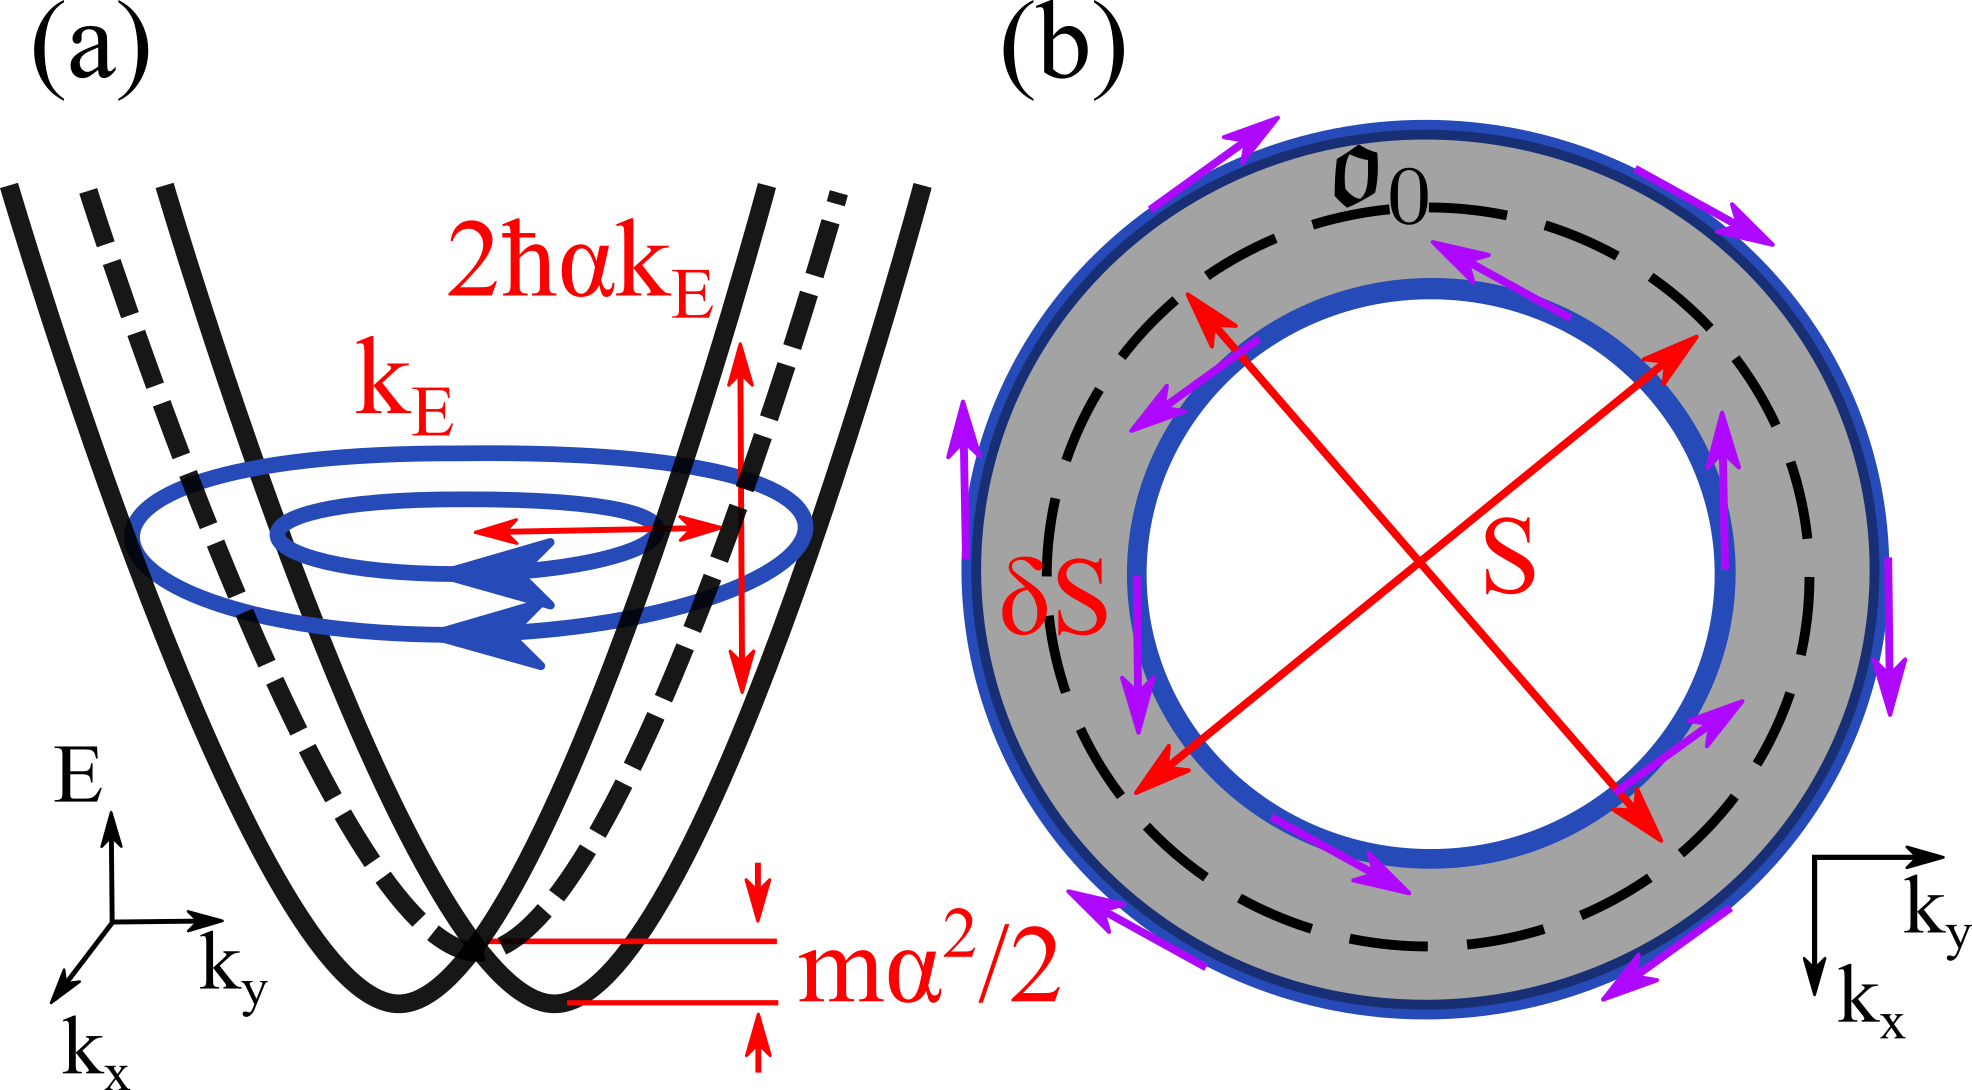
\includegraphics[width=0.9\columnwidth]{orbits.png}
\caption{(a) Solid (resp.\ dashed) lines respectively illustrate the band dispersion of an electron gas with (resp.\ without) Rashba spin-orbit coupling.  The oriented circles illustrate the spin-orit-split orbits for a magnetic field pointing to $-z$ direction. (b) The zeroth-order orbit $\frako_0$ is indicated by a dashed circle with area $S$; $\delta S$ is the differential area  between two spin-orbit-split orbits. The spin texture is indicated by purple arrows.\label{fig:orbits}}
\end{figure}


\subsection{Recovering the Onsager-Lifshitz-Roth quantization rules in two limits}\la{sec:recoveronsager}

It is useful to compare $\delta \var$ with $B\calm$ in the basis of energy-split bands (labelled $\pm$): in the two regimes where one dominates over the other, \qq{eq:rule}{berryconn} reduce to the known Onsager-Lifshitz-Roth rules for (i) two independent, nondegenerate orbits, and for (ii) degenerate orbits.  \\

%\footnote{Though the adiabatic limit does not exist for orbits that exactly intersect at type-II Dirac points, these orbits are nevertheless describable by our quantization rule, as exemplified in the case studies of \s{sec:inplanezeeman} and \s{sec:rotsymmbreakdown}.}}

\noi{i} If $|\var_+{-}\var_-|$ is everywhere (along $\frako_0$) much greater than $B|\calm_{+-}|$, then an electron would undergo adiabatic (band-conserving) dynamics[nenciu] along two independent, nondegenerate orbits. Such an adiabatic regime always exists as $B{\rightarrow} 0$ for quasidegenerate orbits that do not intersect, e.g, at a type-II Dirac point, which is the subject of the case studies in \s{sec:inplanezeeman} and \s{sec:rotsymmbreakdown}.
By  neglecting  $B\calm_{+-}$ in favor of intraband elements,  $\cala$ reduces to a diagonal matrix with  diagonal entries ($e^{i\lambda_{\pm}}$) given by:
\e{\lambda_{\sma{\pm}} = -\int_0^{T_c}\calh_{\sma{\pm\pm}}\f{dt}{\hbar}=\pm \f{1}{2}l^2\delta S - B\int_0^{T_c}\calm_{\sma{\pm\pm}}\f{dt}{\hbar}.  \la{phaseindependentorbit}} 
In the second equality, we have applied \q{spinsplitwkb} and assumed that 
 $\delta \var$ is traceless (this assumption is  valid for splittings of a spin degeneracy\footnote{The Pauli spin-orbit coupling term ${\propto} \bs{\cdot} (\bE {\times} \bp)$ (that is derived from the non-relativistic limit of the Dirac equation) is traceless in any spin-symmetric (pseudo-)spinor basis.  Viewing the spin-orbit coupling as a small parameter in degenerate perturbation theory, the lowest-order splitting of any spin-degenerate energy level is always symmetric about the zeroth-order energy. This follows because the zeroth-order, spin-symmetric wavefunctions (associated to a spin-degenerate level) are tensor products of spin and spatial wavefunctions: $\ket{\Psi_{\pm}}{:}{=}\ket{{\pm}\hat{n}}{\otimes} \ket{\psi}$ with $\hat{n}$ a unit vector and  $\bs{\cdot} \hat{n} \ket{{\pm}\hat{n}}{=}{\pm}\ket{\pm \hat{n}}$. Hence, $\braopket{\Psi_{\pm}}{\bs{\cdot} (\bE {\times} \bp)}{\Psi_{\pm}}{=}{\pm}\hat{n}\cdot\braopket{\psi}{\bE {\times} \bp}{\psi}$. \textbf{Please generalize above proof to the case where H0 already includes centrosymmetric SOC. }}).  \q{eq:rule}, combined with \q{phaseindependentorbit}, may be identified as the Onsager-Lifshitz rule[onsager,lifshitz] for  two independent, nondegenerate orbits of areas $S{\pm}\delta S$, and with subleading phase corrections that were first identified by Roth[rothII].\footnote{We remark that \q{phaseindependentorbit} neglects the contribution by band $-$ to the orbital moment of band $+$: $\delta M_z=il^{-2}\epsilon_{\ab}(\delta \var_+-\delta \var_-)\mathfrak{X}^{\alpha}_{+-}\mathfrak{X}^{\beta}_{-+}$. $\mathfrak{X}^{\alpha}_{+-}$, being an off-diagonal matrix element of the position operator, is generically of order a lattice constant $a$. We then estimate $\int_0^{T_c} B\delta M_z dt/\hbar=O(a^2 \delta S )$, which is negligible compared to $l^2\delta S/2$. Note also that the single-band orbital moment simply vanishes in some symmetry classes of orbits.[100page] } The perturbative inclusion of $B\calm_{\sma{+-}}$ results in  a correction to $\lambda_{\pm}$ [cf.\ \q{phaseindependentorbit}] that is expressible as a power series in $B$, with a leading term proportional to $B$; this will be confirmed in a subsequent case study [cf.\ \q{lambdasmallB}] and applied to understand beatings in quantum-oscillatory phenomena in  \s{sec:qo}.    \\




%the hybridization parameter  $(l^2\delta S)^{-1}$ with the interband matrix elements of the generalized Zeeman interaction $\mathbb{Z}_{+-}{:}{=}B\int_0^{T_c}|\calm_{+-}|dt/\hbar$,  where \qq{eq:rule}{eq:H1} reduce to the known Onsager-Lifshitz-Roth rules for (i) two independent, nondegenerate orbits, and for (ii) degenerate orbits.  \\

%\noi{i} Let us consider the zero-hybridization limit ($l^2\delta S{\gg}1$) for two spin-orbit-split orbits that do not exactly intersect (e.g., at a type-II Dirac point\footnote{Though the adiabatic limit does not exist for orbits that exactly intersect at type-II Dirac points, these orbits are nevertheless describable by our quantization rule, as exemplified in the case studies of \s{sec:inplanezeeman} and \s{sec:rotsymmbreakdown}.}). 

\noi{ii} Let us consider the opposite regime where the Zeeman splitting due to $B\calm$ is much greater than $(\delta \var_+{-}\delta\var_-)$. \qq{eq:rule}{berryconn}, with $\calh{\approx}B\calm$, may then be identified with the quantization rule (formulated previously by us [topoferm,100page]) for degenerate orbits of any symmetry.\footnote{An equivalent but less general formulation was proposed earlier in [RothII] and [Mikitik,Sharlai] for centrosymmetric solids with time-reversal symmetry (at zero field). For comparison, it should be emphasized that \qq{eq:rule}{berryconn} applies to solids of any symmetry, including magnetically-ordered solids.}	   


%The competition between $B\calm$ and $\delta \epsilon$ decides 
%whether the spin-orbit-split energy bands are nontrivially hybridized by the magnetic field. More precisely, the competition is between $\delta \epsilon$ and the inter-band matrix elements of $B\calm$; the former (resp.\ latter) is always dominant for sufficiently weak (resp.\ large) field, as  we will illustrate in the case study of \s{sec:Rashba}. 


%This leading dependence originates from $\A$ being generated by $\delta \var T_c {\propto}1/B$ [cf.\ \qq{eq:prop}{eq:H1}]. 

%One motivation for the form of \q{eq:rule} is a separation of scales for different components of 

%Separating the semiclassical phase (acquired by a spinor wavepacket over one cyclotron period) into multiple components [as in \q{eq:rule}] may be motivated as a separation of scales. 
% in absolute magnitude, the rate of variation of $\partial l^2S$ (with respect to $E$ and $B$) is also much greater.


%Such non-analyticities might originate from saddle- or II-Dirac points of the zero-field Hamiltonian \textit{without} spin-orbit coupling. 





%is estimated to be $\sim\epsilon_c E/\Delta$, much larger than cyclotron energy $\epsilon_c$ due to $\Delta\ll E$. Therefore, the dependence of $\lambda_a$ on $E$ is also weak. 

The quantization rule, summarized by \qq{eq:rule}{berryconn}, is the technical accomplishment of this work; the remainder of this work is focused on unpacking its physical implications. We will first demonstrate the utility of our rule in case studies where the adiabatic approximation is invalid, and $\delta \epsilon$ competes with $B\calm$. There are two conceptually different ways in which the adiabatic approximation may fail: (i) if the spin-split orbits are  symmetric under continuous rotations (as they are for the Rashba 2DEG), then adiabaticity may be lost over the entire orbit [cf.\ \s{sec:Rashba}]. (ii) For asymmetric spin-split orbits, adiabaticity may be lost in the vicinity of a single isolated point, where orbits intersect at a type-II Dirac point [cf.\ \s{sec:inplanezeeman}]. 
In \s{sec:llquasideg}, we investigate how many real parameters are required to tune $\lambda_1{=}\lambda_2$ (mod $2\pi$), which would imply a (near) degeneracy of Landau levels.  

%In the absence of symmetry, three real parameters 
%certain symmetries  reduce the number of tuning parameters to one, as  will be investigated in \s{sec:llquasideg}. 



\section{Case study: Rashba 2DEG with arbitrarily-oriented fields}

%We begin with some preliminary remarks that apply to all case studies in this work. Our chosen studies are modeled (in zero field) by $\bk{\cdot}\bp$ Hamiltonians which are expanded (to quadratic order) about a high-symmetry wavevector ($\bk$). Our model Hamiltonians are written in a (pseudo-)spinor basis, i.e., they are two-dimensional at each $\bk$ [as exemplified by \q{eq:Rashba-Hamiltonian}]; this is the minimal dimension needed to model quasidegenerate orbits. 

%Any (pseudo-)spinor Hamiltonian can be  decomposed, at each $\bk$, into traceful ($\var(\bk)$) and traceless ($\delta \var$) components. We operationally identify the traceful component as the zeroth-order band Hamiltonian (with spin $\text{SU}(2)$ symmetry), and the traceless component as the spin-orbit term; the former produces spin-degenerate energy bands, and the latter splits the degeneracy. This identification has a microscopic justification: the Pauli spin-orbit coupling term  (that is derived from the non-relativistic limit of the Dirac equation) is  traceless in any spin-symmetric  (pseudo-)spinor basis.\footnote{The Pauli spin-orbit term is proportional to  $ \bs{\cdot} (\bE {\times} \bp)$. Viewing the spin-orbit coupling as a small parameter in degenerate perturbation theory, the lowest-order splitting of any spin-degenerate energy level is always symmetric about the zeroth-order energy. This follows because the zeroth-order, spin-symmetric wavefunctions (associated to a spin-degenerate level) are tensor products of spin and spatial wavefunctions: $\ket{\Psi_{\pm}}{:}{=}\ket{{\pm}\hat{n}}{\otimes} \ket{\psi}$ with $\hat{n}$ a unit vector and  $\bs{\cdot} \hat{n} \ket{{\pm}\hat{n}}{=}{\pm}\ket{\pm \hat{n}}$. Hence, $\braopket{\Psi_{\pm}}{\bs{\cdot} (\bE {\times} \bp)}{\Psi_{\pm}}{=}{\pm}\hat{n}\cdot\braopket{\psi}{\bE {\times} \bp}{\psi}$. } $H_0$ determines the zeroth-order orbit $\frako_0$ (and associated action $S$ and cyclotron energy $\var_c$). $H_{so}$ is simply identified with $\delta \var$, the spin-orbit term in the effective Hamiltonian $\calh$. One useful implication of this discussion is that $\delta \var$ is traceless.




\subsection{2DEG with Rashba and Dresselhaus spin-orbit interactions}\label{sec:Rashba}

%[ denoted by $\ket{u_{\pm,\bk}}=(1,\pm e^{i\theta_{\bk}})^t$ with $k e^{i\theta_{\bk}}=k_y+ik_x$ ]

%basis of spin-orbit-split energy  bands (defined at zero field), 

We will first apply our rule to the Landau levels of the Rashba model [cf.\ \q{eq:Rashba-Hamiltonian}], for which analytic expressions exist for verification; shortly after we will demonstrate the utility of our quantization rule for the 2DEG with both Rashba and Dresselhaus spin-orbit interactions, for which there exists no known analytic closed-form solution. 

For simplicity, we assume that the Pauli matrices in \q{eq:Rashba-Hamiltonian} correspond to spin: $s_i{=}\hbar \sigma_i/2$. Let us evaluate the effective Hamiltonian $\calh(\bk)$  along the cyclotron trajectory $\frako_0$ with radius $k$. In the  energy basis of the Rashba Hamiltonian $H_R$ [cf.\ \q{eq:Rashba-Hamiltonian}], 
\e{\calh(\bk)=-\alpha k\tau_z{+}\f{g_s}{2}\mu_{\sma{B}}B\tau_x \red{-} \f{eB\hbar}{2m} (\tau_x-I) \epsilon_{\alpha\beta} k_{\red{\alpha}}\nabla_{\red{\beta}}\theta,\la{rashbaeffham}}
where $\tau_i$ are a new set of Pauli matrices with $\tau_z{=}{+} 1$ and ${-}1$ corresponding to the outer and inner orbits, respectively \red{[I switched the sign in the equation above to emphasize the sign difference.]}. $e^{i\theta_{\bk}}{=}(ik_x{-}k_y)/k$ is the angle of the in-plane spin-orbit field $({-}\alpha k_y,\alpha k_x,0)$, which winds once over $\frako_0$; the spin of our basis vectors likewise winds, in parallel (or anti-parallel) alignment with this field (see Fig. (\ref{fig:orbits})(b)). Terms proportional to the rate of spin rotation  ($\nabk \theta$) originate from the  non-abelian Berry connection. The first term of  $\calh$ corresponds to the spin-orbit-induced splitting of the energy-degenerate bands;
the remaining terms may be interpreted as B-induced deformations of the bands.   It is well-known that the Zeeman term tends to polarize spin in the direction ($\vec{z}$) of $\bB$; remarkably, the non-abelian Berry term   also has a polarizing effect, but with opposite sign. These two effects completely cancel for free electrons ($m{=}m_0$, with $m_0$ being free electron mass.), but not generically in band systems. The orbital moment term $B M_z$, which generally couples the two-band subspace (of interest) to all other bands, is absent in any simplified two-band model.
%Observe that  that $\calh$ is actually time-independent, which originates from a  that is unbroken by the field (aligned with the rotational axis). Consequently, 

Due to the continuous rotational symmetry of $H_R$, $\nabk \theta$ has magnitude $1/k$ and lies tangential to $\frako_0$; consequently, $\calh$ is constant along $\frako_0$, and the propagator simplifies to $\cala{=}e^{{-}i\calh T_c/\hbar}$ without time-ordering, and the phase corrections to the quantization rule are simply the eigenvalues of $\calh$ multiplied by $T_c$:
\begin{equation}
\lambda_{\pm}=\pm\f1{2}\sqrt{({l^2\delta S})^2+\pi^2(g_{\sma{\text{eff}}}-2)^2}+\pi. \label{eq:Rashba-lambda}
\end{equation}
This is a function of the differential action $\delta S$ [cf.\ \q{deltaSvsS}] and  the effective  $g$-factor ($g_{\sma{\text{eff}}}{:}{=}g_sm/m_0$), which is the free-electron $g$-factor multiplied with the ratio of  effective ($m$) and free-electron ($m_0$) masses. The standalone $\pi$ term is the single-band Berry phase associated to the winding of $\theta_{\bk}$ by ${\pm}2\pi$. The two quantities under the square root originate from the spin-orbit energy splitting $\delta \var$ and the inter-band matrix elements of $B\calm$ (in the basis of zero-field bands). 

In the weak-hybridization regime: $l^2\delta S  \gg \pi|g_{\text{eff}}{-}2|$, we may expand \q{eq:Rashba-lambda} as a Laurent series in $B$:
\e{\lambda_{\pm}= \pm \f{l^2\delta S}{2} +\pi \pm \f{\pi^2}{4}\f{(g_{\text{eff}}-2)^2}{l^2\delta S} + O(B^2). \la{lambdasmallB}}
\q{eq:rule}, combined with the first two terms on the right-hand-side of \q{lambdasmallB}, may alternatively be derived from 
the standard Onsager-Lifshitz rules for two independent orbits, with a common $\pi$ Berry-phase correction for each orbit:\footnote{The intra-band Zeeman and orbital-moment couplings vanish due spacetime-inversion symmetry.[topoferm]} $l^2(S{\pm}\delta S)/2\pi {\in}\Z$. Higher-order terms in \q{lambdasmallB} reflect the field-induced hybridization of the spin-orbit-split orbits. 


In the strong-hybridization regime: $l^2\delta S {\ll}\pi(g_{\text{eff}}{-}2)$, $\lambda_{\pm}{\approx}{\pm}\pi g_{\text{eff}} /2$ mod $2\pi$, which corresponds to the Zeeman splitting of Landau levels by $g_{s}\mu_BB$, in the \textit{absence} of the spin-orbit interaction. 

%In the case of free electrons ($m{=}m_0$), we recover  an elementary result in quantum mechanics -- that all levels (except the lowest) are spin-degenerate due to the equality of cyclotron and Zeeman energies. 

%Eq. (\ref{eq:prop}) interpolates smoothly between the quantization rules for degenerate and independent orbits.

%For $\delta\epsilon=0$, Eq. (\ref{eq:prop}) is exactly the propagator for degenerate bands in Ref. [100p].

%If $\delta\epsilon$ dominates over all other terms in \q{eq:H1}, tunneling matrix elements between energy bands may be neglected. That is to say, the propagator is well-approximated by a diagonal matrix in the basis of energy bands; each diagonal element corresponds to the phase offset for an independent orbit.



%To better appreciate this, 
%$\A$ has the form:
%\begin{equation}
%\A=\overline{\exp}[i\oint_\frako_0\left(\begin{array}{cc}
%-\alpha l^{2}mk_F+\frac{1}{2} & -\frac{1}{2}+\frac{g'_s}{4}\\
%-\frac{1}{2}+\frac{g'_s}{4}& \alpha l^{2}mk_F+\frac{1}{2}
%\end{array}\right)d\theta],\label{eq:Rashba-prop}
%\end{equation}
%where $\theta$ is a polar angle parametrizing the cyclotron orbit, and $g_s'{:}{=}g_{s} m/m_0$ is an effective $g$ factor weighted by the ratio of the effective mass $m$ over the free-electron mass $m_0$. Off-diagonal elements of $\A$ induce inter-band tunneling, and are contributed by the Berry connection (the term $-1/2$) and the Zeeman coupling  ($g_s'/4$). That both terms are $k$-independent originate from the continuous rotational symmetry (in $z$ direction) of the Rashba Hamiltonian. 
%Diagonalizing Eq. (\ref{eq:Rashba-prop}), we obtain subleading order correction to quantization rule as

%The two quantities under the square root reflect a competition between intra- and inter-band matrix elements. The latter reflects a quantum interference between the Zeeman coupling and the non-abelian Berry connection, which is captured by our quasidegenerate quantization rule but absent in the standard Onsager-Lifshitz rules for independent orbits. To appreciate this, suppose we employ the standard rules[roth,100page] and properly account for the Zeeman coupling, the orbital moment, and the single-band Berry phase. The  Zeeman coupling  modifies the zero-field energy bands in two ways: it enlarges the spin-orbit-induced energy gap as $\Delta {\rightarrow} \Delta'{:}{=} \sqrt{(\Delta)^2{+}(g_s\mu_BB)^2}$, and it tilts the spin (along either orbit) out of the xy-plane. For $\Delta'{\gg}\var_c$, we may treat each Zeeman-deformed orbit as independent, and the corresponding Onsager-Lifshitz quantization rules are 
%\e{ l^2S\pm \lambda'_{\pm} = 2n(\pi+1/2), \;\text{with}\;   \lambda'_{\pm}:=\pm 2\pi \Delta'/\var_c{+}\pi.}
%The first component of $\lambda'$ is simply the modification of the WKB phase $l^2\delta S'$ due to both spin-orbit and Zeeman couplings; the second component is  the sum (${=}\pi$)[Fuchs,topoferm] encodes the single-band Berry phase and the orbital moment. A comparison of $\lambda_{\pm}$ with $\lambda'_{\pm}$ shows that the former has an extra $1/2$ under the square root [cf.\ \q{eq:Rashba-lambda}], which originates from the off-diagonal element of the non-abelian Berry connection. In other words, the standard Onsager-Lifshitz rules neglects the aforementioned quantum interference. This interference is completely destructive for free electrons ($m{=}m_0$), but not generically in band systems.

%\footnote{We have further assumed here that basis functions of $\mathcal{H}_R$ are eigenstates of spin operator $s_z$, which also need not be true in band systems. }

Our quantization rule [\q{eq:rule} with \q{eq:Rashba-lambda}] may be compared with the  exact Landau-level spectrum of the Peierls-substituted Hamiltonian $H_R(\bK)$. The exact levels are given implicitly by
\e{
&n_{\pm}=\frac{l^2S}{2\pi}+\frac{l^2\delta S}{16\pi}\f{\delta S}{S}\lin 
&\pm\f1{2}\sqrt{\bigg(\frac{l^2\delta S}{8\pi}\f{\delta S}{S}\bigg)^2+(l^2\delta S)^2+\pi^2(g_{\sma{\text{eff}}}-2)^2},\label{eq:Rashba-exact}}
with the functional forms of $\delta S(E)$ and $S(E)$ provided in \q{deltaSvsS};  $n_{+}{\ge} 1$ and $n_-{\ge} 0$ here are integer-valued labels for two distinct sets of levels.  In the quasidegenerate regime ($E{\gg}m\alpha^2$), terms involving $\delta S/S$ may be neglected and \q{eq:Rashba-exact} reduces to our quantization rule with $\lambda_{\pm}$ given by \q{eq:Rashba-lambda}.

Our quantization rule equally has utility where no closed-form analytic expression exists for the spectrum. Such is the case when we introduce a Dresselhaus spin-orbit coupling:
\begin{equation}
 H_{RD}(\bk)=\frac{{\hbar^2}k^2}{2m}+\alpha(k_{x}\sigma_{y}-k_{y}\sigma_{x})+\beta(k_{x}\sigma_{x}-k_{y}\sigma_{y}).\la{hamRD}
\end{equation}
In Fig. \ref{fig:RD}(b), a comparison is made between the Landau levels obtained from exact numerical diagonalization of $H_{RD}(\bK)$ (by standard techniques reviewed in App. \ref{sec:numerical}) and those obtained from the quantization rule. The difference in energies  does not exceed $2\%$ of $\var_c$ [cf.\ \fig{fig:RD}(c)] for various choices of the spin-orbit parameters $(\alpha,\beta)$.
Larger differences are positively correlated with 
$l^2\delta S^2/S$ (with $\delta S$ depending on both $\alpha$ and $\beta$), as shown in Fig. \ref{fig:RD}(d); see also \q{eq:Rashba-exact}, which analytically demonstrates how terms involving $l^2\delta S^2/S$ modifies the quantization rule in the case $\beta=0$. 

In \s{sec:llquasideg} we will further motivate the study of $H_{RD}$ by investigating the prevalence of Landau-level degeneracies. 


%\red{Equation \ref{eq:Rashba-exact} indicates the error of quantization rule is mainly contributed by high order terms, such as terms proportional to $l^2 \delta S^2/S$. We plot in Fig. \ref{fig:RD}(c) $l^2 \delta S^2/S$, showing a strong positive correlation between $l^2 \delta S^2/S$ and error of quantization rules. 

%For a last numerical comparison, we plotted in Fig. \ref{fig:RD} (b) the Landau-level spectrum at fixed $\alpha$ and $\beta$ 

%For fixed $\alpha$ and $\beta$, Landau fan diagrams are presented in Fig. \ref{fig:RD} (b), showing perfect match at relatively large magnetic field and slight deviation in smaller magnetic field between quantization rule and exact Landau levels. 

%A typical constant energy contour of the band structure is shown in Fig. \ref{fig:errors} (a), where Dresselhaus SOC breaks continous rotational symmetry to two fold rotational symmetry. There are no known analytic closed-form solutions to the magnetic Hamiltonian $H_{RD}(\bK)$ obtained by Peierls subtitution of $H_{RD}(\bk)$; however $H_{RD}(\bK)$ can be numerically diagonalized by standard techniques that are reviewed in App. \ref{sec:numerical}. The difference between $\lambda$ calculated by numerical diagonalization and by Eq. \ref{eq:prop} are shown in Fig. \ref{fig:errors} (c), where good agreement can be observed. $\Delta/\epsilon_c$ of corresponding parameter range is presented in Fig. \ref{fig:errors}(b).

%$\lambda$ extracted from from Eq. (\ref{eq:Rashba-exact}) is consistent with what we have obtained in Eq. (\ref{eq:Rashba-lambda}). 

%It is instructive to consider what we would have obtained if we ignore the tunneling between the quasidegenerate orbits. Without tunneling, the quantization rule gives Eq. (\ref{eq:Rashba-exact}) with $(1/2-g_s'/4)^2$ missing under the square root. This difference is only relevant when $\epsilon_s$ is small enough such that this term dominates the square root, i.e., in the quasidegenerate range.

\begin{figure}
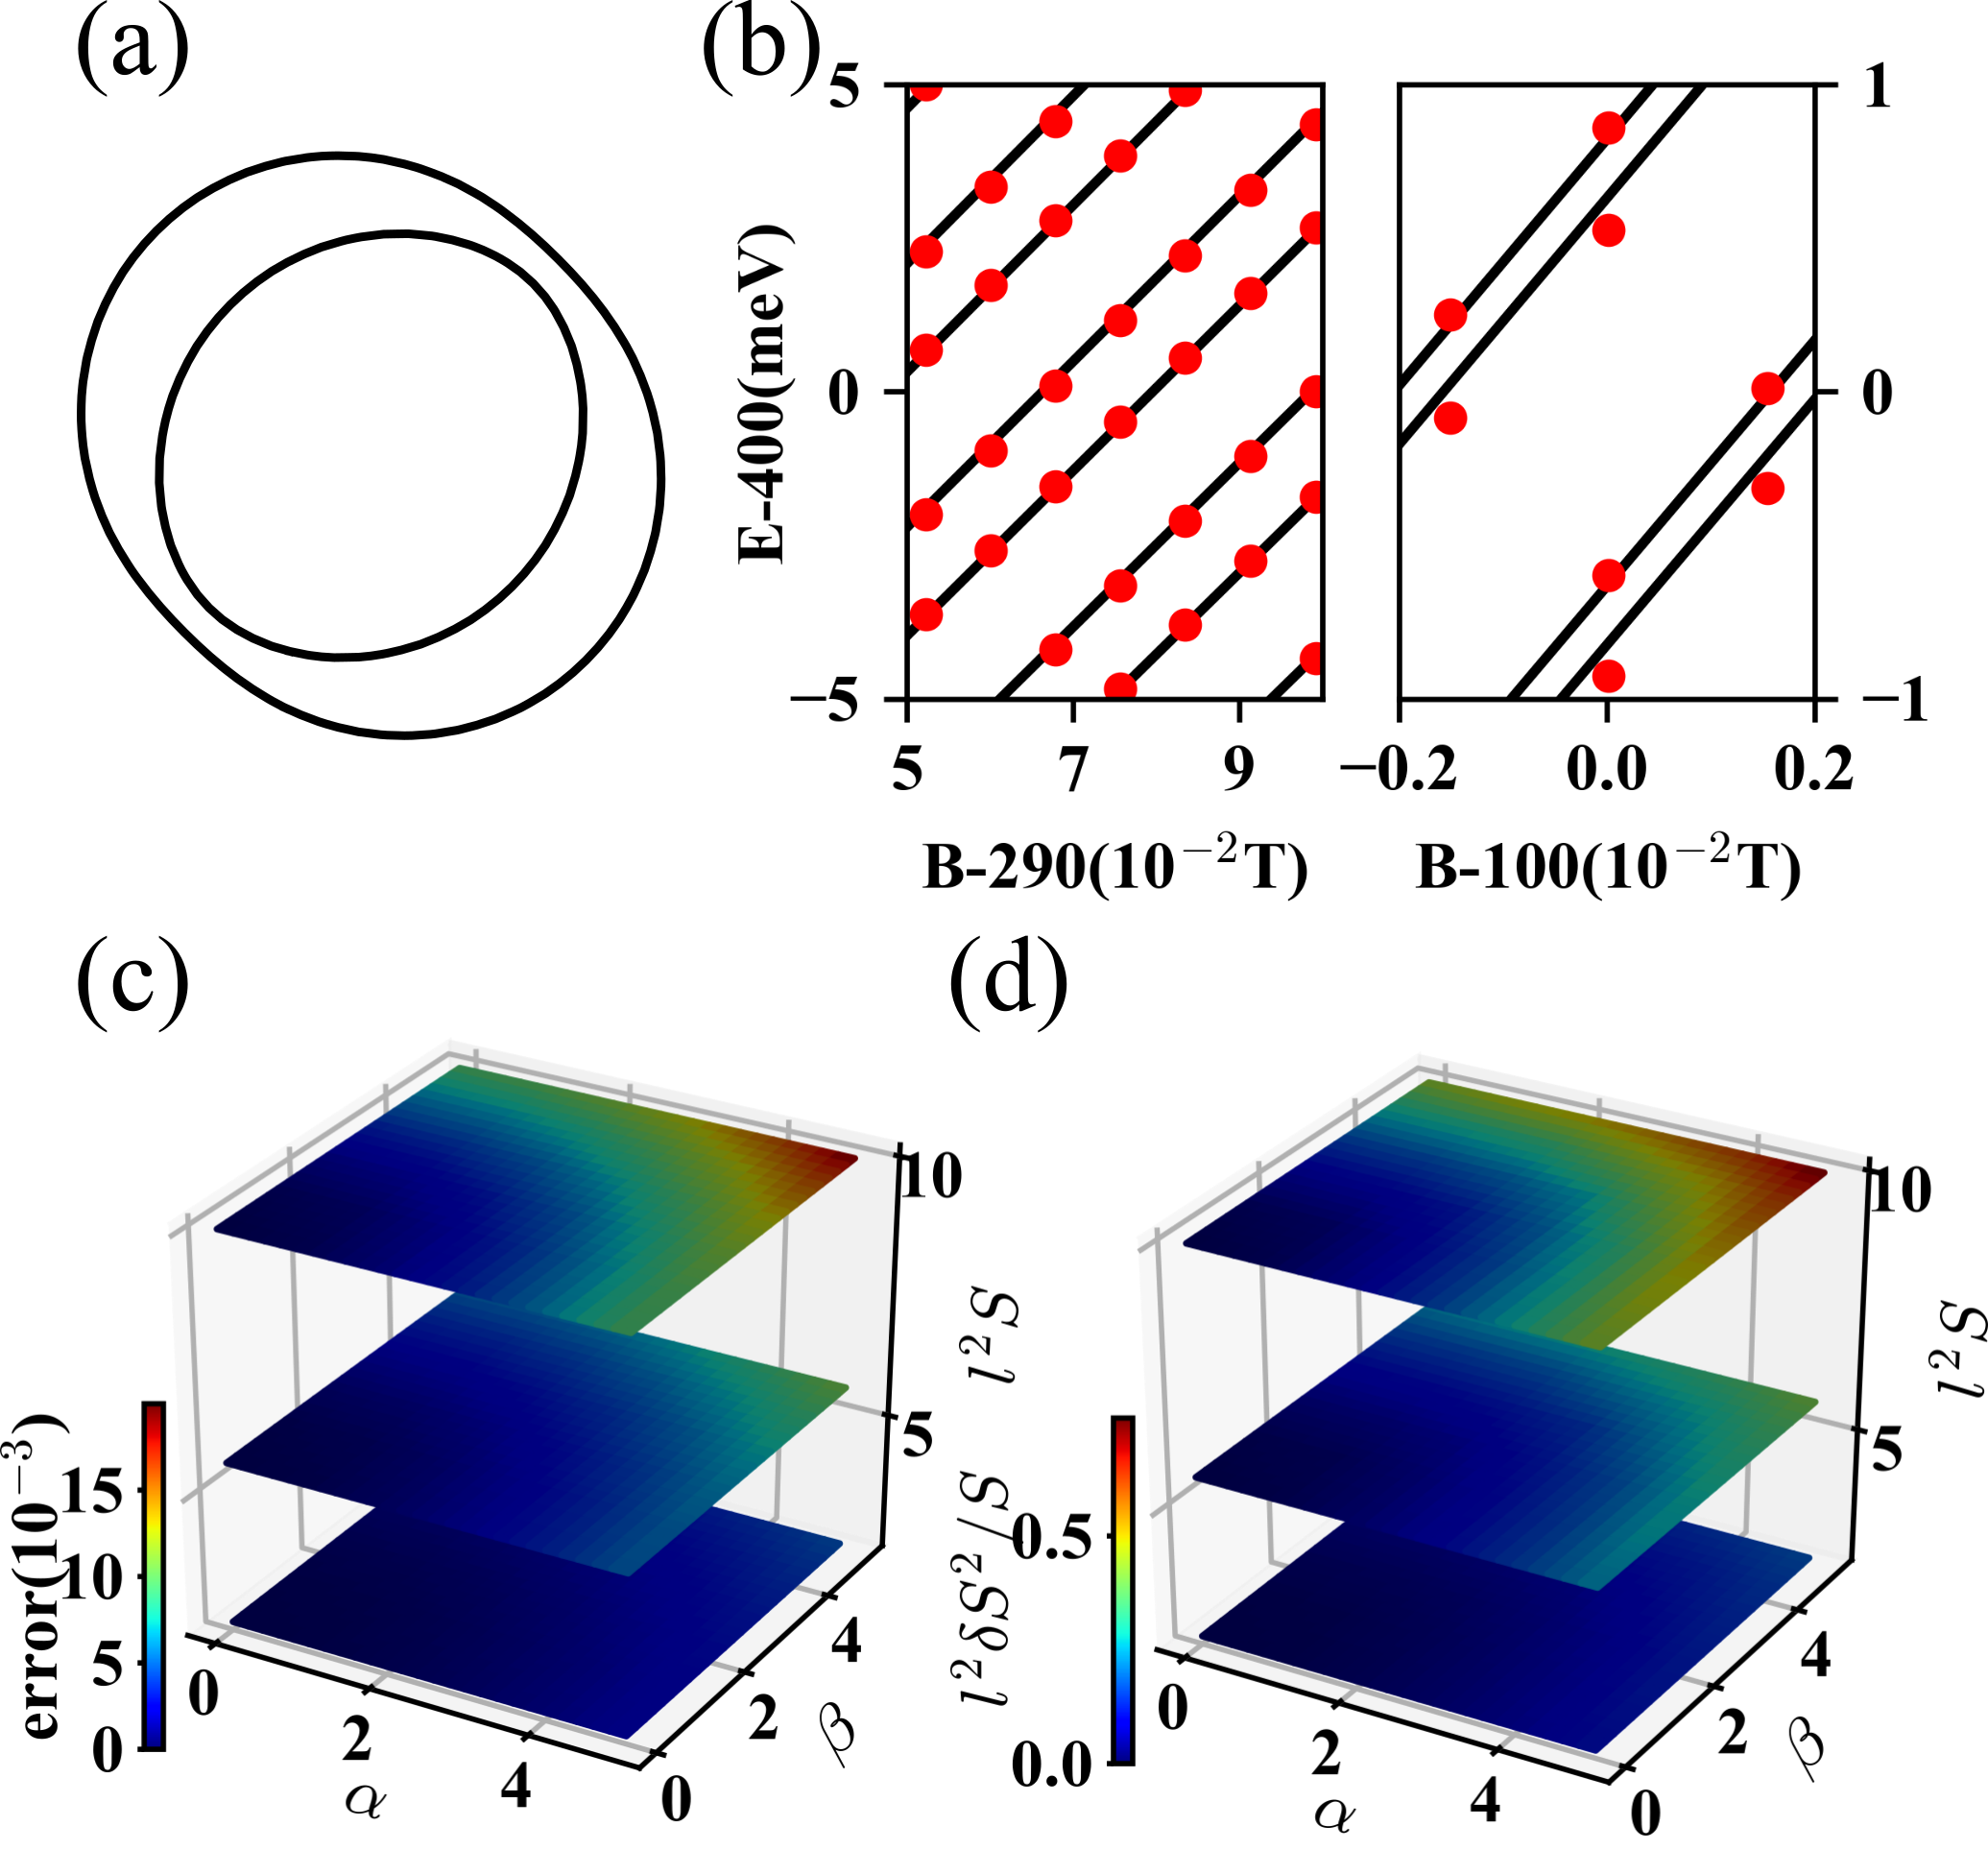
\includegraphics[width=1.0\columnwidth]{RD.png}
% alpha=0.05
% beta=0.02
% m=0.01
\caption{Rashba-Dresselhaus model. (a) Typical cyclotron orbits. (b) Comparison of Landau levels calculated by Eq. (\ref{eq:rule}) (black lines) and numerical diagonalization of the Peierls-Onsager Hamiltonian  $H_{RD}(\bK)$ (red dots). Parameters for (b): $\alpha=0.05$(eV$\cdot$\AA), $m=0.01$($\hbar^2$/eV$\cdot$\AA$^2$), $\beta=0.02~(0.04)$(eV$\cdot$\AA) for left (right) panels. $B$ is measured from 2.9 and 1.0T respectively and is in unit $10^{-2}$T. (c) For various spin-orbit parameters $(\alpha,\beta)$ of the Rashba-Dresselhaus model and various field strength (satisfying $l^2S(E)\gg 1$), we plot  $\text{error}:=|\epsilon_\text{rule}-\epsilon_\text{exact}|/\var_c$ for a single Landau level that lies closest to energy $E=0.4eV$, where $\epsilon_\text{rule}$ is determined by Eq. (\ref{eq:rule}) and $\epsilon_{\text{exact}}$ is obtained by numerical diagonalization of the Peierls-Onsager Hamiltonian  $H_{RD}(\bK)$. We also plot in (d) $l^2\delta S^2/S$, which has a strong positive relation with error in (c). Parameters for (c-d): $m=0.01$($\hbar^2$/eV$\cdot$\AA$^2$). Units: $\alpha$($10^{-2}$eV$\cdot$\AA), $\beta$($10^{-2}$eV$\cdot$\AA), $Z$($10^{-3}$eV), $l^2 S$($10^2$).\label{fig:RD}}
\end{figure}

\subsection{Rashba 2DEG with in-plane Zeeman field}\la{sec:inplanezeeman}


Our next case study involves orbits that (nearly) touch at a type-II Dirac point -- an asymmetric variant of the conventional Dirac point (as will be introduced below). Quantum tunneling localized to a type-II Dirac point  (in short, II-Dirac point) is known to be mathematically equivalent to  Landau-Zener breakdown, with the electric force replaced by the Lorentz force. [Blount, Obrien, AALG] First, we will demonstrate how we recover Landau-Zener dynamics in the weak-hybridization regime  of \qq{eq:rule}{eq:H1}. 

%With intermediate hybridization , including the regime where Landau-Zener dynamics is non-applicable and breakdown is nonlocal.  

We begin again with the Rashba model of a rotationally-symmetric Dirac cone. To convert this Dirac point to its asymmetric variant, 
let us introduce a Zeeman coupling to an in-plane magnetic field $B_\parallel$ (parallel to the $+y$ direction):
\e{ 
H_{RZ}=\f{{\hbar^2}k^{2}}{2m}+\alpha(k_{x}\sigma_{y}-k_{y}\sigma_{x})+\zpar\sigma_{y}, \la{eq:RZ-Hamiltonian}}
with $\zpar{:}{=}{g_s}\mu_B B_{\parallel}/2$.
While this field breaks both time-reversal ($T$) and two-fold rotational ($C_2$) symmetries, the composition $C_2T$ is preserved as $\sigma_x H^*_{RZ}(\bk)\sigma_x{=}H_{RZ}(\bk),$ which constrains spin to lie in-plane at each $\bk$. In this symmetry class, Dirac nodes are irremovable but movable   in two-dimensional $\bk$-space. The in-plane Zeeman field has the dual effect of  moving the Dirac node  to the position:
\begin{eqnarray}
\bar{k}_x & = & -\frac{\zpar}{\alpha},\;\bar{k}_y=0,\;\epsilon_{0}=\frac{{\hbar^2}\zpar^{2}}{2m\alpha^2},\label{whereisdiracpoint}
\end{eqnarray}
and tilting the Dirac cone. To observe this tilt, consider the linearized Hamiltonian in the vicinity of this node: 
\e{
H & =\alpha\left[\left(\sigma_y-\frac{{\hbar^2}\zpar}{m\alpha^2}\right)\delta k_{x}-\delta k_{y}\sigma_{x}\right]+\epsilon_{0}.}
When $|\hbar^2\zpar|>|m\alpha^2|$, the Dirac cone tilts over in the $x$ direction, leading to a Lifshitz transition  of the constant-energy band contours -- from circular to hyperbolic (in the linearized approximation), as illustrated in Fig. \ref{fig:RZ}(c). An over-tilted Dirac cone shall be referred to as type-II. Our case study of a II-Dirac point  connects  two electron-like  pockets [cf.\ \fig{fig:RZ}(a,c)], and  differs from previous case studies [Obrien, AALG] that connect an electron- and hole-like pocket.

\begin{figure}
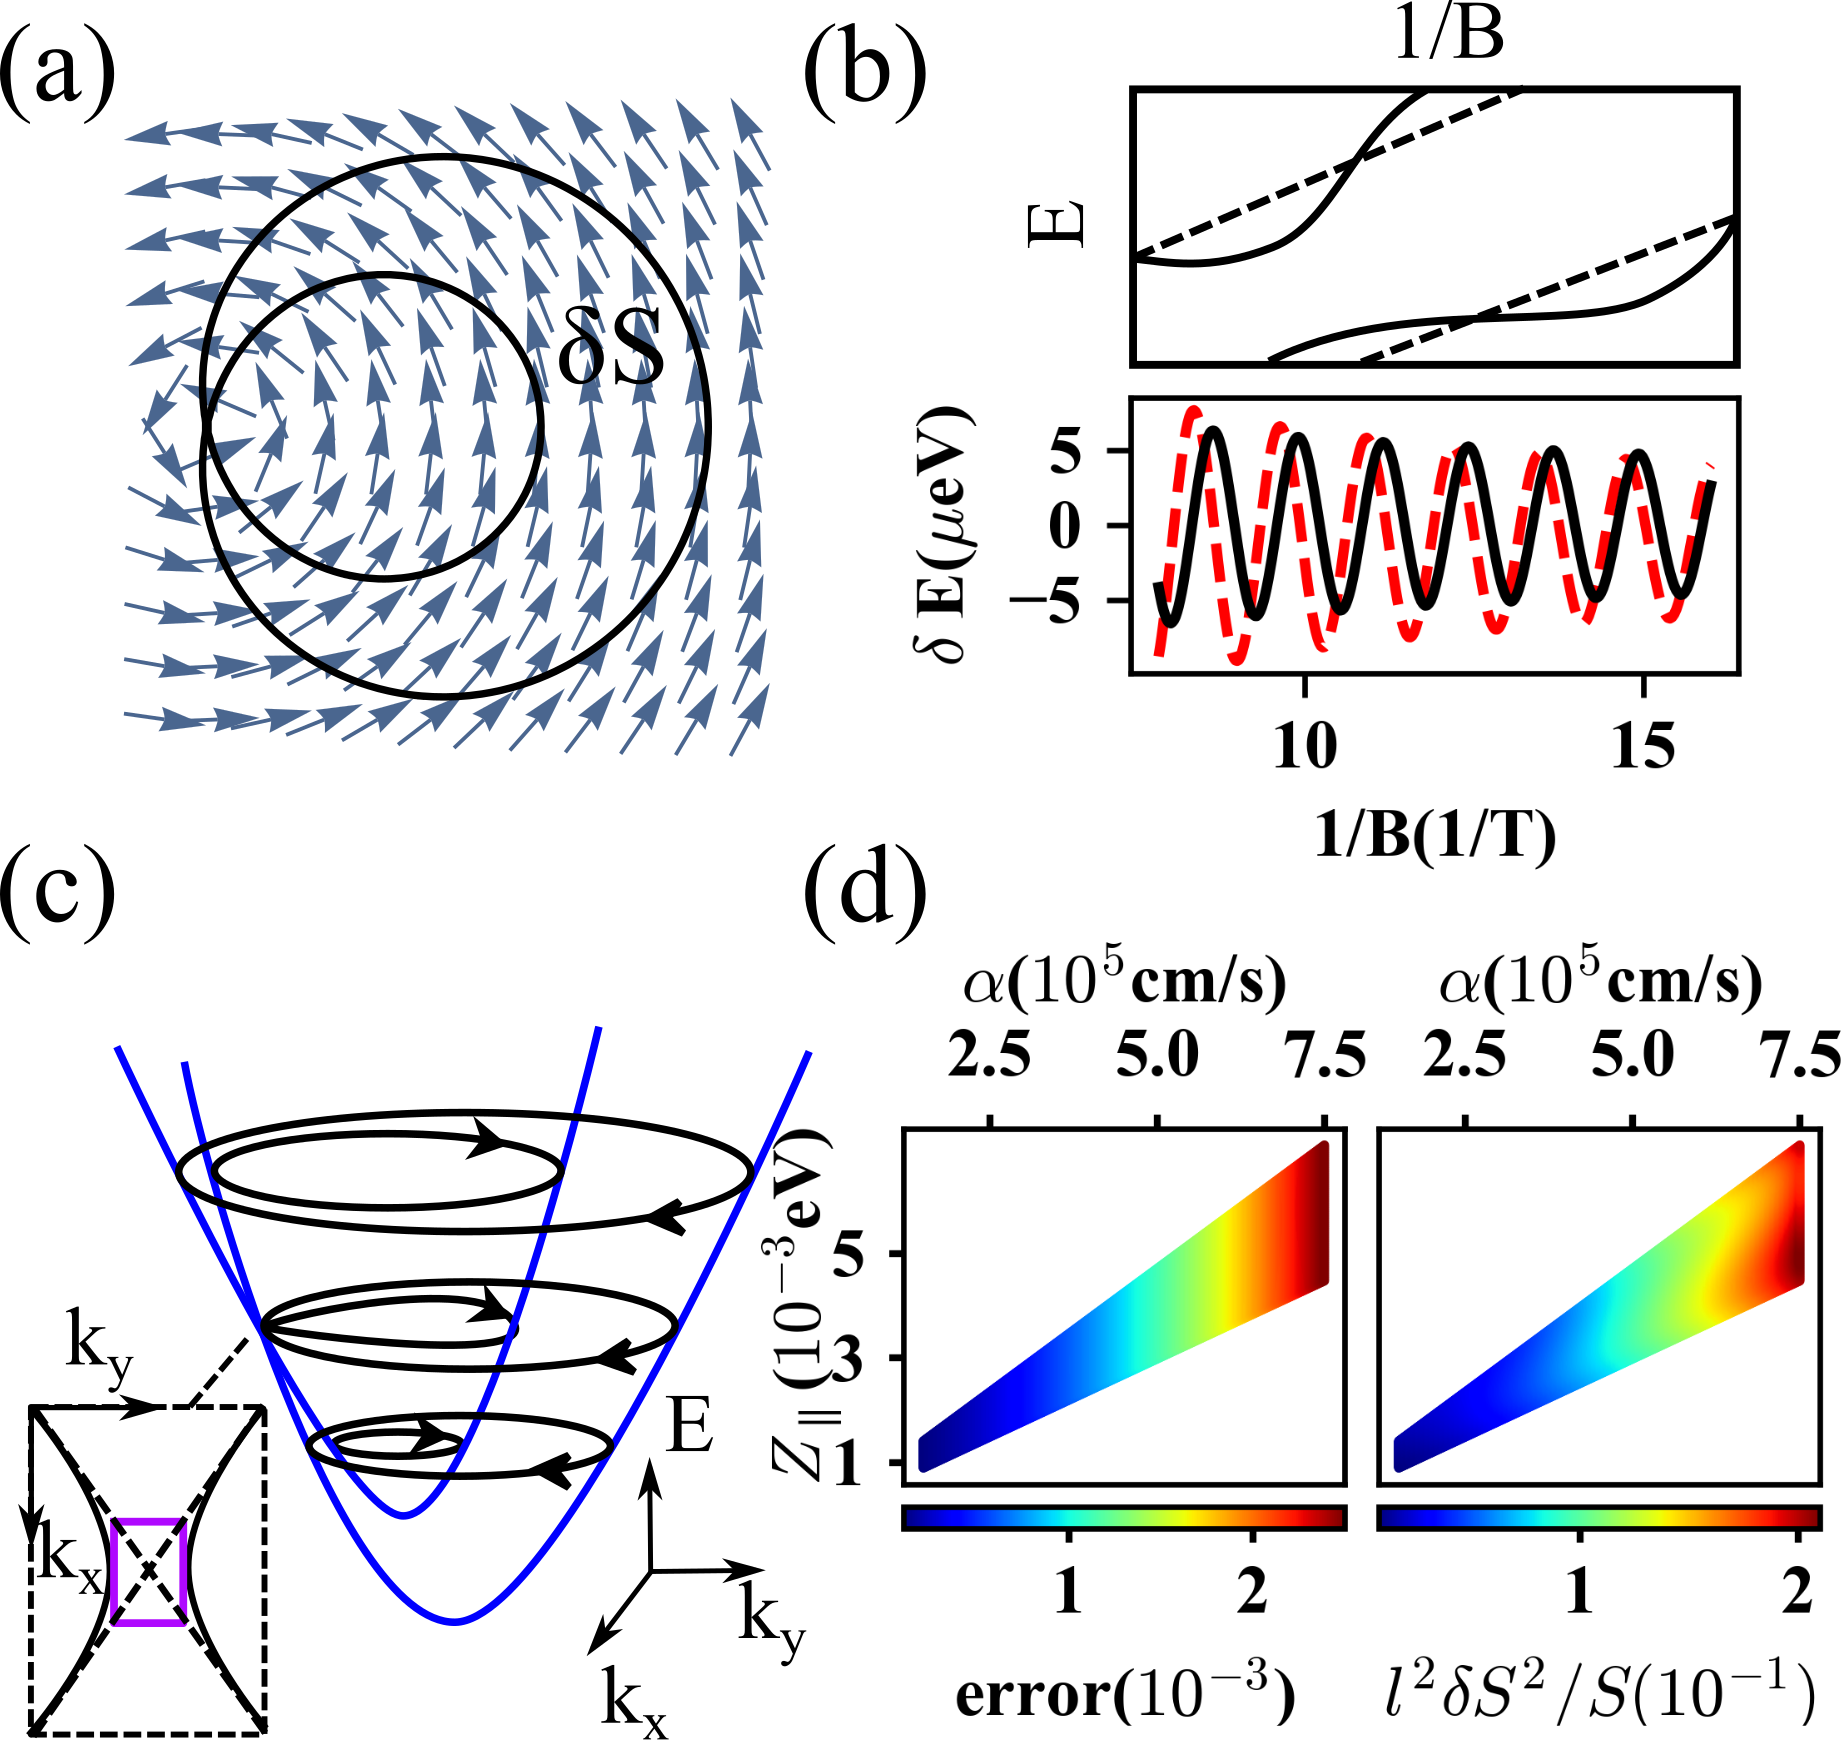
\includegraphics[width=1.0\columnwidth]{RZ.png}
\caption{(a) Trefoille-shaped cyclotron orbit for the Rashba-Zeeman model at the energy of the Dirac point. The orbit is drawn over the  {spin-orbit field} ($d_x,d_y$) of the Hamiltonian $H_{RZ}{=}d_0(\bk)I{+}d_x(\bk)\sigma_x{+}d_y(\bk)\sigma_y$, with $d_j$ obtainable from \q{eq:RZ-Hamiltonian}. The wavefunction along the inner (resp.\ outer) component of the trefoille orbit has its pseudospin aligned parallel (resp.\ anti-parallel) to the spin-orbit field. (b) Black dashed lines illustrate a zeroth-order approximation of the Landau levels (assuming Klein tunneling); the leading-order correction is indicated by red lines. The Dirac point lies at $10$meV. Parameters for (b): $m$: 0.02$\hbar^2$/eV$\cdot$\AA$^2$, $\alpha$: 0.05eV$\cdot$\AA, $Z_\parallel$: 0.001eV. (c)\textbf{ Can we add axes E vs kx vs ky for main figure, and another set of axes kx vs ky for inset?} A sketch of cyclotron orbits of Rashba Hamiltonian with in-plane magnetic field. (d) For various configurations ($\alpha$, $Z_\parallel$) of $H_{RZ}$, we plot in left panel $\text{error}:=|\epsilon_\text{rule}-\epsilon_\text{exact}|/\var_c$ for a single Landau level that is closest to $\epsilon_0$ in Eq. (\ref{whereisdiracpoint}), where $\epsilon_\text{rule}$ is determined by Eq. (\ref{eq:rule}) and $\epsilon_{\text{exact}}$ is obtained by numerical diagonalization of the Peierls-Onsager Hamiltonian $H_{RZ}(\bK)$. Corresponding $l^2 \delta S^2/S$ are plotted in right panel. We only plotted in region where $0.4<\epsilon_0<1.0$(eV).\footnote{$l^2S\gg 1$ is assured by requiring $\epsilon_0>0.4$; the reason of choosing $\epsilon_0<1.0$ is Dirac point lying at high energy requires too much harmonics in numerical diagonalization. This requirement is equivalent to $\sqrt{0.8m}\alpha/\hbar<Z<\sqrt{2m}\alpha/\hbar$, corresponding to the boundaries of the plots in (d).} Parameters for (d): $m$: 0.01$\hbar^2$/eV$\cdot$\AA$^2$, $l=100$\AA. \textbf{please choose formatting such that footnote is at the back} \label{fig:RZ}}
\end{figure}

In addition to the in-plane field, let us also apply an out-of-plane field $B_{\perp}$, with associated magnetic length $\lper{=}\sqrt{\hbar/eB_{\perp}}$, cyclotron energy $\var^{\sma{\perp}}_c{:}{=}\hbar^2/m\lper^2{:}{=}\hbar \omega_c^{\sma{\perp}}{:}{=}h/T_c^{\sma{\perp}}$ and Zeeman coupling to the spin magnetic moment:  $\zper{:}{=}{g_s}\mu_B B_{\perp}/2$. It is assumed that $\lper^2S$ is large, where $S$ is the area of the zeroth-order orbit (with effective mass $m$). For energies much greater than $m\alpha^2$ and $\zpar$, the quasidegeneracy condition is met: $\delta S{\ll}S$, hence we may apply the quantization rule of \qq{eq:rule}{eq:H1} in the subsequent analysis. 

As alluded to in \s{sec:qtznrules}, the adiabatic limit of two independent orbits does not exist if the two spin-orbit-split orbits exactly intersect at a II-Dirac point. To investigate this failure of adiabaticity, let us study the Landau levels at energies close to the II-Dirac point ($\epsilon_0$). We focus first on the regime where, on average (over $\frako_0$), the energy splitting $|\delta \var_+{-}\delta \var_-|$ (due to both  spin-orbit and in-plane Zeeman interactions) is much greater than the interband, out-of-plane Zeeman interaction $B_{\perp}|\calm_{\pm}|$. This implies that the split orbits do not appreciably hybridize -- except in the vicinity of the II-Dirac point where orbits (nearly) touch. Near this II-Dirac point, the dynamics of a two-component wavepacket is described 
 by the effective Hamiltonian
\e{
\calh = \alpha k_{E} \,\omega^{\sma{\perp}}_c t\,\sigma_x+(Z_\parallel-\alpha k_{E})\sigma_y-Z_\perp\sigma_z,\la{effhamIIDirac}
}
with $k_E{=}\sqrt{2mE}/\hbar$ and  $t$ a time variable which parametrizes the zeroth-order orbit:
$\bk(t){=}({-}k_E \cos \omega_c^{\sma{\perp}} t, k_E \sin \omega_c^{\sma{\perp}} t ).$ 
$\calh$ above has been linearized with respect to  $t$, which vanishes in the vicinity of the Dirac point. The eigenbasis of $\sigma_x$ corresponds to two diabatic levels with characteristic slope $v_d{:}{=}\alpha k_E\omega^{\sma{\perp}}_c$; near $t{=}0$, the diabatic levels anticross  due to the hybridization terms proportional to $\sigma_{y,z}$. Generally, the probability of tunneling across the hybridization-induced barrier is  $\rho^2{=}\exp(-2\pi\barmu)$, with $\barmu{=}{E_g}^2/{2v_d \hbar}$ and $E_g$ the energy gap at the center of the anticrossing;[Landau and lifshitz, Wittig] in this context,
\e{\barmu=\frac{Z_\perp^2+(Z_\parallel-\alpha k_{E})^2}{2\alpha k_{E}\var^{\sma{\perp}}_c}, \la{mu1}}
with $2\alpha k_E$ the spin-orbit splitting at energy $E$ [cf.\ \fig{fig:orbits}(a)]. In the absence of the out-of-plane Zeeman coupling ($Z_\perp{=}0$), $\bar{\mu}$ would vanish at the energy of the II-Dirac point -- leading to unit-probability Klein tunneling, as was first proposed by [Obrien] in a different model realization of the II-Dirac point. However, with a proper account of $Z_\perp$, we find instead that $\bar{\mu}$ has a nonvanishing minimum: $\bar{\mu}_{\sma{\text{min}}}{:}{=} (m/m_0)(Z_\perp/2\alpha k_{E})$, which is a product of the dimensionless effective mass and the ratio of the out-of-plane Zeeman splitting over the spin-orbit splitting. This minimum is practically negligible for  semiconductor heterostructures with $m{\ll}m_0$, but may be relevant in heavy-fermion systems. 


To determine the Landau levels, one needs not just the probability for tunneling but also the phase of the probability amplitude. The full information is encoded in a scattering matrix [AALG]
\e{\mathbb{S}=\matrixtwo{\tau e^{i\barphi}}{-\rho}{\rho}{\tau e^{-i\barphi}},\;\rho=e^{-\pi\barmu},\;\tau=\sqrt{1-\rho^{2}}\la{scattmat}}
which is a connection formula that matches the two-component semiclassical (WKB) wavefunction across the Dirac point. $\mathbb{S}$ in \q{scattmat} has been expressed in the basis of spin-split energy bands, so  the diagonal elements of $\mathbb{S}$ are amplitudes for intraband (adiabatic) transmission; the phase of this amplitude is $\barphi{:}{=}\barmu{-}\barmu\ln\barmu{+}\text{arg}[\Gamma(i\barmu)]{+}\pi/4$ with $\Gamma$ the gamma function. 

Away from the II-Dirac point, a semiclassical wavepacket undergoes adiabatic (band-conserving) dynamics. The time-ordered, coherent process of interband tunneling and adiabatic dynamics is described by the propagator:
\e{{\A}= \matrixtwo{\tau e^{i\bar{\varphi}}}{-\rho}{\rho}{\tau e^{-i\bar{\varphi}}} \diagmatrix{e^{i\tilde{\lambda}_+}}{e^{i\tilde{\lambda}_-}}. \la{propinplanezeeman}}
$\tilde{\lambda}_{\pm}$ is generated by $\H_{\pm \pm}$ and has the same form as \q{phaseindependentorbit}, with $B\int_0^{T_c}\calm_{\pm\pm}dt/\hbar$ equal (in this model) to the single-band Berry phase ($\phi_{\pm}^B$) of band $\pm$ on $\frako_0$. At energies far above the Dirac point ($|E{-}\epsilon_0|{\gg}|Z_{\perp}|$) where the Zeeman interaction is negligible, both orbits encircle the Dirac point and hence $\phi_{\pm}^B{\approx}{\pm}\pi$; far below the Dirac point, neither orbit encircles the Dirac point, leading to $\phi_{\pm}^B{\approx}0$. At intermediate energies, $\phi_{+}^B$ (resp.\ $\phi_{-}^B$) is a continuous and increasing (resp.\ decreasing) function of energy, as supported by the Bloch-sphere argument in Fig. \ref{fig:blochsphere}.


%{=}\int_{\sma{0}}^{\sma{T_c}}\calh_{jj}dt/\hbar$ is the cyclotron integral of the corresponding diagonal element of the effective Hamiltonian (in the energy-band basis). $\delta \Omega_{\pm}{=}{\pm}l^2\delta S/2$ plus a field-independent geometric phase (equal to the angle swept by the in-plane spin-orbit field $(\bk^2/2m_2{-}\mu,wk_x,0)$ along the spin-split trajectory; cf.\ discussion in \s{sec:Rashba}).  

\begin{figure}
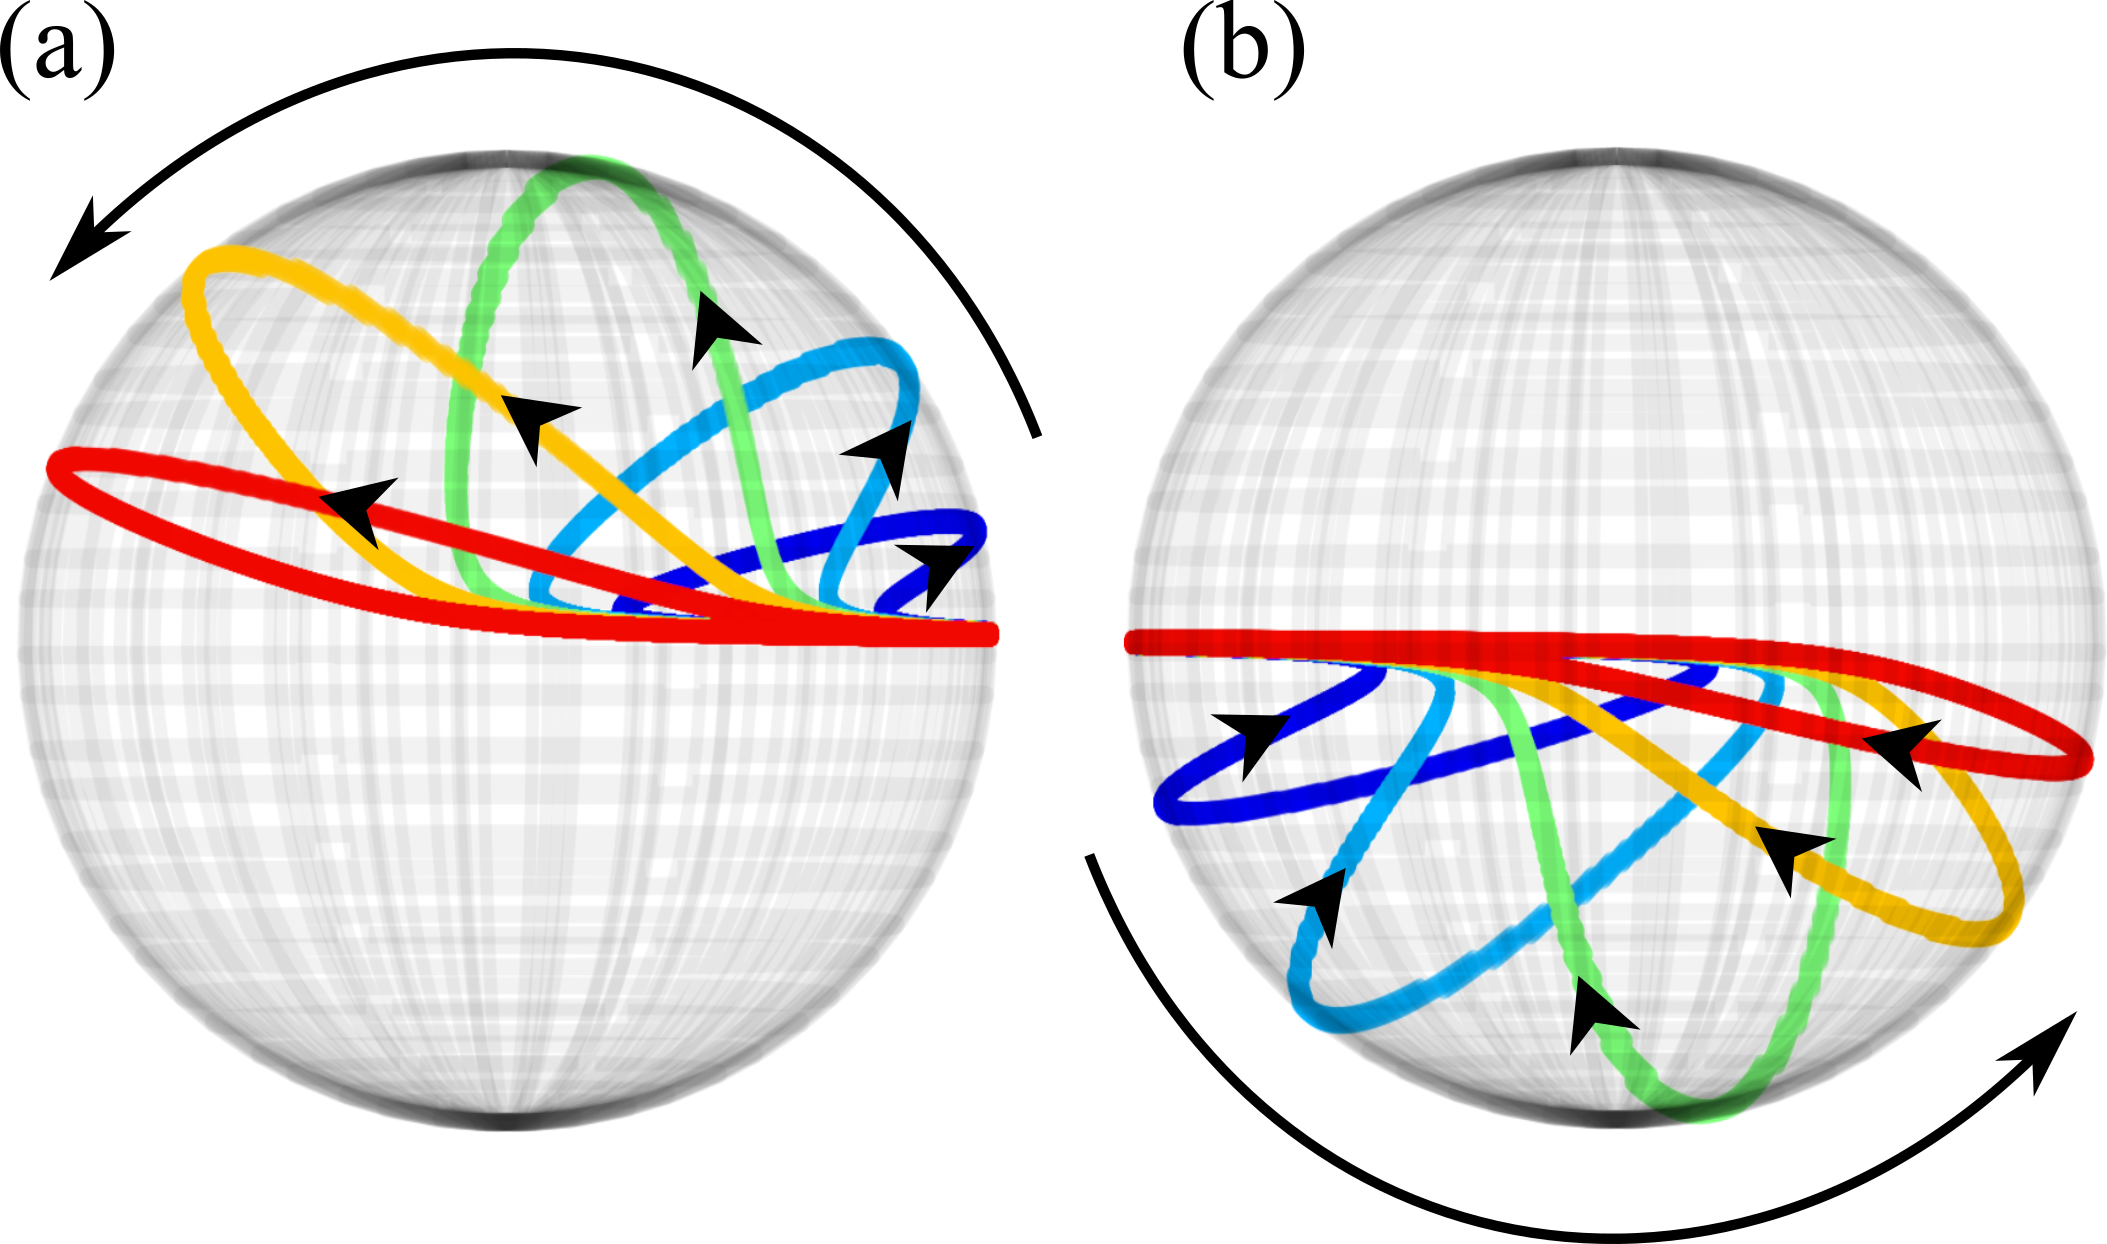
\includegraphics[width=0.8\columnwidth]{blochsphere.png}
\caption{Energy dependence of the Berry phase for inner [(a)] and outer [(b)] orbit. The Berry phase equals half the solid angle enclosed by the corresponding loop on the Bloch sphere \textbf{[loop must be explained, right-hand rule explained]}. The directions of the loops are indicated by black arrows and the black arrow outside of the sphere indicates increasing energy, where green lines correspond to $\epsilon_0$ in Eq. (\ref{whereisdiracpoint}) \textbf{This figure is problematic because only the red loop is shown, while for the other loops the audience is left guessing. Perhaps it is best to separate one bloch sphere into three smaller spheres, such that each smaller sphere has only one loop. We might also show the analog of Fig 3a for energy above and below Dirac point.}.\label{fig:blochsphere}}
\end{figure}

Our quantization rule [\qq{eq:rule}{eq:H1}], with $\A$ having the form of \q{propinplanezeeman}, may be equivalently expressed as
\e{
\text{cos}\left[\frac{\Omega_{-}+\Omega_{+}}{2}\right]=\tau\,\text{cos}\left[\frac{\Omega_{-}-\Omega_{+}}{2}+\bar{\varphi}\right], \lin
\ins{with}\;\Omega_{\pm}=l^2 (S\pm \delta S/2)+\phi_{\pm}^B +\gamma_{\pm}, \la{coscos}
}
$\Omega_{\pm}$ is the phase acquired by an electron in adiabatically traversing orbit $\pm$; the quantum Maslov correction $\gamma_{\pm}{=}\pi$ for circular orbits. A quantization rule analogous to \q{coscos} was previously derived by us for a II-Dirac point that intermediates an electron- and hole-like orbit [AALG]. 

%Let us first investigate the minimal- and maximal-tunneling limits for \q{coscos}. At energies away from the Dirac point ($E{\neq}\epsilon_0$) and in the limit $B{\rightarrow}0$, Landau-Zener tunneling is negligible ($\tau{\rightarrow}1,\bar{\varphi}{\rightarrow}0$), and \q{coscos} simplifies to the Onsager-Lifshitz-Roth rules ($\Omega_{\pm}/2\pi{\in}\Z$) for  two independent orbits. 

In the limit $B{\rightarrow}0$ (equivalently, $\bar{\mu}{\rightarrow} \infty$), Landau-Zener tunneling is negligible ($\tau{\rightarrow}1,\bar{\varphi}{\rightarrow}0$), and \q{coscos} simplifies to the Onsager-Lifshitz-Roth rules ($\Omega_{\pm}/2\pi{\in}\Z$) for  two independent orbits. This simplification occurs even at the energy of the Dirac point, where  the intraband amplitude $\tau$ has a nonvanishing minimum with respect to energy: $\tau_{\sma{\text{min}}}{\approx}\sqrt{2\pi\bar{\mu}_{\sma{\text{min}}}}$, due to the out-of-plane Zeeman coupling. 

For any nonzero field, $0{<}\tau{<}1$ implies that the two incommensurate harmonics $(\Omega_+{\pm}\Omega_-)$ in \q{coscos} compete to produce a quasirandom Landau-level spectrum [kaganovslutskin]. That is to say, the spectrum is disordered on the scale of nearest-neighbor level spacings but has longer-ranged correlations. To appreciate this, let us analyze the Landau levels (near the Dirac point) perturbatively in the small parameter $\tau$. To zeroth order, \q{coscos} reduces to\footnote{Notice that $\phi_+ + \phi_-=0$ since for any two band model, Berry phases of the two bands cancel on the same orbit ($\frako_0$ here).} 
\e{2l^2S(E_n^0)+\pi = 2\pi n \rightarrow \{E_n^0(B)\}_{n\in\Z}.\label{trefoillerule}} 
 This may be interpreted as a quantization rule for a trefoille-shaped orbit with net action $2S{=}4\pi m E{/\hbar^2}$; the corresponding Landau levels, as plotted with dashed lines in Fig.\ \ref{fig:RZ}(b), are  periodic in $E{\rightarrow}E{+}\pi/l^2(\partial S/\partial E)$ and in $l^2{\rightarrow}l^2{+}\pi/S$. Both periods are approximately half that of either disconnected spin-orbit-split orbit, in the assumed quasidegenerate regime $\delta S{\ll}S$. The $\pi$ correction in \q{trefoillerule} is the Berry phase associated to a $2\pi$ rotation of the wavefunction spin over a single trefoille orbit, as illustrated in Fig. \ref{fig:RZ}(a). The Maslov phase, which is generally equal to $\pi$ times the rotation number of an orbit, is trivially $2\pi$ for the trefoille orbit.


%To appreciate this, consider the regime $\rho^2{\lesssim}1$, where a single harmonic (corresponding to the trefoille orbit) is dominant. Viewing $\tau{=}\sqrt{1{-}\rho^2}$ as a small parameter, the zeroth-order Landau levels $E_n^0(B)$ [as obtained from \q{trefoillerule}] has been shown to be periodic in $E$ and $l^2$ (on short scales associated to the large-action trefoille orbit). 


To recapitulate, $E_n^0(B)$ [cf.\ \q{trefoillerule}] exhibits a periodicity on short scales associated to the large action of the trefoille orbit. This small-scale periodicity is lost due to  finite-$\tau$ corrections, yet a longer-range correlation (associated to the smaller differential action $\delta S$ between spin-split orbits) persists, as shown by the first-order-in-$\tau$ correction:\footnote{The general form of this perturbative calculation can be found in Sec. IX-E of [100page]. } 
\e{&\delta E_n(B) = \f{(-1)^{n+1}}{2\pi} \tau \var_c \cos\bigg(\f{l^2\delta S}{{2}}+\f{\phi_+^B-\phi_-^B}{2}-\bar{\varphi}\bigg) \lin
    &\substack{\sma{Z_{\perp}{\rightarrow}0}\\ \approx} \f{(-1)^{n+1}}{4\sqrt{2\pi}}  \var_c \f{(E-\epsilon_0)l}{\alpha(\epsilon_0/Z_{\parallel})^{3/2}}\cos\bigg(\f{l^2\delta S}{{2}}-\bar{\varphi}\bigg),\label{RZfirstorderE}}
with the right-hand side (of each line) evaluated at $E_n^0(B)$. The second line of \q{RZfirstorderE} has greater utility where $m{\ll}m_0$. 


\textbf{[Rest of section needs work]
} In the regime of quasidegenerate orbits ($\Delta/E{\ll}1$) with intermediate adiabaticity ($\Delta/\epsilon_c{\sim}1$),  our quantization rule \qq{eq:rule}{eq:H1} remains valid but the propagator $\cala$ no longer has the closed analytic form of \q{propinplanezeeman}. We may anyway simulate $\cala$ numerically, and compare the semiclassically-obtained Landau levels with the exact solution of $H_{RZ}(\boldsymbol{K})$ (see Fig. \ref{fig:RZ} (c-d)). This exact solution is obtained by large-scale numerical diagonalization [appendix], since (to our knowledge) there exists no analytic solution for generic values of $\alpha,\zpar$ and $B$. \textbf{[Say a few words about the comparison]}

For the special case of $\alpha=0$, the spectra of $H_{RZ}(\boldsymbol{K})$ and  $\mathcal{A}[\mathfrak{o}]$ are both exactly soluble, leading to identical Landau levels with phase offset $\lambda_{\pm}=\pm 2\pi ml^2\sqrt{Z^2+g_s'^2/16m^2l^4}$.\textbf{[Let's be more specific about the form of the spectrum.]}



%The above quantization rule is not applicable in the nonlocal-breakdown regime ($\Delta/\epsilon_c\sim1$). The appropriate rule is summarized in \qq{eq:rule}{eq:H1}, with $\delta \var$ encoding the change in band energies due to the spin-orbit coupling ($\sim \alpha$) and the in-plane Zeeman coupling ($\sim Z$); $\alpha,Z$ and $B$ are considered  small parameters.  

% Thus quasidegenerate quantization rule produces exact solution without Rashba spin-orbit coupling. After Rashba spin-orbit coupling is switched on, no analytic solution of $H_{RZ}(\boldsymbol{K})$ is known to our knowledge. Again, exact Landau levels are solved numerically and are compared with quantization rules (see Fig. \ref{fig:errors} (d-f)). Although $\alpha\ne 0$ in Fig. \ref{fig:errors} (f), accuracy of quantization rules is still largely independent of the choice of $Z$.


\section{Tuning the spin-degeneracy of Landau Levels}\label{sec:llquasideg}

We have argued in \s{sec:qtznrules} that the subleading corrections ($\lambda_{1,2}$) to the quantization rule [cf.\ \q{eq:rule}] generically lift the spin-degeneracy of Landau levels -- the level splitting is approximately $\var_c(\lambda_1{-}\lambda_2)/2\pi$. Conversely, Landau levels are approximately spin-degenerate if $\lambda_1{=}\lambda_2$ (mod $2\pi$); this non-generic scenario may require fine-tuning of the Peierls-Onsager Hamiltonian.  

In \s{sec:relatedegeneracies}, we will describe the precise relation between eigenvalue-degeneracies of  $\A$ and (near) degeneracies of Landau levels. We then ask how many tunable real parameters are necessary to fine-tune an eigenvalue-degeneracy of $\A$. Our answer is either $0,1,2$ or $3$, depending on the symmetry class of the orbit. Before providing this general answer in \s{sec:tenfold}, we will first develop physical intuition by studying two models [cf.\ \s{sec:singleparameterrashba} and \ref{sec:rotsymmbreakdown}] where only one tunable parameter is needed -- this can be the B field itself. Finally, the experimental implications of single- and double-parameter tuning of Landau-level crossings are discussed in \s{sec:qo}.

\subsection{Relating the eigenvalue-degeneracy of $\A$ to the spin-degeneracy of Landau levels}\la{sec:relatedegeneracies}

Suppose the propagator $\A$ were degenerate at $(\bar{E},\bar{B})$, i.e., $\lambda_+(\bar{E},\bar{B})=\lambda_-(\bar{E},\bar{B})$ mod $2\pi$. Generically, $(\bar{E},\bar{B})$ is not \emph{simultaneously} a solution of the quantization rule in \q{eq:rule}. That is to say, $\bar{E}$ is not generically the energy of a Landau level at field $\bar{B}$. To obtain a Landau level, we may tune either $E$ or $B$   away from $(\bar{E},\bar{B})$, and  utilize that  $\lambda_{\pm}$ are slowly-varying functions of $(E,B)$ compared to $l^2S(E)$:
\e{\left|l^2\p{S}{E}\right| \gg \left|\p{\lambda_a}{E}\right|,\, \left|S\right| \gg \left|\p{\lambda_a}{l^2}\right|;} 
these inequalities are guaranteed by the quasidegeneracy condition ($\delta S{\ll}S$) and the smoothness of $S(E)$, as we quantify in \app{sec:slowvariation}.  For fixed $\bar{B}$, we are therefore guaranteed to find two Landau levels (denoted $E_{\pm}$) in close proximity to $\bar{E}$, with a splitting of order:
\e{ \f{E_{+}-E_-}{\var_c}\bigg|_{\bar{B}} = \order\left( \f{\partial \lambda_a/\partial E}{l^2\partial  S/\partial E}  \right)\ll 1.\la{llquasideg}}
Alternatively, we may fix $\bar{E}$ and investigate how Landau levels disperse as a function of $B$; the analog of \q{llquasideg}  is the existence of two Landau levels (denoted $l^2_{\pm}$) in close proximity to $\bar{l}^2$, with a splitting of order:
\e{  \f{l^2_{+}-l^2_-}{T_{\sma{1/B}}}\bigg|_{\bar{E}} = O\left( \f{\partial \lambda_a/\partial l^2}{S} \right)\ll 1,\as T_{\sma{1/B}}:=\f{2\pi}{S(E)}.\la{llquasidegB} }
$\partial \lambda_a/\partial l^2$ has been estimated in \s{sec:slowvariation}, and
$T_{\sma{1/B}}$ above is the period of quantum oscillations (in the absence of spin-orbit coupling). To recapitulate, for every exact degeneracy of $\cala$, there must exist, in close proximity, a pair of Landau levels which are exactly degenerate, or nearly degenerate in the sense of \qq{llquasideg}{llquasidegB}. Such Landau levels will be called \textit{quasidegenerate}.  

%where $\order(\ldots)$ denotes the order in magnitude of the largest argument; $m_0$ here is the free-electron mass, $m{=}\hbar^2|\partial S/\partial E|/2\pi$ the effective mass.



%In the absence of any symmetry,  the ``non-crossing theorem'' [von Neumann,wigner] states that eigenvalue-degeneracies of complex Hamiltonians are attained by tuning three real parameters; this non-crossing rule applies also to Landau-level degeneracies of the Peierls-Onsager Hamiltonian. \textbf{[Questionable: the original theorem was proven for finite-dimensional Hamiltonians]}  Here, we would prove a stronger statement: 

%a non-crossing rule also applies to Landau-level quasidegeneracies. Equivalently, we would show that




In the absence of symmetry,  eigenvalue-degeneracies of the unitary propagator [cf. \q{eq:prop}] are attainable by tuning three real parameters. Analogously, it is well known (as the non-crossing rule in quantum theory[von Neumann,wigner]) that eigenvalue-degeneracies of complex, finite-dimensional matrix Hamiltonians are also attainable by tuning three real parameters.
 To prove the non-crossing rule for two-by-two unitaries, we begin by decomposing any such matrix as $\A{=}e^{i\phi}{\cal \bar{A}}$, such that  ${\cal \bar{A}}{\in}\text{SU}(2)$ being equal to $\pm I$ is a necessary and sufficient condition for an eigenvalue-degeneracy of $\A$. Suppose ${\cal \bar{A}}$ is parametrized by $d$ independent real numbers  $\{R_1,\ldots,R_{d}\}{:}{=}\bR $ which are tunable in experiments or on paper. Then ${\cal \bar{A}}(\bR){=}{\pm}I$ defines a set of manifolds in $\bR$-space which are henceforth referred to as degeneracy manifolds. The codimension of the degeneracy manifold  is defined as $d$ minus the dimension of said manifold; intuitively, this codimension is the number of linearly-independent parameters needed to fine-tune a degeneracy. Here and henceforth, we adopt the shorthand that real parameters will just be referred to as parameters, and \textit{codimension} always refers to a codimension of a degeneracy manifold. In the canonical parametrization of $\text{SU}(2)$ over the three-sphere $S^3$: 
\e{{\cal \bar{A}}{=}\matrixtwo{R_1{+}iR_2}{R_3{+}iR_4}{{-}R_3{+}iR_4}{R_1{-}iR_2},\as \sum_{j=1}^4R_j^2{=}1,  \la{s3}}
${\cal \bar{A}}{=}{+}I$ (resp.\ ${=}{-}I$) lie on a point which we refer to as the north pole (resp.\ south pole); both points have codimension three in $S^3$. If special unitaries were uniformly distributed over $S^3$, then encountering a spectral degeneracy for a randomly-selected special unitary would be an exceedingly rare event -- three parameters need be tuned to find either pole on $S^3$,  i.e., the codimension of degeneracy manifold is three. If only one  or two  parameters (in $\{R_1,\ldots,R_4\}$)  can be tuned, then in general we should not expect a degeneracy. 

%, which may be viewed as imposing a $U(1){\times}U(1)$ symmetry.\footnote{$\cala$ commutes with any diagonal unitary matrix, with diagonal entries equal to two arbitrary $U(1)$ phase factors.} T

It is well-known that symmetry may reduce codimension. The conceptually-simplest example is the approximate symmetry of band conservation, which has been described in \s{sec:qtznrules}. The salient fact to recall is that  $\cala$ becomes diagonal ($R_3{=}R_4{=}0$) in the basis of energy bands. The phase of $R_1{+}iR_2$ is then the single parameter  to tune $\cala{=}{\pm}I$, i.e., the codimension is unity.
From \q{phaseindependentorbit} we deduce that phase[$R_1{\pm}iR_2]{=}{\pm} l^2\delta S/2$ plus corrections which are field-independent, hence degeneracies of $\cala$ occur with a periodicity (in $l^2$) of $2\pi/\delta S$. This periodicity  has a dual interpretation  in real space -- as a periodic increment of a single flux quantum for  the differential magnetic flux (between the two spin-split orbits).


We may ask if these weak-field degeneracies (based on approximate band-conservation symmetry) persist in the strong-field regime where the adiabatic approximation breaks down. If there is no exact symmetry that persists at finite field, we have shown in the above demonstration [cf.\ \q{s3}] that the codimension is three, hence we should not expect robust degeneracies by tuning $B$ alone. Our next tasks are to identify the exact symmetries which persist in the presence of a finite magnetic field, and to identify which of the exact symmetries result in a reduced codimension. 

\red{[Needs to introduce the symmetries more gently]} Since the magnetic field is odd under time reversal, and behaves as a pseudovector under spatial transformations, we deduce that exact symmetries (denoted $g$) are only of two types: either (i) $g$  preserves both the direction of time and the orientation of cyclotron orbits (in the 2D $\bk$-space perpendicular to $B$), or (ii) $g$ inverts both said objects. (i) is exemplified by a rotational symmetry with the rotational axis aligned parallel to the field, and (ii) by the composition  of time reversal $T$ and a spatial reflection $\mathfrak{r}_x$ (with reflection axis perpendicular to $B$). 

One of our main results is that  rotational symmetry (of both discrete and continuous types) enforces unit codimension. This will be demonstrated by two  case studies in \s{sec:singleparameterrashba} and \ref{sec:rotsymmbreakdown}; the first study describes a Rashba-Dresselhaus 2DEG where the adiabatic approximation breaks down at all points along the semiclassical orbit; in the second study, the adiabatic approximation breaks down only in the vicinity of type-II Dirac points \textbf{[might mention angular oscillations]}. 

In comparison, the composed symmetry $T\mathfrak{r}_x$ enforces a codimension of two. This result, in addition to a comprehensive codimension analysis of all relevant symmetry classes, is presented in \s{sec:tenfold}. 


%owing to a spacetime-inversion symmetry that simultaneous inverts space and time: $(\br,t){\rightarrow}({-}\br,{-}t)$, the zero-field Bloch Hamiltonian is Kramers-degenerate at each wavevector. However, this same symmetry is broken in the presence of a magnetic field, and therefore does \textit{not} reduce codimension in the Landau-level problem. 


\subsection{Rashba-Dresselhaus 2DEG}\la{sec:singleparameterrashba}

We return to the Rashba model absent Dresselhaus spin-orbit coupling and in-plane Zeeman field.  Owing to a continuous rotational symmetry (denoted $\mathfrak{c}_{\infty}$), $\calh(\bk)$ is a constant along the circular zeroth-order orbit [cf.\ \q{rashbaeffham}], and the propagator simplifies to $\A{=}$exp$[{-}i\calh T_c/\hbar]$. The latter is expressible in the exponential form  $\A =\exp[-i2\pi(r_1\tau_x{+}r_2\tau_z)]$, with $(r_1,r_2){=}(g_s'/4-1/2,-\alpha k_{\red{F}}ml^2\red{+1/2})\in\R^2$. In this two-dimensional parameter space, all degeneracies occur along circles of radius $\sqrt{r_1^2+r_2^2}{=}\red{j}/2$ with $\red{j}$ a nonnegative integer; half the circles ($\red{j}$ even) correspond to $\A=I$, and the other half to $\A=-I$. Except for $\red{j}=0$, all degeneracy manifolds have unit codimension, and can be tuned by varying $B$ alone (with fixed $g_s'$); these manifolds are analogous to line nodes (of Hamiltonian degeneracies) in 2D $\bk$-space -- a topic of recent interest. That tuning $\red{j}{=}0$ requires two parameters can be understood from an elementary result in quantum mechanics: taking $\alpha{=}0$ \textit{and} $m=m_0$, we recover the Zeeman-split Landau levels of a free electron gas without spin-orbit coupling; all levels (except the lowest) are spin-degenerate owing to the equality of the Zeeman and cyclotron energies. [LandauLifshitzstatphysI]   In this exactly-soluble model [cf.\ \q{eq:Rashba-exact}], all  degeneracies ($\red{j} \ge 0$) of $\A$ correspond to exact Landau-level degeneracies, rather than the near degeneracies described by \qq{llquasideg}{llquasidegB}.

\begin{figure}
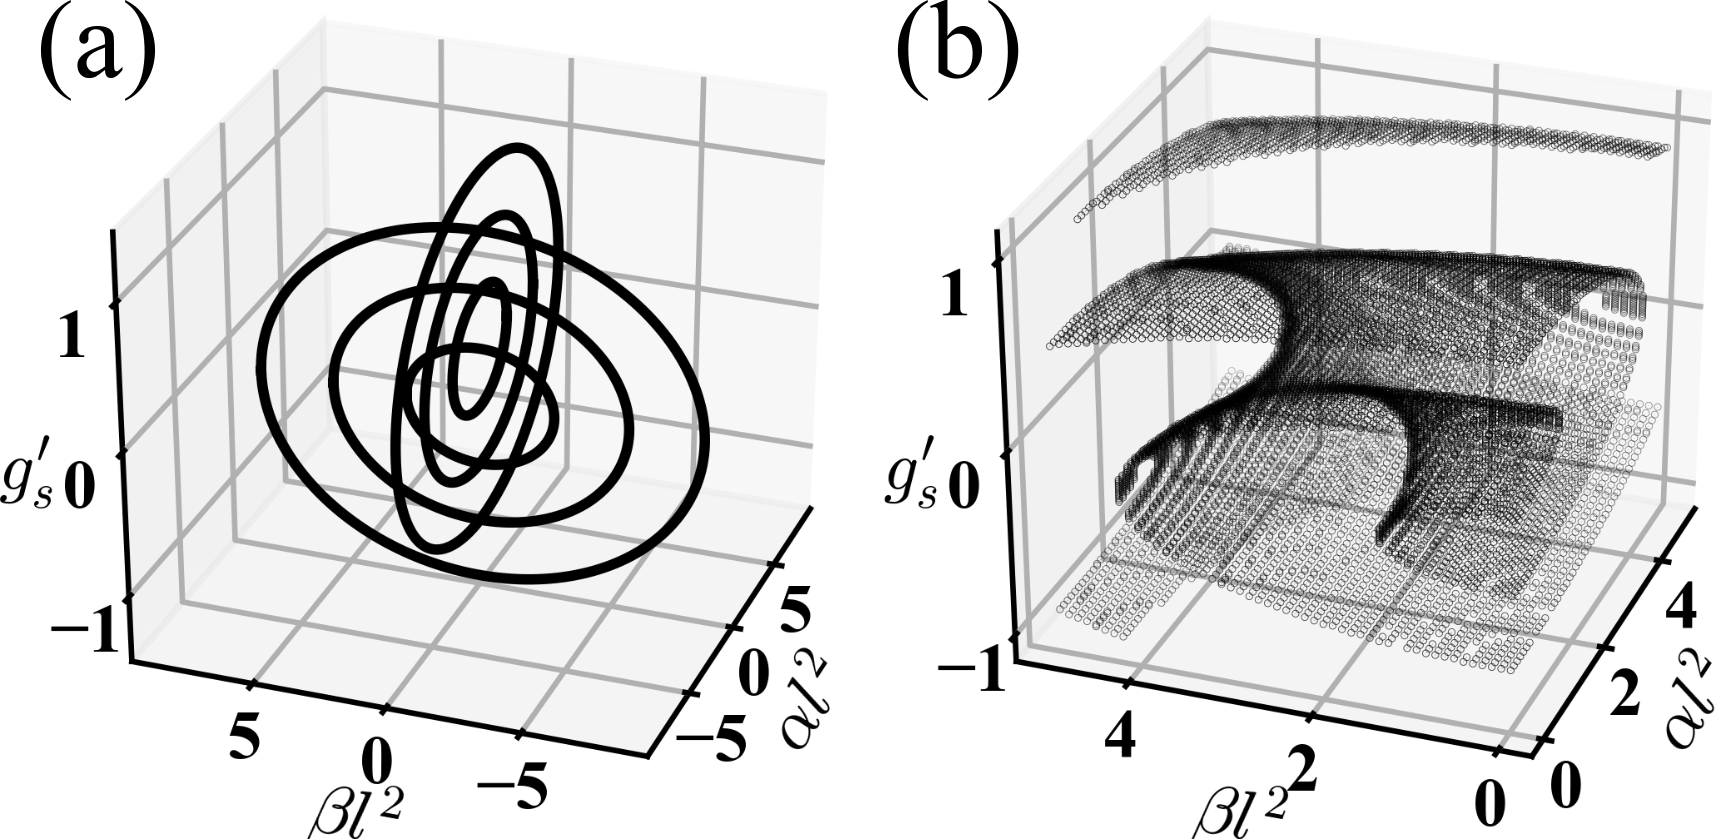
\includegraphics[width=1.0\columnwidth]{dgn.png}
\caption{Degenerate manifold of Rashba-Dresselhaus model. (a) degeneracy manifold of $\A=-I$; (b) degeneracy manifold of $\A=I$. Units: $\alpha l^2$($400$eV$\cdot$\AA$^3$), $\beta$($400$eV$\cdot$\AA$^3$), $g_s'$(10). Parameters are $m=0.01\hbar^2$/(eV$\cdot$\AA$^2$) and $E=0.4$eV. \red{[For 3D pictures, I always put units in caption since there's no room for them in the pictures.]}\label{fig:dgn}}
\end{figure}

The Rashba model suffers from an oversimplification -- continuous rotational symmetry is not a symmetry of solids. That is to say, it does not belong in any (magnetic) space group. It is possible for $\mathfrak{c}_{\infty}$-symmetric models to approximate Hamiltonians with a discrete, order-$n$ rotational symmetry (denoted $\mathfrak{c}_N$) \red{[Let's use capital N in $\mathfrak{c}_N$ since N coincides with order]}.  To what extent are Landau-level degeneracies (of $\mathfrak{c}_{\infty}$-symmetric systems) robust when $\mathfrak{c}_{\infty}$ is perturbatively reduced to $\mathfrak{c}_N$? Our general answer is out of every $N$ degeneracies of $\A$, $N-1$ of them are robust. \textbf{[results for n=3,4,6 must be checked]}. 

While full proof of the above claim is delegated to App. \ref{app:codimension}, let us illustrate the simplest example $N=2$ by introducing the Dresselhaus spin-orbit term ($\propto \beta$) into the Rashba model [cf.\ \q{hamRD}]. This has the desired effect of reducing $\mathfrak{c}_{\infty}$ to a discrete $\mathfrak{c}_2$ symmetry. Since $\A$ depends on $\alpha,\beta,l$ only through $\alpha l^2$ and $\beta l^2$, we consider the three-dimensional parameter space $(\alpha l^2,\beta l^2,g_s')\in \mathbb{R}^3$. If a  line node (in the $\beta{=}0$ plane) were perturbatively stable to finite $\beta$, then it would be embedded in a two-dimensional degeneracy hypersurface of $\mathbb{R}^3$; if the planar line node were unstable, this embedding does not happen, i.e., the planar line node is simply a line node in $\mathbb{R}^3$. Our numerical study shows that half the planar line nodes (corresponding to $\A{=}I$) are stable, while the other half ($\A{=}{-}I$) destabilizes. In $\mathbb{R}^3$, we then have pairs of line nodes and hypersurfaces enclosed by increasingly larger pairs of line nodes and hypersurfaces, as illustrated in Fig. \ref{fig:dgn}. 

To understand this pattern of stabilities, consider  the effective Hamiltonian $\calh$ in momentum independent basis (rather than spin-split basis used before)
\e{\calh=\alpha (k_{x}\sigma_{y}{-}k_{y}\sigma_{x})+\beta (k_{x}\sigma_{x}{-}k_{y}\sigma_{y})-\tf{g_s}{2}\mu_{B}B\sigma_z;}
with the Pauli matrices corresponding to spin operators. The two-fold rotational symmetry 
\e{\calh(\bk)=\sigma_z\calh(-\bk)\sigma_z, \;\: \bk(t)=-\bk\big(t+\tf{T_c}{2}\big)\in \frako_0,}
implies that the propagator over the time interval $[T_c/2,0]$ is symmetry-related to that over $[T_c,T_c/2]$:
\e{\A=\A_{T_c\leftarrow T_c/2}\A_{T_c/2\leftarrow 0}=\sigma_z{\A}_{T_c/2\leftarrow 0}\sigma_z {\A}_{T_c/2\leftarrow 0}.\la{eq:sigmazconstraint}}
The tracelessness of $\calh$ (at each $\bk$) implies that  ${\A}_{\sma{T_c/2\leftarrow 0}}$  has unit determinant. 
Utilizing the canonical parametrization for this $\text{SU}(2)$ matrix [Eq. (\ref{s3}) with ${\cal \bar{A}}$ replaced by ${\A}_{\sma{T_c/2\leftarrow 0}}$], we derive 
\e{
{\A}={\cal \bar{A}}=\matrixtwo{1{-}2R_2(R_2{-}iR_1)}{2iR_2(R_3{+}iR_4)}{{-}2iR_2(R_3{-}iR_4)}{1{-}2R_2(R_2{+}iR_1)} \label{proprashba}
}
with $\sum_{j=1}^4R_j^2{=}1$. We deduce from \q{proprashba} that $R_2{=}0$ is a necessary and sufficient condition for ${\cal \bar{A}}{=}I$. The corresponding degeneracy manifold is therefore a  unit-codimensional hypersurface which includes the free-electron limit: $\bR{=}(1,0,0,0)$. \red{[Discussion: I really hate introducing new symbols.]} \fig{fig:dgn}(b) illustrates the same hypersurface plotted with a different choice of coordinates: $(\alpha l^2,\beta l^2,g_s')$. On the other hand, ${\cal \bar{A}}{=}{-}I$ occurs if and only if $\bR{=}(0,1,0,0)$ -- a point in $\bR$-space. If $C_2$ were the only symmetry, then three parameters would be needed to tune ${\cal \bar{A}}{=}{-}I$. Generally, additional symmetry further constrains $\bR$, which may effectively reduce the number of tuning parameters.  This explains why the ${\cal \bar{A}}{=}{-}I$ manifolds, as plotted in Fig. \fig{fig:dgn}(a)], are line nodes instead of point nodes: these line nodes lie in either the $\alpha{=}0$ or the $\beta{=}0$ plane, both of which are $\mathfrak{c}_{\infty}$-symmetric.\footnote{To complete the explanation, \textbf{speculative:} the space of $C_{\infty}$-symmetric unitaries lie on lines in $\bR$-space that intersect $\bR{=}(0,1,0,0)$ [the point node]. A singular coordinate transformation to $\br$-space maps these $C_{inf}$-symmetric lines to $\mathfrak{c}_{inf}$-symmetric planes, and the point node to a line node.}


\subsection{Rotational symmetric magnetic breakdown}\la{sec:rotsymmbreakdown}

\begin{figure}
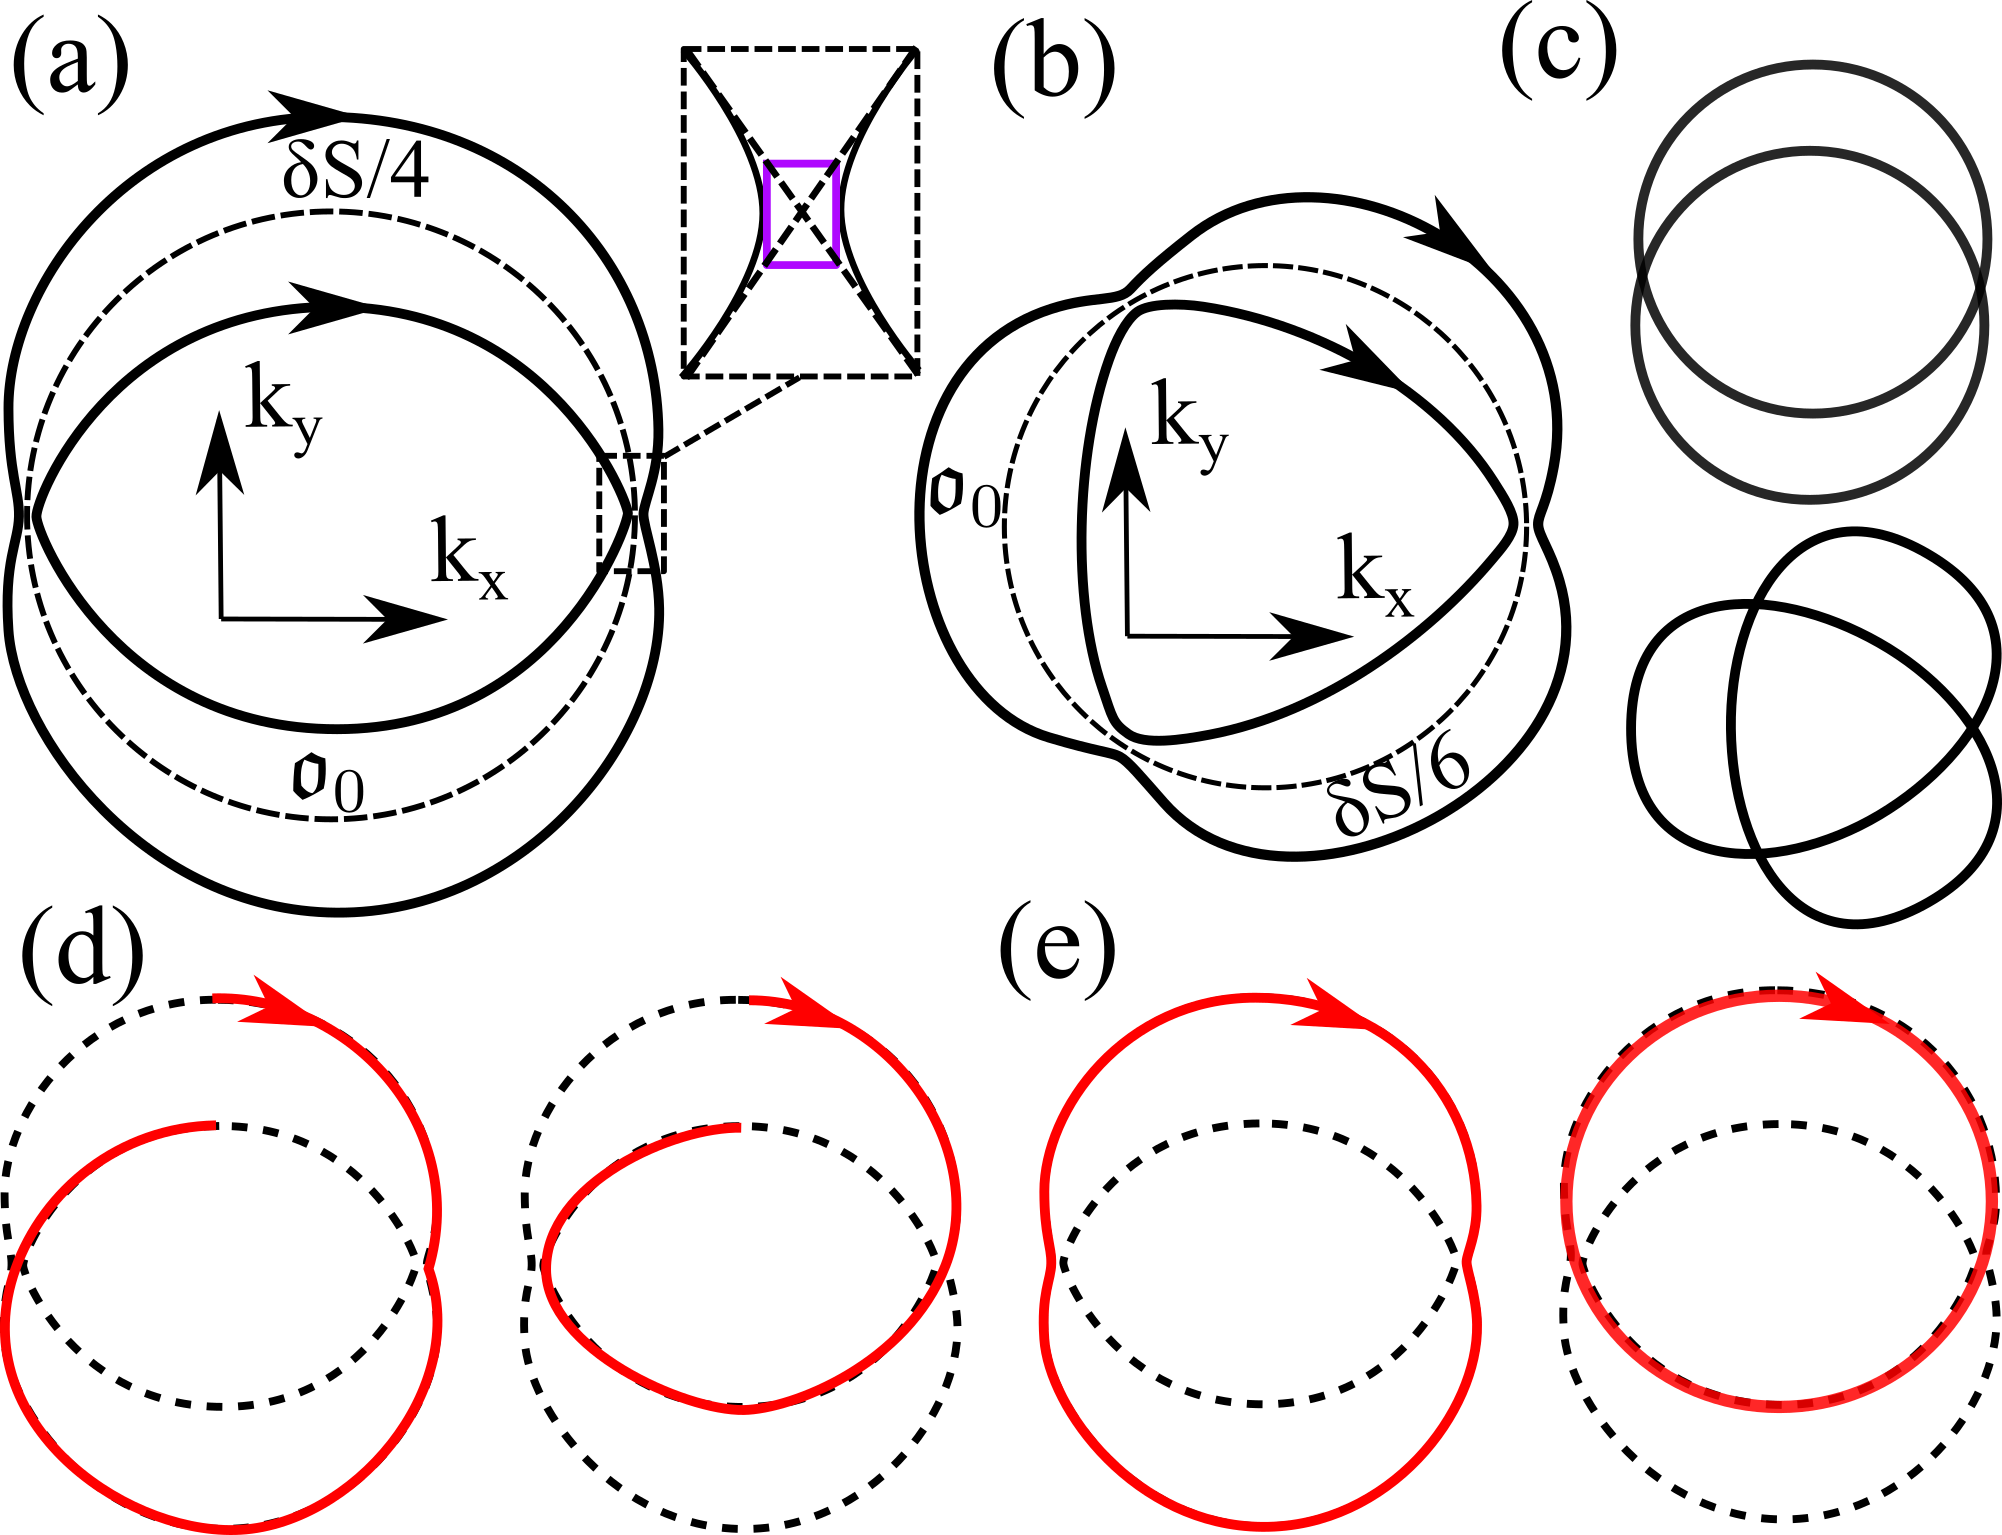
\includegraphics[width=1.0\columnwidth]{Cn-breakdown.png}
\caption{Cyclotron orbits for $\mathfrak{c}_2$-symmetric [(a)] and $\mathfrak{c}_3$-symmetric [(b)] breakdown. Bottom right inset of (a) presents an enlarged view of breakdown junction, where purple rectangle has area $S_{\sma{\square}}$.\label{fig:Cn-breakdown}}
\end{figure}

Quasidegenerate orbits feature tunneling everywhere along the cyclotron orbit and therefore demand a quantization rule that incorporates both tunneling and single band evolution of wave packets. Sometimes, the coherent evolution of wave packets and tunneling can be decoupled in the quantization rule in weak field limit, as exemplified by magnetic breakdown in Rashba-Zeeman model in Sec. \ref{sec:inplanezeeman}. Let us further explore single-parameter tunability of Landau-level quasidegeneracies in this limit by introducing a rotational symmetric Hamiltonian with isolated breakdown junctions at several isolated $\bk$ points. Besides being a useful toy model, this Hamiltonian provides some insights of stability of Landau-level quasidegeneracies by perturbing from two otherwise independent orbits.

We introduce a $\mathfrak{c}_2$-symmetric analog of the Rashba-Zeeman model:
\e{H=\f{\red{\hbar^2}k^2}{2m_1}+ \bigg(\f{\red{\hbar^2}k^2}{2m_2}-\mu\bigg)\sigma_z +wk_y\sigma_x,\la{modelC2breakdown}}
where $0<m_1{\ll}m_2,0<\mu$. For simplicity, we interpret the Pauli matrices as  spin operators, and the two right-most terms of  \q{modelC2breakdown} as a spin-orbit coupling. The $\mathfrak{c}_2$ symmetry manifests as $\sz H(\bk)\sz{=}H({-}\bk)$, and relates 
two Dirac points at
\e{\bar{k}_x = \pm\sqrt{2m_2\mu}/\red{\hbar},\;\bar{k}_y=0,\;\epsilon_{0}=\frac{m_2}{m_1}\mu.}
In the vicinity of either point, the  Hamiltonian has the linearized form 
\e{H_{\pm} =\pm \red{\hbar}\sqrt{\f{2\mu}{m_2}}\bigg(\frac{m_2}{m_1}+\sz\bigg)\delta k_x+w\delta k_{y}\sx+\epsilon_0, \la{linearHam2}}
from which we deduce that both Dirac points are  type-II if $m_1{<}m_2$; this condition is henceforth assumed.\footnote{Actually we will impose the stronger condition $m_1{\ll}m_2$, to ensure that the relative change in band velocity (due to the spin-orbit coupling) is small. This is a consistency requirement of our WKB theory, as explained in \app{app:quantizationruleproof}.} 

%; near each point the orbits are well approximated by two hyperbolic arms
%$\phi_j{=}\int_{\sma{0}}^{\sma{T_c}}\calh_{jj}dt/\hbar$ is simply the cyclotron integral of the corresponding diagonal element of the effective Hamiltonian. 

At energies close to the Dirac point ($E{-}\epsilon_0 {\ll} wm_2(2E/m_1)^{\sma{1/2}}$ \red{[need checking]}), there are two concentric orbits which (nearly) touch at both Dirac points, as illustrated in Fig. \ref{fig:Cn-breakdown} (a). Just as in \q{spinsplitwkb}, we define $\Delta$ as the spin-orbit splitting energy (averaged over the zeroth-order orbit with effective mass $m_1$). In the weak-field regime where $\var_c{=}\red{\hbar^2}/m_1l^2{\ll}\Delta$, interband tunneling is localized to the vicinities of the two II-Dirac points, and occurs with the Landau-Zener probability:
\e{\rho^2=e^{-2\pi\bar{\mu}}, \; \bar{\mu}=\f{\big(Z_{\perp}^2+(m_1/m_2)^2(E-\epsilon_0)^2\big)l^2}{2w\sqrt{2E/m_1}}. }
Elsewhere, a semiclassical wavepacket undergoes adiabatic (band-conserving) dynamics. For the upper half ($k_y>0$) of the diagram Fig. \ref{fig:Cn-breakdown}(a), this adiabatic evolution is described by a diagonal unitary matrix in the basis of energy bands; each diagonal entry encodes the slowly-varying semiclassical phase due to $\H$ ($\lambda_a'$ \red{[Let's use $\lambda_j'$ instead of $\delta_\lambda$. The latter is confusing because $\lambda_a\sim l^2 \delta S$. It would be quite confusing if we also let $\delta\lambda_a\sim l^2\delta S$]}) acquired along a spin-split trajectory to the \red{top}. In more detail, $\lambda_{\pm}'{=}{\pm}l^2\delta S/4$ up to a field-independent geometric phase \footnote{due to this field-independent phase, it is not necessary that $\delta\lambda_+=-\delta\lambda_-$}.  
The time-evolution propagator  describes the time-ordered, coherent process of interband tunneling (as described by the scattering matrix of \q{scattmat})
 and adiabatic dynamics:
\e{\A&=\red{e^{i(\lambda_+'+\lambda_-')}}\times\nonumber\\
&\left(\matrixtwo{\tau e^{i\bar{\varphi}}}{-\rho}{\rho}{\tau e^{-i\bar{\varphi}}}\red{\diagmatrix{e^{i\f{\lambda_+'-\lambda_-'}{2}}}{e^{i\f{\lambda_-'-\lambda_+'}{2}}}} \right)^2. \la{propC2breakdown}}
The two scattering matrices for both Dirac points are identical by $\mathfrak{c}_2$ symmetry; so are the two diagonal propagators corresponding to the left and right halves of the adiabatic dynamics. 

$\rho{=}0$  describes the adiabatic limit of two independent orbits with differential action $\delta S$. As described earlier in \s{sec:llquasideg}, degeneracies of $\cala$ occur with a periodicity (in $l^2$) of $2\pi/\delta S$, which corresponds to a periodic increment of a single flux quantum for  the differential magnetic flux (between the two spin-split orbits in real space). 
%The degeneracies alternate between $\cala{=}I$ and ${-}I$ on the B axis, hence the subset of degeneracies corresponding to $\cala{=}I$ (or ${-}I$) occur with a period of  $4\pi/\delta S$ (or two flux quanta).  

%occurs if and only if $\rho{=}0$ and  $\exp[i(\delta \lambda_+{+}\bar{\varphi})]$ is real, while 


Let us investigate the fate of these degeneracies as $\rho$ increases. While asymmetric interband tunneling generically destabilizes all degeneracies, we will demonstrate that two-fold-symmetric interband tunneling destabilizes only half of them. Indeed, the necessary condition for $\A\propto I$ is \e{\tau\cos(\f{\lambda_+'{+}\lambda_-'}{2}+\bar{\varphi})=\pm 1,0.\la{c2breakdowndgncondition}}
for $\rho{>}0$, only 0 in Eq. (\ref{c2breakdowndgncondition}) is possible, destabilizing half of the degeneracies. \footnote{Notice cosine function reaches 0 twice in a period}

Eq. (\ref{c2breakdowndgncondition}) with $0$ on the right hand side is the condition for destructive interference of the two Feynman paths that contribute to interband tunneling (as illustrated in \red{[Fig]}); this occurs with a period  of   $4\pi /\delta S$ (or two flux quanta). To appreciate this, consider that  for $(\lambda_+'{+}\lambda_-')/2$ to vary by $\pi$, $l^2$ must vary by $4\pi/\delta S$. On the other hand, the field dependence of the scattering phase is comparatively negligible: for $\bar{\varphi}(\bar{\mu})$ to vary  $\sim 1$, the Landau-Zener parameter $\bar{\mu}$ must vary by $\sim 1$;\footnote{See Fig.\ 10 in 100page} moreover, $2\pi\barmu{:}{=} (2\pi/8) l^2S_{\sma{\square}}$ with  $S_{\sma{\square}}$ the area of the rectangle inscribed between the two hyperbolic arms  (see inset of Fig. \ref{fig:Cn-breakdown} (a)); clearly $S_{\sma{\square}}{\ll}\delta S$.

%$2\pi\bar{\mu}{\sim}l^2 S_{\sma{\square}}/8$ where $S_{\sma{\square}}$ is much smaller than $\delta S$ [see inset of Fig. \ref{fig:Cn-breakdown}(a)].





%The periodicity (in $l^2$) of the destructive interference has a dual interpretation  in real space -- as a periodic increment of \textit{two} flux quanta for  the differential magnetic flux (between the two spin-split orbits).\footnote{To clarify, band-conserving orbits do not generically describe the dynamics -- except at fine-tuned fields associated to destructive interference of interband tunneling.} 


%This  provides yet another  illustration of the general statement proposed in \s{sec:singleparameterrashba}: due to two-fold rotational symmetry, half the degeneracies have unit codimension, and the other half has codimension two. 

An analogous model with $\mathfrak{c}_3$-related II-Dirac points  is illustrated in Fig. \ref{fig:Cn-breakdown}(b). The corresponding propagator $\A$ has a form analogous to \q{propC2breakdown} -- but with $(\cdot)^2$ replaced by $(\cdot)^3$, and with $\lambda_\pm'{=}\pm l^2\delta S/4$ replaced by $\pm l^2\delta S/6$ (plus a field-dependent geometric correction). The degeneracy condition is accordingly modified as $\tau\cos[(\lambda_+'{+}\lambda_-')/2{+}\bar{\varphi}]=\pm 1,\pm 1/2$. For nonzero tunneling ($\rho {>}0$), only $\pm 1/2$ is reachable where, of every three degeneracies that exist in the adiabatic limit ($\rho=0$), only two persist. $\tau=1/2$ marks a critical point where all degeneracies coalesce pairwise (on the $B$ axis) and annihilate. It is not hard to imagine the claim made in Sec. \ref{sec:singleparameterrashba} remains true: out of every $N$ degeneracies, $N-1$ of them are stable against $\mathfrak{c}_N$-symmetric breakdown (see App. \ref{app:codimension} for a proof).
%$\cala{=}{\pm} I$ is attained if and only if  $\tau \cos(\delta \lambda_+{+}\bar{\varphi}){=}{\mp}1/2$.

%There then are no more $B$-tunable degeneracies beyond a critical field where  $\tau{<}1/2$. 

%In the zero-tunneling limit ($\rho{=}0$), the condition for degeneracy (of $\cala$) is that $\exp[i(\phi_+{+}\bar{\varphi})]$ is a sixth root of unity -- the periodicity in $l^2$ corresponds to a single quantum of differential magnetic flux. 


\textbf{A different realization of two-fold symmetric breakdown: angular magnetoresistance oscillations.}
\red{[I begin to question this again. In my previous understanding, the in-plane magnetic field changes the band structure while the out-of-plane magnetic field produces LLs. Now I believe the in-plane magnetic field cannot be simply understood simply as a change in band structures. Therefore, I am not quite sure whether it is related to magnetic breakdown.]}

\subsection{The ten-fold table for symmetry constrained codimensions}\la{sec:tenfold}

\begin{table}
\begin{tabular*}{\columnwidth}{l@{\extracolsep{\fill}}ccccc}
\hlineB{2.0}
             & $u$ & $s$ & quasi. & $g$ & codim.\\
\hline
$\forall \bk \in \frako_0$, $g\circ \bk=\bk$ & 0 & 0 & $\surd$ & $\breve{g}\propto I$ & 3  \\
    &  &  & & $\breve{g}\not\propto I$ & 1 \\
    & 0 & 1 & & $g^2=1$ & 1  \\
    &  &  & & $g^2=-1$ & 3  \\
$|g\circ \frako_0| = |\frako_0|$ & 0 & 0 & $\surd$ & - & 1   \\
$\exists \bk \in \frako_0, g\circ \bk\ne\bk$    & 0 & 1 & & - & 1   \\
    & 1 & 0 & & $\breve{g} \propto \sigma_z$ & 2  \\
    &  &  & & $\breve{g} \not\propto \sigma_z$ & 0  \\
    & 1 & 1 & $\surd$ & $g^2=1$ & 2  \\
    &  &  & & $g^2=-1$ & 0  \\
$|g\circ \frako_0| \ne |\frako_0|$ & 0 & 0 & $\surd$ & - & 3 \\
    & 0 & 1 & & - & 3 \\
    & 1 & 0 & & - & 3 \\
    & 1 & 1 & $\surd$ & - & 3 \\
\hlineB{2.0}
\end{tabular*}
\caption{Codimensions of degeneracy manifold of two-by-two propagator $\A$ under constraints of different type of symmetries. The first column defines how the symmetry act on the cyclotron orbit, where $g\circ \bk$ (resp. $g\circ\frako$) is the image of $\bk$ (resp. $\frako$) under the the action of $g$. $|g\circ \frako=\frako|$ indicates the image of the orbit coincides with itself, regardless of orientation of the orbit. The next two columns are intrinsic properties of $g$. $u=0$ (resp. $u=1$) indicates the symmetry is a proper (resp. improper) transformation of the plane of the cyclotron orbit ($k_z=\text{constant}$). $g$ of $u=0$ (resp. $u=1$) does not flip (resp. flips) the orientation of the cyclotron orbit. $s=0$ (resp. $s=1$) indicates the symmetry is unitary (resp. antiunitary). In magnetic groups, antiunitary symmetry operations contain time reversal symmetry. The fourth column indicates whether this symmetry class applies to quasidegenerate propagator $\A$. For the five classes not applicable here, they are useful for Landau levels of fully degenerate bands, as discussed in Sec. \ref{sec:discussion}. The fifth column specifies additional conditions (on the representation of $g$) which are necessary to obtain a unique answer for codimension. $\breve{g}$ is the diagonalized, unitary matrix representation of $g$ in the degenerate subspace. The last column is codimension of the degeneracy manifold.\label{table:codimension}}
\end{table}

Sec. \ref{sec:singleparameterrashba} and \ref{sec:rotsymmbreakdown} illustrate that rotational symmetry imposes constraints on $\A$ and reduces codimension of its degeneracy manifold. This reduction of codimension is not limited to rotational symmetry.

Since magnetic field $B$ is applied externally, it does not change under the action of any symmetry operation. Hence any symmetry relevant in current context must keep $k_x$-$k_y$ plane untouched. By definition, $\A$ is a path-ordered exponential along the cyclotron orbit of the two-by-two Hamiltonian $\H$ and $\H$ is composed of a scalar $\delta\epsilon$ and a pseudovector $B\mathcal{M}$. Whether the symmetry $g$ transforms the cyclotron orbit to itself (denoted as $|g\circ\frako_0|=|\frako_0|$) or not ($|g\circ\frako_0|\ne|\frako_0|$) determines whether a self constraint can be imposed on $\A$. The former case can be again divided into two types, one for $g$ mapping every $\bk$ on the orbit to itself and one for at least one $\bk$ on the orbit being mapped to another point. Moreover, whether $g$ preserves the direction of cyclotron orbit (denoted as $u(g)=0$) or not (denoted as $u(g)=1$) indicates whether the path-order in $\A$ needs to be inversed. Besides the transformation of orbits, the transformation of $\H$ is also significant in determining the transformation of $\A$. As a scalar, $\delta\epsilon$ remains intact under the action of $g$ while in contrast $\mathcal{M}$ changes to $(-1)^{u+s}\mathcal{M}$, with $s(g)=0$ (resp. $s(g)=1$) denoting $g$ being unitary (resp. antiunitary). For $\H$ transforming consistently under $g$, $u+s=0, 2$ is required. The indicators defined above classifies symmetry operations into ten and only ten classes, presented in table \ref{table:codimension}.

With detailed codimension analysis delegated to App. \ref{app:codimension}, we present the result in table \ref{table:codimension}. To obtain a unique answer for codimension in some of the symmetry classes, we have to specify certain conditions for the symmetry representation: for $g$ that does not invert time ($s{=}0$), we specify certain conditions on  $\breve{g}$, the \emph{diagonalized} matrix representation  of $g$; for $g$ that inverts time  ($s{=}1$), we specify if the antiunitary representation of $g$ squares to $+I$ or $-I$.  Codimension 0, 1, 2 and 3 can be readily recognized in table \ref{table:codimension}. $T\mathfrak{r}_{x,\boldsymbol{c}/2}$ ($\mathfrak{r}_{x,\boldsymbol{c}/2}$ is glide plane translating in $z$ direction for half a lattice vector after flipping $x$ direction) at $k_z=\pi$ is an example of codimension 0, corresponding to class-6 (the 6th class in the table) \red{[Notice that I changed the name of the class. I begin to think class II-A bears more similarity to class-I and the original classification is not natural. Therefore, I abandoned the I, II-A and II-B. Do you agree?]} with condition $g^2=-1$. Due to similar reasons as Kramer's degeneracy, Landau-level quasidegeneracy are guaranteed for arbitrary parameter choice. Rotational symmetry belonging to class-3 has codimension 1, as confirmed by numerical study and arguments in Sec. \ref{sec:singleparameterrashba} and \ref{sec:rotsymmbreakdown}. Codimension 2 is exemplified by $T\mathfrak{r}_x$ ($\mathfrak{r}_x$ is reflection in $x$ direction) belong to class-6 with $g^2=1$. Class-1 symmetries with $\breve{g}\propto I$, acting effectively as identity operator, imposes no constraints on $\A$ and thus no reduction in codimension.


\textbf{[for classes with codimension less than three, please give physical intuition and examples of symmetries where possible. For example, I-1 with breveg not proportional to identity merely reflects that different representations of a unitary symmetry do not hybridize at any point along orbit. give mirror symmetry as example.]}

\red{[need to define stable or robust]} Codimension 1 does not imply every degeneracy is robust, which is a stronger statement than degeneracy manifold can be found by tuning a parameter. If degeneracy manifold contains distinct components of different codimension, every degeneracy being robust implies all these components having codimension 1, which is generally not the case, as exemplified by rotational symmetry discussed in Sec. \ref{sec:singleparameterrashba} and \ref{sec:rotsymmbreakdown}. Table \ref{table:codimension} only lists the smallest codimension, which is the number of parameters needed to find a degeneracy. 

%We end this section by a general discussion of free parameters that is most tunable in experiments. In transport experiments, magnetic field $B$ is generally tunable; in tunneling spectroscopy experiments, both $B$ and bias voltage $E$ is tunable. If codimension of degeneracy is 1, as constrained by two types of symmetries in Table \ref{table:codimension}, Landau level degeneracies can be found by tuning either $B$ or $E$. We have argued in Sec. \ref{sec:qtznrules} that $\lambda_a$ varies slowly with respect to $B$ and $E$. Hence an \textit{aperiodic} beating pattern is expected by tuning either $B$ or $E$.

\subsection{Magnetic quantum Oscillations}\label{sec:qo}

We have shown that by tuning a single parameter $B$, Landau level quasidegeneracies can be found for some symmetry classes. In this section, we study how Landau level quasidegeneracies are reflected on magnetic quantum oscillations and more generally, possible implications of $\lambda_a$ on the oscillation pattern.

Traditionally, quantum oscillations of thermodynamic and transport quantities are best understood for nondegenerate orbits in the absence of breakdown; they originate from the periodic (in $1/B$) depopulation of discrete Landau levels as $B$ is ramped up. For spin-degenerate orbits in the absence of breakdown, it is the depopulation of every second Landau level that is periodic. With magnetic breakdown at isolated points, the harmonic content of quantum oscillations generically includes multiple periods corresponding to distinct orbits. A distinctive feature of spin-split bands is that quantum oscillations are generically aperiodic. 

%In 2D electron systems, analysis of quantum oscillations is subtle since oscillations of the chemical potential may change the oscillating behaviour qualitatively. Therefore,

We will separately analyze the oscillations of two types of 2D electron systems distinguished by experimental environment: where (i) chemical potential is kept constant and (ii) particle density is kept constant. To analyze quantum oscillations in case (i), it is advantageous to have a Lifshitz-Kosevich-type formula so that Fourier-like components may be separately analyzed. Lifshitz-Kosevich formula have been derived in the absence of breakdown, and in the presence of magnetic breakdown at isolated points [Kaganov, lifshitz]; here we report that a Lifshitz-Kosevich formula also exists for coupled spin-split bands:\footnote{This formula corrects a factor of two in our previous work [topofermi].} In particular, for de Hass-van Alphen (dHvA) oscillation, the oscillatory component of the magnetization has the form
\begin{equation}
\delta M=-\frac{1}{2\pi}\frac{k_BT}{B}S\sum_{a=1}^D\sum_{r=1}^{\infty}e^{-\frac{r\pi}{\omega_c\tau}}\frac{\text{sin}[r(l^2S+\lambda_a+\gamma_a)]}{\text{sinh}(2\pi^2rk_BT/(\hbar\omega_c))},\label{eq:LK}
\end{equation}
where the argument of the sinuisoidal functions involve quantities from our generalized quantization rule, $T$ is temperature and $\tau$ is Dingle scattering lifetime. All the quantities on the right handside of Eq. (\ref{eq:LK}) are evaluated at Fermi energy. For 3D systems, Lifshitz-Kosevich formula is in a similar form, presented in Ref. [topoferm]. If temperature is large compared to the cyclotron frequency and/or $1/\tau$ is large, it is well-known that only the lowest harmonics ($r\sim 1$) are observable. If right handside of Eq. (\ref{eq:LK}) is contributed by two orbits, the most important oscillating part is the sum of two sine functions and $\lambda_a$ there determines whether the two sine functions are added constructively ($\delta \lambda=0$, corresponding to Landau level quasidegeneracy) or destructively ($\delta\lambda=\pi$). $\delta\lambda$ here is defined as $\delta\lambda:=|\lambda_1-\lambda_2| \mod 2\pi$. This interference phenomenon has been studied previously for spin splitting factor [topofermi], where $\lambda$ is field independent. For quasi-degenerate bands, $\lambda$ here is field dependent. Since $\lambda$ varies slowly with respect to magnetic field compared to leading term $l^2S$, a beating pattern is expected. Generically, $\delta \lambda$ nonlinearly depends on $l^2$, leading to an \textit{aperiodic} beating in the dHvA oscillation. Figure \ref{fig:qo} (a) shows the evolution of $\delta\lambda$ with respect to magnetic field for various parameters of Rashba-Dresselhaus system. Whenever $\delta\lambda$ reaches $\pi$ (resp. $0$), a beating node (resp. antinode) is expected. 

%surface states of 3D solids (insulators and metals, of both trivial and topological categories), as well as (ii) 2DEG in semiconductor heterostructures or 2D materials on substrates. Quantum oscillations of the chemical potential are generically negligible in case (i),

% \footnote{Suppose $\mu$ is the field-dependent chemical potential of a 3D solid with surface states. Since $\mu$ is an intensive quantity, it may be approximated by the chemical potential $\mu'$ corresponding to the same 3D solid but with periodic boundary conditions in three independent directions. If said solid is an insulator, $\mu'$ would depend smoothly on $B$; if said solid is a metal, the quantum oscillations of $\mu'$ have negligible amplitude so long as the Fermi surface is not highly anisotropic.[lifshitz,kosevich] } and non-negligible in case (ii).

As will be shown below, for quantum oscillations in case (ii), $\delta\lambda$ also governs the oscillation pattern. For concreteness we consider Schubnikov-de Haas (SdH) oscillations of the conductivity. With the assumption of constant particle density, period of quantum oscillation without magnetic breakdown is solely determined by particle number density $n_e$ as $e/n_eh$ [Vinter]. Minimum of conductivity occurs right at the point when one Landau level is completed depopulated, i.e., when the chemical potential jumps. However, these minimums may be smeared out by temperature or disorder. Whether the minimums are vulnerable to smearing depends on the Landau level gap, i.e., the magnitude of the jump of chemical potential. Larger Landau level gap prevents the conduction minimum from being smeared out and thus corresponds to oscillation of larger magnitude. This Landau level gap is governed by $\delta\lambda$. We plot in Fig. \ref{fig:qo} (b) lower panel chemical potential oscillation with respect to $1/B$ under the assumption of zero energy and zero Landau level broadening where $\delta\lambda{\approx}2\pi$, $\delta\lambda{\approx}3\pi/2$, $\delta\lambda{\approx}\pi$ respectively; the corresponding Landau-level dispersions are obtained from exact diagonalization and plotted in upper panel of Fig. \ref{fig:qo} (b). As expected, close to Landau level quasidegeneracy ($\delta\lambda\approx 0$), half of the oscillations are smeared out and the oscillation period has effectively doubled. This behavior is further confirmed by the oscillation of chemical potential plotted in lower left plot of Fig. \ref{fig:qo} (b). As a contrast, middle column of Fig \ref{fig:qo} (b) shows Landau levels and chemical potential oscillation for $\delta\lambda\approx 3\pi/2$, when quantum oscillation are expected to exhibit large and small oscillations. For $\delta\lambda\approx\pi$, the two sets of Landau levels are equally spaced and quantum oscillation are expected to reveal the particle density of the system. Therefore, for 2D fixed particle density systems, both oscillation period and oscillation magnitude are beating \textit{aperiodically} with respect to magnetic field.

It is well known that quantum oscillations from two independent cyclotron orbits (but with similar area in reciprocal space) may also exhibit periodic beatings. This is due to Landau levels corresponding to the two orbits may also cross approximately (with a splitting $\sim e^{-c/B}$). Such crossings are not so surprising, and merely reflect that distinct orbits are essentially uncoupled; this is very much analogous to the crossing of levels having different symmetry eigenvalues. In contrast, for weakly spin-split bands, the two orbits are strongly coupled by tunneling, hence there are no obvious `symmetry eigenvalues'; nevertheless crossings exist and are tunable by $B$. The hybridization of the two sets of Landau levels destroy the periodic nature of approximate crossings and is reflected in an \emph{aperiodic} beating pattern.
\textbf{
[We should say that experimental groups (e.g. Das) have already been fitting the beating in oscillations to cos(Laurent series in B), with phenomenological coefficients. Here we provide the microscopic derivation of these coefficients.  ]}

% Another distinction: for localized breakdown, crossings occur only at $B\approx 0$, while for nonlocal breakdown they recur aperiodically  at fields denoted $B_n$. The recurrence interval for $1/B_n$ is much larger than the period of quantum oscillations, leading to an aperiodic beating effect in the quantum oscillations.

\begin{figure}
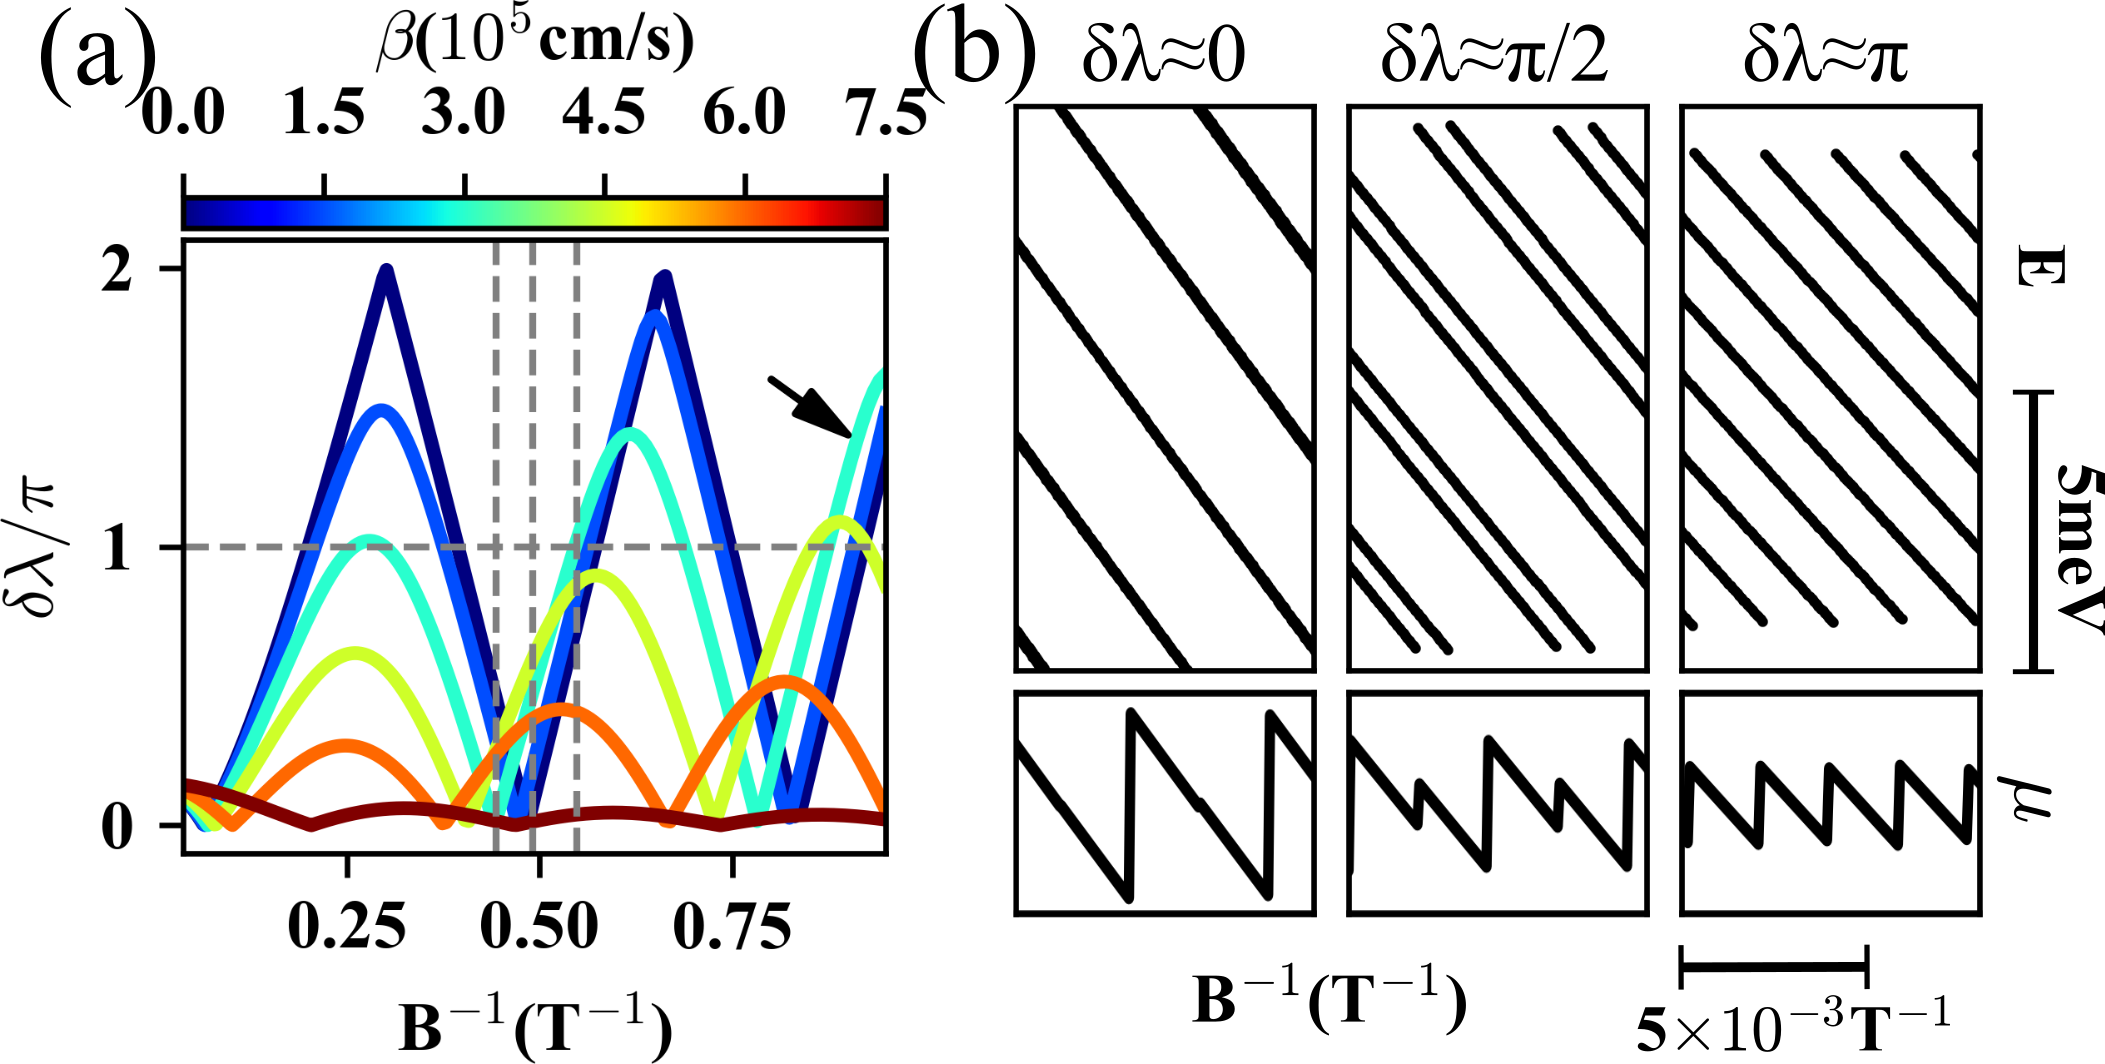
\includegraphics[width=1.0\columnwidth]{qo.png}
\caption{Quantum oscillation of Rashba-Dresselhaus system. (a) Evolution of $\delta\lambda$ with respect to field for different value of $\beta$. Horizontal grey lines are $\delta\lambda=\pi$. Upper panel of (b): Landau levels near fields indicated by vertical grey lines in right panel of (a) at $\beta=0.02$eV$\cdot$\AA, corresponding to $\delta\lambda=2\pi$, $\delta\lambda=3\pi/2$ and $\delta\lambda=\pi$ respectively. The line of $\beta=0.02$eV$\cdot$\AA~is indicated by a black arrow in (a). Lower panel (b): Oscillations of chemical potentials corresponding to upper panel. Fixed partical number density is assumed. In this figure, other parameters are $m=0.01$/(eV$\cdot$\AA$^2$), $\alpha=0.05$eV$\cdot$\AA~and $E=0.4$eV.
\label{fig:qo}}
\end{figure}

\section{Discussion and outlook}\la{sec:discussion}

Landau level quasidegeneracy is not limited to quasidegenerate bands. For degenerate bands, a similar definition is applicable: \red{[need to check]}
\e{ \f{E_{1}-E_2}{\var_c}\bigg|_{\bar{B}} = O\left(\f{\var_c}{E} \right). } Landau levels of degenerate bands are characterized by a propagator $\A'$ similar to Eq. (\ref{eq:prop}) [100p]. Codimension analysis can be carried out similarly and the results are presented in table \ref{table:codimension}. Unlike $\A$, all ten classes of symmetries impose constraints on $\A'$ and thus entries not applicable to $\A$ are useful for $\A'$. For spin-split bands, $\lambda$ depends strongly on the $B$ field for quasidegenerate orbits; for degenerate orbits, the $B$-dependence of $\lambda$ is relatively weaker, i.e., of higher power in the small parameter $B$ [Roth, Niu, Fuchs]. A more useful tuning parameter in the latter case would be the bias voltage in tunneling spectroscopy experiments. 

We have assumed in the above sections that the two-fold quasidegeneracy is due to small SOC. More generally, two-fold degenerate bands can be perturbed into quasidegenerate bands by symmetry breaking. From this viewpoint, our previous assumption of small SOC breaks continuous spin rotational symmetry which protects the degeneracy of spin up and spin down states. Other common symmetry operations capable of protecting two fold degeneracy are $T\mathfrak{i}$ and $T\mathfrak{c}_{2z,\boldsymbol{c}/2}$ at $k_z=\pi$, where $T$ is time reversal symmetry; $\mathfrak{i}$ is inversion symmetry and $\mathfrak{c}_{2z,\boldsymbol{c}/2}$ is two-fold screw rotation in $z$ direction. Table \ref{table:codimension} is applicable to quasidegenerate bands ($\A$) perturbed from degenerate bands protected by all the three symmetries and degenerate bands ($\A'$) due to $T\mathfrak{i}$ or $T\mathfrak{c}_{2z,\boldsymbol{c}/2}$. For degenerate bands protected by continuous spin rotation, codimension is at most 1 since $\A'$ is diagonal in spin basis. Codimension analysis without assumption of degenerate bands being protected by the three symmetries are presented in App. \ref{app:codimension}, where codimensions of Landau level quasidegeneracy for possibly fine tuned degenerate/quasidegenerate bands can be found.

\begin{table}
\begin{tabular*}{\columnwidth}{l@{\extracolsep{\fill}}ccc}
\hlineB{2.0}
 symmetry  & origin of degen. & $\breve{g}\propto$ \\
\hline 
 $\mathfrak{t} \mathfrak{r}_x^n \mathfrak{r}_z^m$ & $T\mathfrak{i}$ & $\sigma_z$ \\
  $\mathfrak{t} \mathfrak{r}_x^n \mathfrak{r}_z^m$ & continuous spin rotation & $\sigma_z$ \\
 $\mathfrak{r}_z$, $\mathfrak{r}_x$, $\mathfrak{r}_{x,\boldsymbol{c}/2}\mathfrak{r}_z$ & $T\mathfrak{c}_{2z,\boldsymbol{c}/2}$ & $I$ \\
$\mathfrak{r}_{x,\boldsymbol{c}/2}$, $\mathfrak{r}_x \mathfrak{r}_z$  & $T\mathfrak{c}_{2z,\boldsymbol{c}/2}$ & $\sigma_z$ \\
\hlineB{2.0}
\end{tabular*}
\caption{Two by two sewing matrices for reflections and glide planes. The second column specifies the origin of two fold degeneracy. Glide operation in $x$ or $y$ direction is irrelevant; for example, $\mathfrak{r}_x$ and $\mathfrak{r}_{x,\boldsymbol{b/2}}$ share the same entry. $x$ and $y$ are equivalent; for example, $\mathfrak{r}_x$ and $\mathfrak{r}_y$ share the same entry. $\mathfrak{t}$ is (arbitrary) translation. When the two-fold degeneracy is protected by $T\mathfrak{c}_{2z,\boldsymbol{c}/2}$, $k_z=\pi$ is assumed.\label{table:sewing-matrix}}
\end{table}

Table \ref{table:codimension} has introduced diagonalized representation matrix $\breve{g}$ and has used it to obtain a definite answer for codimension for some classes. Fortunately, in most cases, $\breve{g}$ can be calculated without knowing the wave functions of the bands. In addition, symmetry operations whose sewing matrices are needed are mostly reflections (for example, reflection in $x$ direction $\mathfrak{r}_x$) and glide planes (for example, $\mathfrak{r}_{x,\boldsymbol{c}/2}$ where $\boldsymbol{c}$ is lattice vector in $z$ direction). Therefore, for convenience, we presented in table \ref{table:sewing-matrix} sewing matrix for common reflections, glide planes and combination of them. In most scenarios, given the space group, table \ref{table:codimension} and \ref{table:sewing-matrix} are adequate to determine the codimension of Landau level quasidegeneracy.

% Our conclusion that spin-degenerate Landau levels may be obtained by tuning a single parameter  may seem to contradict a theorem by Wigner and von Neumann that states the codimension of degeneracies of a complex Hermitian matrix is three; in our context this matrix is the Peierls-Onsager Hamiltonian whose spectrum corresponds to Landau levels. This theorem leads to the famous ``no-crossing rule" in physics, which states that generically there are no crossings of energy levels of Hamiltonians defined over  one- or two-dimensional parameter spaces. To reconcile our findings with this theorem, one should recognize that any energy level obtained from a semiclassical quantization rule is only asymptotically accurate (in powers of $B$, and the spin-orbit coupling). A degeneracy obtained from this approximation scheme may in principle be split on a scale of order $\var_c^2/E$ or $\var_c\var_s/E$; in principle, the approximation can be improved order by order. This distinction between asymptotically-accurate and exact degeneracies  affords a reconciliation with the Wigner-von Neumann theorem, but should  not typically be resolvable in experiments  due to the broadening effects of  temperature and disorder-induced scattering. 

\textbf{[comment on higher-order-in-B corrections to lambda, which will lead at ultra-high fields to landau-level quasidegeneracies]}

%In summary, we have developed a theory to calculate landau levels in the case of quasidegenerate orbits. This theory is asymtotically correct with small $k$ space splitting and works equally well if there are band touchings between the two quasidegenerate orbits. Aperiodic beating pattern in quantum oscillation is predicted to be observed in such systems.


\begin{acknowledgments}

We are grateful to Nicholas Read and Judith H\"oller for clarifying notions related to codimensions of matrix degeneracies. 
We acknowledge support by  the Yale Postdoctoral Prize Fellowship (AA), NSF DMR Grant No.\ 1603243 (LG),  the Ministry of Science and Technology of China, Grant No.\ 2016YFA0301001 (CW and WD), and the National Natural Science Foundation of China, Grants No.\ 11674188 and 11334006 (CW and WD). This work was performed in part at Aspen Center for Physics, which is supported by National Science Foundation grant PHY-1607611.
\end{acknowledgments}

\bibliography{paper}

%\part{Supplementary Material}

\appendix

\section{Review of effective Hamiltonian}\label{app:revieweffham}

Effective Hamiltonian lies in the heart of semiclassical theory. The leading order term (with respect to $B$) of effective Hamiltonian in momentum representation can be obtained by Peierls substitution of crystal momentum $\boldsymbol{k}$: $\boldsymbol{k}\to\boldsymbol{K}=\boldsymbol{k}+\frac{e}{\hbar}\boldsymbol{A}(i\nabla_{\boldsymbol{k}})$ in zero field band structure $H_{0}(\boldsymbol{K}):=\epsilon(\boldsymbol{k})$, where $\boldsymbol{A}$ is vector potential. Components of $\boldsymbol{K}$ do not commute with each other, thus substituting $\boldsymbol{k}$ to $\boldsymbol{K}$ is performed in a Weyl-symmetric manner that can be formally done using Fourier transformation. Wave functions in momentum representation are represented as $\phi=\sum_{\boldsymbol{k}}f_{\boldsymbol{k}}\psi_{\boldsymbol{k}}$, where $\psi_{\boldsymbol{k}}$ is modified Bloch wave function whose specific form is presented in [Roth]. The effective Hamiltonian then acts on $f_{\boldsymbol{k}}$, changing Shr\"odinger equation to:
\begin{equation}
(H(\boldsymbol{K})-E)f_{\boldsymbol{k}}=0.\label{eq:schrodinger}
\end{equation}
Subleading order term of effective Hamiltonian $H_{1}(\boldsymbol{K})$ is also obtained by substituting $\boldsymbol{k}$ to $\boldsymbol{K}$ in $H_{1}(\boldsymbol{k})$, where $H_{1}(\boldsymbol{k})$ encodes information of non-Abelian Berry phase, orbital magnetization and Zeeman energy. Assuming a magnetic field $B$ in $-z$ direction,
\begin{equation}
H_{1}(\boldsymbol{k})=eB\epsilon^{\alpha\beta}\mathfrak{X}^{\beta}v^{\alpha}+BM^{z}-g\mu_{B}B\sigma^{z}
\end{equation}
where $[\mathfrak{X}^{\alpha}]_{nm}=i\langle u_{n\boldsymbol{k}}|\partial_{k^{\alpha}}u_{m\boldsymbol{k}}\rangle$ is Berry connection, $[v^{\alpha}]_{nm}=\frac{1}{\hbar}\delta_{nm}\partial_{k^{\alpha}}\epsilon$ is band velocity, $M^{z}$ is orbital magnetization, $g\approx 2$ is the free-electron g-factor and $\mu_{B}$ is the Bohr magneton. Eq. (\ref{eq:schrodinger}) can be solved by WKB approximation. To the leading order, solution of Eq. (\ref{eq:schrodinger}) is Zilberman function
\begin{equation}
f_{k}=\frac{c}{\sqrt{|v^{x}|}}e^{ik_{0}^{x}k^{y}l^{2}}e^{-il^{2}\int k^{x}dk^{y}}\delta_{k_{0}^{x}k^{x}},
\end{equation}
where $c$ is an arbitrary constant and the integration is performed along constant energy contours. $k^x$ is a constant of motion in Landau gauge, which is why a $\delta_{k_{0}^{x}k^{x}}$ appears in Zilberman function.

\section{Proof of quasi-degenerate quantization rule\label{app:quantizationruleproof}}

\textbf{Give some motivation for why we might care about quasidegeneracy greater than two. E.g, new fermions, accidental degeneracies, mirror planes??}

Since $\delta S=0$ without $\alpha\mathcal{W}$, $\alpha$ is proportional to $\delta S$ up to linear order. A good example is Rashba Hamiltonian in the main text, where $\delta S=4\pi m\alpha\sqrt{2m\epsilon}+\text{O}(\alpha^2).$  Thus 
\begin{equation}
\mathcal{H}=
\mathcal{H}_0+\delta S \mathcal{W}'+\text{O}(\delta S^2),
\end{equation}
where $\delta S \mathcal{W}'=\alpha \mathcal{W}$.
We seek a generalized quantization condition of the form 
\begin{equation}
l^{2}S+\lambda_{a}+\gamma=2\pi n.
\end{equation}
In previously-studied quantization rules for non-degenerate and degenerate band subspaces, $\lambda$ is field-independent and of order one. The additional small parameter in quasi-degenerate magnetotransport allows to formulate a dimensionless quantity that is of order one: $l^2\delta S$. We therefore posit a field-dependent $\lambda$ that is  of order $\text{O}(1,l^2\delta S)$.

To obtain a quantization rule up to order $\text{O}(1,l^2\delta S)$, we need to formulate an effective Hamiltonian that is accurate to $\text{O}(l^{-2},\delta S)$.  Following the
idea of [Roth], it is not difficult to verify this effective Hamiltonian for a specific band is 
\begin{align}
H &= H_{0,0}+H_{1,0}+H_{0,1}+\text{o}(l^{-2}, \delta S),\\
H_{0, 0}&=\epsilon_0(\boldsymbol{K}),\\
[H_{0, 1}]_{nm}&=\delta S [\mathcal{W}'(\boldsymbol{K})]_{nm} = \alpha [\mathcal{W}(\boldsymbol{K})]_{nm},
\end{align}
where $\epsilon_0$ is band dispersion of $\mathcal{H}$ and $H_{1,0}(\boldsymbol{k})$ is still Eq. (\ref{eq:H1}) evaluated in the absence of $\alpha\mathcal{W}$. $\text{o}$ here is small-o notation

We now group the  terms in effective Hamiltonian as $\tilde{H_0}=H_{0,0}$ and $\tilde{H}_{1}:=H_{1,0}+H_{0,1}$. The Schr\"odinger equation is now
\begin{equation}
(\tilde{H}_{0}(\boldsymbol{K})+\tilde{H}_{1}(\boldsymbol{K})-E)f=\text{o}(l^{-2}, \delta S).
\end{equation}
Similar to what is done in [100page], we seek the solution to the Schr\"odinger equation using superposition\textbf{[strange way to put it]} of Zilberman-Fischbeck functions
\begin{equation}
\boldsymbol{f}=A\boldsymbol{f}^{0},
\end{equation}
where 
\begin{equation}
f_{a}^{0}=c_{a}\frac{1}{\sqrt{|v_0^{x}|}}e^{ik_{0}^{x}k^{y}l^{2}}e^{-il^{2}\int k^{x}dk^{y}}\delta_{k_{0}^{x}k^{x}}.
\end{equation}
$A$ is a square matrix with the assumption $A_{ab}$ is of order $O(1,l^2\delta S)$. Following section V of [100page], we have:
\begin{widetext}
\begin{equation}
[H_{0}(\boldsymbol{K})]_{ab}A_{bc}f_{c}^{0}=A_{ac}\epsilon_0(\boldsymbol{K})f_{c}^{0}+il^{-2}\partial_{y}A_{ac}\hbar v_0^{x}f_{c}^{0}+\text{o}(l^{-2}, \delta S),
\end{equation}
and
\begin{equation}
[\tilde{H}_{1}(\boldsymbol{K})]_{ab}A_{bc}f_{c}^{0}=[\tilde{H}_{1}]_{ab}A_{bc}f_{c}^{0}+\text{o}(l^{-2}, \delta S).
\end{equation}
\textbf{[Let's clarify at what wavevector tildeH1 is supposed to be evaluated. Let's also write out explicitly the next order term in B10, which is proportional to the spin-orbit-induced change in the band velocity. At two points in the paper, I said that the relative change in velocity must be small, so here it will be justified. ]}
\end{widetext}

Sch\"rodinger equation then becomes 
\begin{equation}
il^{-2}\partial_{y}A_{ac}\hbar v^{x}f_{c}^{0}+[\tilde{H}_{1}]_{ab}A_{bc}f_{c}^{0}=\text{o}(l^{-2}, \delta S).
\end{equation}
We want the above equation to hold for any $\mathbf{c}$, so 
\begin{equation}
\hbar\partial_{y}A_{ac}=il^{2}[v^{x\nu}]^{-1}[\tilde{H}_{1}]_{ab}A{}_{bc},
\end{equation}
thus
\begin{equation}
A=\overline{\text{exp}}[il^{2}\int\frac{\tilde{H}_{1}}{\hbar v_0^{x}}dk^{y}].
\end{equation}
$\lambda_{a}$ are again given by eigenphases of propagator $A$ along a complete orbit
\begin{equation}
\mathcal{A}[\mathfrak{o}]=\overline{\exp}[il^{2}\oint_{\mathfrak{o}}\frac{\tilde{H}_{1}}{\hbar v_0^{x}}dk^{y}].
\end{equation}


\section{Consistency conditions for our quantization rule}\la{sec:slowvariation}


The following are consistency conditions for our quantization rule:
\e{ |l^2S| \gg |\lambda_a|,\, \left|l^2\p{S}{E}\right| \gg \left|\p{\lambda_a}{E}\right|,\, \left|S\right| \gg \left|\p{\lambda_a}{l^2}\right|.} 
Due to the latter two inequalities, we shall refer to $\lambda_{a}$ as \textit{slowly-varying} (with respect to $E$ and $B$), in comparison with the rapidly-varying $l^2S$. To appreciate the difference in scales, consider that for $\lambda_a$ to change by $2\pi$ due to a variation $l^2$ (at fixed energy), we estimate [in the weak-field regime; cf.\ \q{phaseindependentorbit}] that $l^2$ must change on the scale of $2\pi/\delta S$; this scale is much greater than the period of quantum oscillations ($T_{1/B}{:}{=}2\pi/ S$), by our assumption of quasidegeneracy. Analogously, for $\lambda_a$ to vary by $2\pi$ due to a variation of $E$ (at fixed field) by $\delta E$, we estimate [from \q{phaseindependentorbit}] that $\delta E {\sim} 2\pi/l^2 (\partial \delta S/\partial E)$, which is generically much larger than the cyclotron energy $\epsilon_c{=}2\pi/l^2 (\partial  S/\partial E)$. In the strong-field regime (where $\delta \var$ may be neglected from \q{eq:H1}), $\lambda_a$ is independent of $B$ (to the accuracy of our semiclassical theory\textbf{[add footnote to describe higher order corrections]}), and depends on $E$ solely through the slow variation of $\calm$.  In the absence of symmetry, we  estimate 
\e{\p{\lambda_{a}}{E}=\order\left(\f{g_s}{m_0}\p{m}{E},\f{\partial^2S/\partial E^2}{\partial S/\partial E} \right)\ll \f{2\pi}{\var_c},} 
where $\order(a,b)$ is defined as the order of magnitude of either $a$ or $b$ (whichever is larger), $m_0$ is the free-electron mass, and $m{=}\hbar^2(\partial S/\partial E)/2\pi$ the effective mass. The first argument of $\order$ originates from the energy dependence of the effective g-factor (with $g_s$ the free-electron g-factor, and $m/m_0$ the dimensionless effective mass); the second argument accounts for possible non-analyticities in the area of $\frako_0$, which may originate from saddle- or II-Dirac points in the zeroth-order band Hamiltonian.




\section{Existence of Landau-level quasidegeneracy}\la{sec:proofLLquasideg}


This appendix demonstrates that, if a degeneracy of $\cala$ [$e^{i\lambda_+}{=}e^{i\lambda_-}$] occurs at $(\bar{E},\bar{B})$, there exists two Landau levels in close proximity to $(\bar{E},\bar{B})$ which satisfy the quasidegeneracy conditions defined in \qq{llquasideg}{llquasidegB}.

To begin, it is useful to define
\e{ \calq_{\pm}(E,B):= \f1{2\pi}\left(l^2S +\lambda_{\pm} -\gamma \right)}
such that the quantization rule \q{eq:rule} is satisfied if $\calq_{\pm}(E,B){\in}\Z$. 
Generically, either of $m_{\pm}:=\calq_{\pm}(\bar{E},\bar{B})\in \R$ is not integer-valued, but 
\e{\big(\calq_{+}-\calq_{-}\big)\bigg|_{\bar{E},\bar{B}}=\f{\lambda_+-\lambda_-}{2\pi}\bigg|_{\bar{E},\bar{B}} \in \Z. \la{diffinteger}} 
Let $n_{\pm}$ be the closest integer to $m_{\pm}$ (this implies $|n_{\pm}-m_{\pm}|<1$).  From \q{diffinteger}, we deduce that $n_+-m_+$ is equal to $n_--m_-$; this quantity is henceforth denoted as $r:= n_{\pm}-m_{\pm}$, and  $\calq_{\pm}(\bar{E},\bar{B}){+}r{\in} \Z$. 

Let us first tackle \q{llquasideg}. We define $E_{\pm}$ such that $\calq_{\pm}(E_{\pm},\bar{B}){=}\calq_{\pm}(\bar{E},\bar{B}){+}r{\in} \Z$. Since  $\lambda_{\pm}$ is a slowly varying function of $E$ relative to $l^2S$, $|E_{\pm}{-}\bar{E}|/\var_c{\approx} |r|{<}1$, with the cyclotron energy $\var_c=2\pi/l^2|\partial S/\partial E|$ evaluated at $(\bar{E},\bar{B})$. Let us denote $O':=\partial O/\partial E$ evaluated at $(\bar{E},\bar{B})$. We estimate
\e{\f{E_+-E_-}{\var_c} \approx &\; \f{r}{\var_c}\left(\f1{\calq'_+}-\f1{\calq'_-}\right)\approx  \f{r}{2\pi}\var_c \left( \lambda'_- -\lambda'_+\right). \la{estimate}}
What is left is to estimate $\lambda_{\pm}'$, which we have accomplished in \s{sec:qtznrules} in both weak- and strong-field regimes. Combining our estimates for $\lambda'$ with \q{estimate}, we  arrive at \q{llquasideg}.

%From \s{sec:qtznrules}, we know that for sufficiently weak field ($\var_c\ll \Delta$), $\lambda_{\pm}'\approx \pm l^2\delta S'/2$. For $\var_c\gg \Delta$, $\lambda_{\pm}'$ is determined by the energy dependence of the field-dependent terms in the effective Hamiltonian $\calh$.  

Let us next tackle \q{llquasidegB}. It is most convenient at this point to change variables from $B\rightarrow l^2$ (the square of the magnetic length). Let us  define   $l^2_{\pm}$ such that $\calq_{\pm}(\bar{E},l^2_{\pm}){=}\calq_{\pm}(\bar{E},l^2_{\pm}){+}r{\in} \Z$. We denote  $\dot{O}:=\partial O/\partial(l^2)$ evaluated at $(\bar{E},\bar{B})$, and estimate
\e{\f{l^2_+-l^2_-}{T_{\sma{1/B}}} \approx  \f{r }{2\pi}T_{\sma{1/B}} \left( \dot{\lambda}_- -\dot{\lambda}_+\right)=O\left(\f{\delta S}{S}\bigg|_{\bar{E}}\right). \la{estimateB}}
The order-of-magnitude estimate is obtained in the limit $\var_c\ll \Delta$, where $\lambda_{\pm}\approx \pm l^2\delta S/2$ [cf.\ \q{phaseindependentorbit}]. In the opposite limit $\Delta\gg \var_c$, $\lambda_{\pm}$ is independent of $B$ within the accuracy of our semiclassical theory.    

\section{Codimension of Landau level quasidegeneracy}\la{app:codimension}

In this appendix, we expose mathematical details of symmetry analysis of the quasidegenerate propagator $\A$ and derive symmetry constrained codimension of degeneracy manifold. We restrict our analysis to two-by-two $\A$.

\begin{table*}[t]
\begin{tabular*}{2\columnwidth}{l@{\extracolsep{\fill}}ccccccc}
\hlineB{2}
             & $u$ & $s$ & symmetry constraint & $\det{\A}$ & $\breve{g}$ & codimension \\
\hline
(I) $\forall \bk \in \frako$, $g\circ \bk=\bk$ & 0 & 0 & $\A=\breve{g}\A\breve{g}^{-1}$ & - & $\breve{g}\propto I$ & 3  \\
&  &  &  & - & $\breve{g} \not\propto I$ & 1  \\
& 0 & 1 & $\A=\breve{g}\A^*\breve{g}^{-1}$ & 1 & $(\breve{g}K)^2=I$ & 1 \\
&  &  &  & 1 & $(\breve{g}K)^2=-I$ & 3 \\
&  &  &  & -1 & $(\breve{g}K)^2=I$ & $\infty$ \\
&  &  &  & -1 & $(\breve{g}K)^2=-I$ & $\times$ \\
(II-A) $|g\circ \frako| = |\frako|$ & 0 & 0 & $\A=\breve{g}(g^{L-1}\circ\bk_0)\prod_{i=0}^{L-1} \A_{1/L}$ & - & - & 1 \\
$\exists \bk \in \frako, g\circ \bk\ne\bk$ & 0 & 1 & $\A=\breve{g}(g^{L-1}\circ\bk_0)\prod_{i=0}^{L-1} K^i\A_{1/L}K^i$ & - & $L=N$ & 1 \\
& & & & 1 & $L\ne N$ & 1 \\
& & & & -1 & $L\ne N$, $(\breve{g}K)^2=I$ & $\infty$ \\
& & & & -1 & $L\ne N$, $(\breve{g}K)^2=-I$ & $\times$ \\
& 1 & 0 & $\A=\breve{g}\A^\dagger\breve{g}^{-1}$ & 1 &$\breve{g} \propto \sigma_z$& 2\\
& & & & 1 &$\breve{g} \not\propto \sigma_z$ & 0\\
& & & & -1 &$\breve{g} \propto I$ & 2\\
& & & & -1 &$\breve{g} \not\propto I$& 0\\
& 1 & 1 & $\A=\breve{g}\A^T\breve{g}^{-1}$ & - & $(\breve{g}K)^2=I$ & 2 \\
& & & & - & $(\breve{g}K)^2\ne I$ & 0 \\
(II-B) $|g\circ \frako| \ne |\frako|$ & 0 & 0 & $\A_2=\breve{g}\A_1\breve{g}^{-1}$ & - & - & 3 \\
& 0 & 1 & $\A_2=\breve{g}\A_1^*\breve{g}^{-1}$ & - & - & 3\\
& 1 & 0 & $\A_2=\breve{g}\A_1^\dagger\breve{g}^{-1}$ & - & - & 3\\
& 1 & 1 & $\A_2=\breve{g}\A_1^T\breve{g}^{-1}$ & - & - & 3 & \\
\hlineB{2}
\end{tabular*}
\caption{ \textbf{[for II-A-1, you might replace product with a power, and breveg by a phase factor; it looks a little disconcerting that L-1 is specially chosen in the argument. ]} Codimensions of degeneracy manifold of $\A$ or $\A'$ under constraints of different type of symmetries. Most of the symmetry constraints on $\A$ are reproduced from Ref. [100p] except for the first two classes in type II-A, where a special gauge is chosen. $\infty$ in the codimension column denotes that eigenvalues of $\A$ cannot be degenerate; $\times$ denotes an entry where we cannot self-consistently impose the symmetry constraint and the conditions on det$\A$ and $\breve{g}$ for a two-by-two unitary $\A$. In the second to last column, $\breve{g}$ is either chosen to be diagonal or off-diagonal \label{table:fullcodimension}}
\end{table*}

Since direction of external magnetic field is fixed (pointing to $-z$ direction in our convention), only symmetry operators mapping $z$ to $\pm z$ are relevant for cyclotron orbits. These symmetry operators can be classified into ten and only ten classes [100p]. The classification is based several indicators of symmetry operator $g$, namely $u(g)=0~(1)$ representing $g$ is a proper (improper) rotation of the cyclotron orbit and $s(g)=0~(1)$ representing $g$ is unitary (antiunitary). However, unlike Ref. [100p], only five out of ten symmetry classes impose constraints on $\A$. This reduction of relevant symmetry classes is due to components of $\calh$ transforming differently under symmetry operations. $\delta\epsilon$ transforms as a scalar but orbital moment and spin transforms as a pseudovector. The five symmetry classes are tabulated in Table \ref{table:codimension} in the main text. Here we calculate codimension of degeneracy manifold for all the ten classes since the other five classes are relevant for quantization rule of degenerate bands.

Sewing matrix is necessary to express the constraints on the propagator $\A$. \red{For a symmetry operator $\hat{g}$ acting on wave functions as $\hat{g}|\psi(\br)\rangle=|\psi(g^{-1}\br)\rangle$ [Really need to introduce $\check{g}$?]}, the sewing matrix $\breve{g}$ is defined as 
\e{
   \breve{g}_{nm} = \langle u_{n,g\circ\bk}|\hat{g}(\bk)|u_{m,\bk} \rangle K^{s(g)}.
}
Here, $K$ is complex conjugation; $\hat{g}(\bk)=e^{-i\bk\cdot\hat{\br}}\hat{g}e^{i\bk\cdot\hat{\br}}$; $g\circ\bk$ is the image of $\bk$ under the action of $g$; $n$ and $m$ \textbf{[m=1,2,n=1,2]} runs over the degenerate subspace. Diagonalized representation matrix of unitary $\hat{g}$ introduced in the main text is sewing matrix in a special gauge, so we use the same symbol $\breve{g}$. \textbf{[introduce what this gauge freedom is, and what are gauge-invariant quantities]}

Sewing matrix is needed to express symmetry constraints since there is an ambiguity in choosing the basis of degenerate subspace. Therefore, it can be drastically simplified if a good basis is chosen. \textbf{[give equation for how breveg is transformed with a different gauge choice]} Generally, we have the following rules for two-by-two sewing matrix:
\begin{itemize}
\item If $g\circ\bk\ne\bk$, $\breve{g}(\bk)$ can be transformed into identity matrix by a gauge transformation.
\item If $g\circ\bk=\bk$ and $\hat{g}$ is unitary, $\breve{g}(\bk)$ can be transformed into a diagonal matrix by a gauge transformation.
\item If $g\circ\bk=\bk$ and $\hat{g}$ is antiunitary, $\breve{g}(\bk)$ can be transformed into an off-diagonal matrix (diagonal terms are 0) by a gauge transformation.  For the special case of $\hat{g}$ that is order-2, $\breve{g}$ can be transformed into either $\sigma_z$  or $i\sigma_y$. We define order $N$ of $g$ as the smallest positive integer fulfilling $g^N$ is identity, $2\pi$ rotation, lattice translation or products of them. \textbf{[this definition of order should be moved up to above paragraphs where you introduce basic manipulations of sewing matrix]}
\end{itemize}
The first two claims are obvious \textbf{[it's only obvious once you give the equation for gauge-transform of breveg]} and the last claim can be verified by a direction calculation showing diagonal terms can be eliminated by a gauge transformation no matter what $\breve{g}$ is at the beginning. \textbf{[add this last proof in separate appendix]}

The symmetry constraints on $\A$ expressed using sewing matrix is presented in Ref. [100p] and reproduced in Table \ref{table:fullcodimension} for convenience. Generally, these constraints are derived using the following relation
\e{
&\A[g\circ \bk_f\leftarrow g\circ \bk_i] \nonumber\\
&=e^{i\phi}\breve{g}(\bk_f)K^{s(g)}\A[\bk_f\leftarrow \bk_i]K^{s(g)}\breve{g}^{-1}(\bk_i),\label{eq:propsymm}
}
\textbf{[define K to the power]} where $\A[\bk_f\leftarrow \bk_i]$ is a segment of the propagator from $\bk_i$ to $\bk_f$ along the cyclotron orbit. $e^{i\phi}$ is a phase factor that appears for $g$ that is a nonsymmorphic element; however this phase always drops out[100page] for closed orbits and will be neglected in the subsequent analysis.

For four of  the ten classes (class II-B), the symmetry relates the propagators of distinct and disconnected orbits, but each propagator (corresponding to one orbit) is itself unconstrained.  Therefore, the codimensions are still 3 \textbf{[must be careful in presentation, how do we distinguish orbit degeneracies from the spin degeneracies that is the focus of this work]}. For the other six classes, a case by case study is needed. 

The symmetry constraints in Table \ref{table:fullcodimension} can be divided into two types: (i) the first two rows of class II-A and (ii) other rows. For symmetry constraints of type (i), the full propagator is decomposed into products of $L$ (whose meaning will be explained below) segments of the propagator. These segments are related to one another by sewing matrix. Therefore, we parametrize the first segment of the propagator $\A_{1/L}$ as
\e{
\A_{1/L} = e^{i\theta}\matrixtwo{\alpha}{\beta}{-\beta^*}{\alpha^*}, |\alpha|^2+|\beta|^2=1.\label{eq:paramA1/N}
}
Then we calculate the full propagator $\A$ and figure out how many parameters is needed to tune $\A$ such that $\A$ is proportional to identity, which is codimension of degeneracy manifold. For symmetry constraints of type (ii), $\A$ fulfills an equation expressed with sewing matrix at the base point of $\A$ (denoted as $\bk_0$). Therefore, we parametrize the propagator as
\e{
\A = e^{i\theta}\matrixtwo{\alpha}{\beta}{-\beta^*}{\alpha^*}, |\alpha|^2+|\beta|^2=1.
}
and look for how many free parameters are left after the symmetry constraint is imposed, which is codimension of degeneracy manifold.


\paragraph*{class I-1} According to the general rules of sewing matrix, the sewing matrix $\breve{g}$ can be made diagonal by a gauge transformation
\e{
\breve{g} = \matrixtwo{e^{i\phi_1}}{0}{0}{e^{i\phi_2}}.
}
In this gauge, the symmetry constraints are expressed as 
\e{
\matrixtwo{\alpha}{\beta}{-\beta^*}{\alpha^*}=\matrixtwo{\alpha}{e^{i(\phi_1-\phi_2)}\beta}{-e^{-i(\phi_1-\phi_2)}\beta^*}{\alpha^*}.
}
Therefore, unless $\breve{g}$ is proportional to identity, $\beta=0$ and the only free variable is the phase of $\alpha$.

\paragraph*{class I-2}
By a gauge transformation, the sewing matrix $\breve{g}$ can be made off-diagonal
\e{
\breve{g} = \matrixtwo{0}{1}{\pm 1}{0}.
}
In this gauge, the symmetry constraints are expressed as (notice that $\det(\A)=\pm 1$ in this class \textbf{[this should not be inserted as a casual remark, please formalize]})
\e{
\det({\A})\matrixtwo{\alpha}{\beta}{-\beta^*}{\alpha^*}=\matrixtwo{\alpha}{\mp\beta}{\pm \beta^*}{\alpha^*}.
}
This immediately gives corresponding rows in table. \ref{table:fullcodimension}.

\paragraph*{class II-A-3 and class II-A-4} Calculation of codimensions for the two classes follow the same pattern as class I and is therefore omitted here.

\paragraph*{class II-A-1} In this class \textbf{[not just this class, also II-A-2]}, the full propagator can be constructed from $1/L$ of it, where $L$ is the smallest positive integer fulfilling $g^L\circ \bk_0=\bk_0$. Here, $\bk_0$ is the base point of $\A$. In this class, $L=N$. A good example in this class is $\mathfrak{c}_{Nz}$, $N$-fold rotation in z direction.\textbf{ [give the more general expression first before you perform your gauge transform]} Generally, by gauge transformation at $g^n\circ \bk_0$, $\breve{g}(g^n\circ \bk_0)$ can be transformed to identity for $0 \le n < N-1$ and the full propagator is
\e{
\A=\breve{g}(g^{N-1}\circ\bk_0)\prod_{i=0}^{N-1} \A_{1/N}
}
where 
\e{
\breve{g}(g^{N-1}\circ\bk_0)=\prod_{n=0}^{N-1} \breve{g}(g^n\circ\bk_0)
}
is a constant phase factor determined by the group multiplication rule. For example if $g$ is an $N$-fold rotation,  the phase factor is $+1$ (resp.\ $-1$) for an integer-spin (resp.\ half-integer-spin) representation. Therefore, the central object is
$\prod_{i=0}^{N-1} \A_{1/N}$. We take $N=2$ as an example. Using the parametrization in Eq. (\ref{eq:paramA1/N}),
\e{
\A_{1/N}^2=e^{2i\theta}\matrixtwo{\alpha^2-|\beta|^2}{\beta(\alpha+\alpha^*)}{-\beta^*(\alpha+\alpha^*)}{\alpha^{*2}-|\beta|^2}.
}
For $\A_{1/N}^2 \propto I$, the sufficient and necessary condition is $\text{Re}(\alpha)=0,\pm 1$, where tuning $\text{Re}(\alpha)=0$ requires only one parameter while tuning $\text{Re}(\alpha)=\pm 1$ requires three parameters.

For crystallographic spacetime symmetries, $N$ may also equal 3, 4 or 6. It is straightforward to prove in a similar manner that in these cases, degeneracies of $\A$ lie at $\text{Re}(\alpha)=\cos(n\pi/N)$, with $n\in\mathbb{Z}$. Except for $\text{Re}(\alpha)=\pm 1$, all degeneracy manifolds have codimension 1. In the Sec. \ref{sec:llquasideg}, we construct $\mathfrak{c}_N$ models by perturbing from $\mathfrak{c}_\infty$ Rashba model and by coupling two otherwise independent orbits by magnetic breakdown. In both constructions, $\A_{1/N}$ can be written in some gauge choice as
\e{
	\A_{1/N}=e^{i\theta}\matrixtwo{e^{i\lambda}}{0}{0}{e^{-i\lambda}}
}
before perturbation is turned on. $\lambda$ evolves monotonically with respect to $B$ and sweeps through $n\pi/N$ where degeneracies of $\A$ are expected. $e^{i\lambda}$ hits $\pm 1$ once in every $N$ degeneracies and therefore the other $n-1$ degenerates are stable, i.e., have codimension 1.

\paragraph*{class II-A-2} In class II-A-1, $L=N$ is guaranteed. However, in class II-A-2, this is generally not true. For symmetry operations still respecting $L=N$, the codimension calculation is similar to what is done in class II-A-1. The only example of $L\ne N$ is $T\mathfrak{c}_{6z,n\boldsymbol{c}/6}$ ($n\in{0,1,2,3,4,5}$), where $L=3$ and $N=6$. We write $g=T\mathfrak{c}_{6z,n\boldsymbol{c}/6}$ and $h=g^3$. By gauge transformation, it is possible to make $\breve{g}(\bk_0)=\breve{g}(g\circ\bk_0)=I$ and $\breve{h}(\bk_0)=\breve{g}(g^2\circ \bk_0)\equiv\breve{h}$. In this gauge, $\breve{h}(g\circ\bk_0)=h^*$. Therefore,
\e{
\A=\breve{h}\A_{1/L}\A_{1/L}^*\A_{1/L}
}
and $\A_{1/L}$ is constrained due to $h$ as 
\e{
\A_{1/L}=\breve{h}^* \A_{1/L} \breve{h}^{-1}.\label{eq:TC6A1/L}
}
Since $h$ is of order two, $\breve{h}$ can either be chosen as $\sigma_x$ or $i\sigma_y$. Then we immediately get $\det \A_{1/L} = \pm 1$. We first study the case $\breve{h}=\sigma_x$. If $\det \A_{1/L} = 1$, we parametrize $\det \A_{1/L}$ as in Eq. (\ref{eq:paramA1/N}) with $\theta=0$. From Eq. (\ref{eq:TC6A1/L}), we get $\beta=0$ and thus 
\e{
\A = \matrixtwo{0}{\alpha^*}{\alpha}{0}
}
and eigenphases of $\A$ are fixed to $0$ and $\pi$. If $\det{\A_{1/L}}=-1$, $\theta=\pi/2$ in Eq.(\ref{eq:paramA1/N}) and we obtain
\e{
\A = \matrixtwo{\beta^{*3}}{0}{0}{\beta^3}
}
and the codimension is 1. If $h=i\sigma_y$, from the fourth entry of class I-2, we deduce $\det \A_{1/L}=1$. Choosing the parametrization in Eq. (\ref{eq:paramA1/N}) with $\theta=0$, we compute the codimension to be 1.

In the main text, we focus on degenerate bands whose degeneracy is protected by continuous spin rotational symmetry (i.e., no SOC) or antiunitary symmetry $g$ with $g\circ \bk=\bk$ and $g^2=-1$. For the former case, we have argued in the main text that $\det{\A}=1$ if $\det{\A}$ is quantized; for the latter case, we have presented in table \ref{table:fullcodimension} $\det{\A}=1$ (Notice $g$ belongs to class I-2). Therefore, we safely ignore $\det{\A}=-1$ entries in table \ref{table:fullcodimension} and obtain table \ref{table:codimension} in the main text. \textbf{[more general argument?:  if we’re concerned with spinful orbits, and in symmetry classes where u+s=1, delta var is traceless, hence det A=+1.]
}
\section{Two-by-two sewing matrix of antiunitary symmetry operator can be made off-diagonal}

We parametrize $\breve{g}$ as
\begin{equation}
\breve{g}=e^{i\theta}\left(\begin{array}{cc}
\alpha & \beta\\
-\beta^{*} & \alpha^{*}
\end{array}\right),
\end{equation}
and $V$ by
\begin{equation}
V=e^{i\phi}\left(\begin{array}{cc}
a & b\\
-b^{*} & a^{*}
\end{array}\right),
\end{equation}
\begin{widetext}
then 
\begin{align}
\breve{g} & \to V^{\dagger}\breve{g}V^{*}\\
 & =e^{i(\theta-2\phi)}\left(\begin{array}{cc}
a^{*} & -b\\
b^{*} & a
\end{array}\right)\left(\begin{array}{cc}
\alpha & \beta\\
-\beta^{*} & \alpha^{*}
\end{array}\right)\left(\begin{array}{cc}
a^{*} & b^{*}\\
-b & a
\end{array}\right)\\
 & =e^{i(\theta-2\phi)}\left(\begin{array}{cc}
a^{*2}\alpha+a^{*}b\beta^{*}-a^{*}b\beta+b^{2}\alpha^{*} & a^{*}b^{*}\alpha+bb^{*}\beta^{*}+aa^{*}\beta-ab\alpha^{*}\\
\cdots & \cdots
\end{array}\right).
\end{align}
\end{widetext}
Parametrizing $a=a_{1}+ia_{2}$, $b=b_{1}+ib_{2}$, $\alpha=\alpha_{1}+i\alpha_{2}$
and $\beta=\beta_{1}+i\beta_{2}$, we first remove the imaginary part
of $a^{*}b^{*}\alpha+bb^{*}\beta^{*}+aa^{*}\beta-ab\alpha^{*}$. If
we take both $a$ and $b$ to be real, we want
\begin{align*}
0 & =2ab\alpha_{2}-b^{2}\beta_{2}+a^{2}\beta_{2}\\
2ab\alpha_{2} & =(b^{2}-a^{2})\beta_{2}\\
2b\sqrt{1-b^{2}}\alpha_{2} & =(2b^{2}-1)\beta_{2}.
\end{align*}
This is always possible since $2b\sqrt{1-b^{2}}/(2b^{2}-1)$ can take
any real value for $b\in[-1,1]$. Therefore, we can safely assume
$\beta$ is real since a preliminary transformation can remove its
imaginary part. Then we want
\begin{align*}
0 & =a^{*2}\alpha+a^{*}b\beta^{*}-a^{*}b\beta+b^{2}\alpha^{*}\\
(a_{1}-ia_{2})^{2}(\alpha_{1}+i\alpha_{2}) & =-(b_{1}+ib_{2})^{2}(\alpha_{1}-i\alpha_{2})\\
(a_{1}^{2}-a_{2}^{2}-2ia_{1}a_{2})(\alpha_{1}+i\alpha_{2}) & =-(b_{1}^{2}-b_{2}^{2}+2ib_{1}b_{2})(\alpha_{1}-i\alpha_{2}).
\end{align*}
Real and imaginary part of the above equation are
\[
(a_{1}^{2}-a_{2}^{2})\alpha_{1}+2a_{1}a_{2}\alpha_{2}=-(b_{1}^{2}-b_{2}^{2})\alpha_{1}-2b_{1}b_{2}\alpha_{2}
\]
and 
\[
(a_{1}^{2}-a_{2}^{2})\alpha_{2}-2a_{1}a_{2}\alpha_{1}=(b_{1}^{2}-b_{2}^{2})\alpha_{2}-2b_{1}b_{2}\alpha_{1}.
\]
Therefore
\[
\frac{\alpha_{2}}{\alpha_{1}}=-\frac{(a_{1}^{2}-a_{2}^{2})+(b_{1}^{2}-b_{2}^{2})}{2a_{1}a_{2}+2b_{1}b_{2}}=\frac{2a_{1}a_{2}-2b_{1}b_{2}}{(a_{1}^{2}-a_{2}^{2})-(b_{1}^{2}-b_{2}^{2})},
\]
equivalent to
\[
|a|=|b|=\frac{\sqrt{2}}{2}
\]
and 
\[
\frac{\alpha_{2}}{\alpha_{1}}=-\frac{(a_{1}^{2}-a_{2}^{2})+(b_{1}^{2}-b_{2}^{2})}{2a_{1}a_{2}+2b_{1}b_{2}}.
\]
This can always be satisfied. For example, we can always take $b=1/2+i/2$
and the above equation becomes
\[
\frac{\alpha_{2}}{\alpha_{1}}=\frac{(2a_{2}^{2}-1/2)}{2a_{2}\sqrt{1/2-a_{2}^{2}}+1/2},
\]
which is always possible since $\frac{(2a_{2}^{2}-1/2)}{2a_{2}\sqrt{1/2-a_{2}^{2}}+1/2}$
can take any value.


\section{Method of numerical diagonalization}\la{sec:numerical}

The techniques for solving $\mathcal{H}_R(\bK)$ in \textbf{[eq]} is standard, but we describe it here since it is also used in numerical diagonalization of other Hamiltonians below with no closed analytic solutions. This technique relies on the fact that the commutation relation $[K_x,K_y]=il^{-2}$ bears similarity to that of position operator and momentum operator of simple harmonic oscillators. Therefore, $K_x$ and $K_y$ can be organized into creation and annihilation operators
\begin{align}
\begin{split}
K_x=&l^{-1}(a+a^\dagger)/\sqrt{2},\\
K_y=&-il^{-1}(a-a^\dagger)/\sqrt{2}.
\end{split}
\end{align}
Under this transformation, $\mathcal{H}_R(\bK)$ is transformed to
\begin{align}
\begin{split}
\mathcal{H}_{R}(\boldsymbol{K})=&\frac{1}{ml^2}(a^{\dagger}a+\frac{1}{2})
\\&+\sqrt{2}\alpha l^{-1}\left(\begin{array}{cc}
0 & -ia^{\dagger}\\
ia & 0
\end{array}\right)
-\frac{g_s'\sigma^z}{4ml^2},
\end{split}\label{eq:Rashba-ho}
\end{align}
where Zeeman coupling is already added. Eq. (\ref{eq:Rashba-ho}) have solutions in the form of $(c_1|n+1\rangle,c_2|n\rangle)$ where $c_1$ and $c_2$ are some constants and $|n\rangle$ labels the eigenstate of $a^\dagger a$.

\textbf{[combine this with above]
}Electron spectrum of this Hamiltonian in magnetic field is not exactly solvable to our knowledge. Yet multiband Peierls substitution is still applicable and the system can still be mapped into two coupled harmonic oscillators similar to Eq. (\ref{eq:Rashba-ho}). This Hamiltonian is infinite dimensional and can be diagonalized by cutting off at a high occupation number. 


\section{Dimension of degeneracy manifolds}\la{app:nullity}

Any $SU(2)$ matrix can be expressed as ${\cal \bar{A}}= e^{i\br\cdot \bsigma}$ with $\br=(x,y,z)$ a real three vector and $\bsigma=(\sigma_x,\sigma_y,\sigma_z)$ the vector of Pauli matrices. The condition for degeneracy can be expressed as
\e{ 0=D^{\pm}=\det[{\cal \bar{A}}\pm I] = 2(1\pm \cos r)\in \R, \as r:=|\br|. \la{semipos}}
Parametrizing  ${\cal \bar{A}}(\bR)$ with $\bR$ a real $d$-vector, we define the partial derivatives
\e{  D^{\pm}_j:= \p{D^{\pm}}{ R_j}\in \R, \as D^{\pm}_{ij}:= \p{^2D^{\pm}}{ R_i\partial R_j} \in \R.  }
$D^{\pm}_{ij}$, also known as the Hessian matrix, is real and symmetric. 

Let us prove that $D^{\pm}_j$ vanishes (for all $j$) when evaluated on the degeneracy manifold.  We express $D^{\pm}$ as the characteristic polynomial det$[{\cal \bar{A}}-\zeta I]$ evaluated at $\zeta=\mp 1$:
\e{ D^{\pm}(\bR)=c_0(\bR)(\mp 1-\zeta_1(\bR))(\mp 1-\zeta_2(\bR)) }
where $\zeta_j$ are the unimodular eigenvalues of ${\cal \bar{A}}$. In this form it is clear that
the first derivatives of $D^{\pm}$ vanish when $\zeta_1=\zeta_2=\pm 1$.

To alternatively derive the vanishing of $D^{\pm}_j$ where $D^{\pm}{=}0$, we may apply that  $D^{\pm}\in [0,4]$ [derived from \q{semipos}]. As an implication, consider a small displacement $\delta \bR$ away from  a point $\bR_0$  on the degeneracy manifold $D^{+}=0$:
\e{ D^+(\bR_0+\delta \bR)\eq  \f1{2} \sum_{i,j=1}^d\delta R_i D^{+}_{ij}(\bR_0) \delta R_j + O(\delta R_i^3) \lin 
\eq \f1{2}\sum_{j=1}^d c^2_j h_j + O(\delta R_i^3).\la{taylor}} 
Since $D^{\pm}$ is a semipositive definite function, it must be that $\sum_{ij}\delta R_i D^{+}_{ij}(\bR_0) \delta R_j\geq 0$ for any $\delta \bR$, i.e., the Hessian must be semipositive definite on the degeneracy manifold. In the last equality of \q{taylor}, we decomposed $\delta \bR=\sum_jc_j\bv_j$ into the real, orthonormal eigenvectors $\bv_j$ of $D^{+}_{ij}(\bR_0)$ with corresponding real eigenvalues $h_j$; note $h_j\geq 0$. We see that if $\bR_0+\delta \bR$ lies on the degeneracy manifold (i.e., $D^+(\bR_0+\delta \bR)=0$),  $\delta \bR$ must lie in the null space of $D^{+}_{ij}(\bR_0)$. This implies that the dimension of the degeneracy manifold is bounded by the dimension of this null space (i.e., the nullity).

To illustrate these degeneracy manifolds for $\bR=\br=(r_1,r_2,r_3)$ a real three-vector, and $\hat{r}_i:=r_i/r$ 
\e{ D^{\pm}_j = \mp 2\sin (r) \hat{r}_i, \as D^{\pm}_{ij}= \f{\sin r}{r}\big(\delta_{ij}-\hat{r}_i\hat{r}_j\big)+\hat{r}_i\hat{r}_j\cos r.}
The degeneracy manifolds are given by $r=n\pi$ with $n\in \Z$. In particular, $D^{\pm}_{ij}(\bze)$ is the identity matrix, which is consistent with $n=0$ manifold being a point; $D^{\pm}_{ij}(\pi,0,0)$ is a diagonal matrix with only a single nonzero entry ($-1$), which is consistent with the $n=1$ manifold being a two-sphere.
\section{Reducing nonlocal magnetic breakdown to local magnetic breakdown}
We take Rashba-Zeeman model as an example, revealing that quantization rule for nonlocal magnetic breakdown, in the limit of $\Delta\gg\epsilon_c$, becomes quantization rule for local magnetic breakdown.

In the limit of $\Delta\gg\epsilon_c$, the two orbits become nondegenerate everywhere except for the type II Dirac point. It is natural to decompose the propagator into two parts
\begin{equation}
\A = \A_2\A_1,
\end{equation}
where $\A_1:=\A[t_-\leftarrow t_+]$ encodes information of cyclotron motion from leaving the vicinity of the Dirac point (denoted as $t_+$) to entering the vicinity of the Dirac point again (denoted as $t_-$) and $\A_2:=\A[t_+\leftarrow t_-]$ encodes information of cyclotron passing the vicinity of the Dirac point. Notice that we have written down $\A$ (and $\A_1$, $\A_2$) in constant basis since $\calh$ diverges near the Dirac point if expressed in the energy band basis. $t_+-t_-\ll T_c$ due to the smallness of the Dirac point. A gauge transformation expresses $\A_1$ in the energy basis
\begin{equation}
V_+^\dagger\A V_+ = V_+^\dagger\A_2V_-V_-^\dagger\A_1V_+,
\end{equation}
where $V_\pm=V(\bk(t_\pm))$. We emphasize that while $V_-^\dagger\A_1V_+$ can be understand as $\A_1$ in energy basis, $V_+^\dagger\A_2V_-$ cannot due to the divergence of single band Berry connection at Dirac point. Since $\Delta\gg\epsilon_c$, diagonal terms of $\A_1$ is much larger than off-diagonal terms such that to the lowest order off diagonal terms can be neglected. Therefore, 
\begin{equation}
\A_1\approx\matrixtwo{\delta \Omega_1}{0}{0}{\delta \Omega_2},
\end{equation}
where $\delta\Omega_{1(2)}$ is the semiclassical phase accumulated from $t_+$ to $t_-$ besides $l^2 S$ by the two bands.


The other part $\mathcal{S}:=V_+^\dagger\A_2V_-$ is a standard Landau-Zener problem, as will be shown below. In the constant basis, 
\begin{equation}
\calh(t)=\alpha(k_{x}\sigma_{y}-k_{y}\sigma_{x})+Z_\parallel\sigma_{y}-Z_\perp\sigma_{z},
\end{equation}
where $k_x=-k_F \cos(\omega_c t)$ and $k_y=k_F \sin(\omega_c t)$. Since $t_+-t_-\ll T_c$, we can keep only the linear terms in $t$,
\begin{equation}
\calh(t)\approx\alpha k_F \omega_c t\sigma_x+(Z_\parallel-\alpha k_F)\sigma_y-Z_\perp\sigma_z.
\end{equation}
It is now obvious that $\mathcal{S}$ is a Landau-Zener problem: $\alpha k_F \omega_c t\sigma_x$ is linear in time; $(Z_\parallel-\alpha k_F)\sigma_y-Z_\perp\sigma_z$ is time independent; columns of $V_-$ and $V_+$ are approximately eigenvectors of $\sigma_x$. Therefore, $\mathcal{S}$ takes the form of a magnetic junction scattering matrix with
\e{\mu=\frac{ml^2(Z_\perp^2+(Z_\parallel-\alpha k_F)^2)}{2\alpha k_F}.}

Generally, $\mu$ should diverge at type I-type II Dirac point transition point, which is not the case in the above equation. Therefore, $\mu$ in the above equation is only an approximate result.

The quantization rule is now
\e{
\det\left[e^{il^2S}\mathcal{S}\matrixtwo{\delta \Omega_1}{0}{0}{\delta \Omega_2}-I\right]=0,
}
giving rise to cos-cos quantization condition.

We now compare $\mu$ derived here and $\mu$ defined in [AALG]. In [AALG], $Z_\perp$ was ignored and
\e{
\mu = \f{(k_F^2/2m-Z_\parallel^2/2m\alpha^2)^2l^2}{2\alpha^2[\,(Z_\parallel/m\alpha^2)^2-1\,]^{3/2}}.
}
If $Z/m\alpha^2$ is large, i.e., deep in type II Dirac point regime, we can ignore the 1 in the denominator,
\e{
\mu &\approx \f{ml^2(\alpha^2 k_F^2-Z_\parallel^2)^2}{8Z_\parallel^3}\\
 &= \f{ml^2(\alpha k_F-Z_\parallel)^2(\alpha k_F+Z_\parallel)^2}{8Z_\parallel^3}.
}
For tunneling effect to be significant, $Z\approx \alpha k_F$, therefore,
\e{
\mu \approx \f{ml^2(\alpha k_F-Z_\parallel)^2}{2\alpha k_F},
}
consistent with $\mu$ derived with $\A$.

\section{Fixing discontinuity in magnetic breakdown with Zeeman coupling}

For the II-Dirac point in the main text, if Zeeman coupling is taken into account, the Dirac point is gapped:
\e{
H &= (\sigma_y-a)k_x-k_y\sigma_x-\lambda\sigma_z\\
 &:= H_0+H_Z.
}
where $\lambda$ is considered as a small parameter and $a>1$. Eigenvalue of $H$ is 
\e{
\epsilon_\pm&=-a k_x \pm\sqrt{k_x^2+k_y^2+\lambda^2}\\
&:=-a k_x \pm\Delta
} and eigenvectors are
\begin{equation}
\psi_\pm=\f{1}{\sqrt{2\Delta(\Delta\pm\lambda)}}\left(
\begin{array}{c}
-\lambda\mp\Delta\\
-k_y+ik_x
\end{array}
\right).
\end{equation}

The Berry connection for lower band is 
\e{
A_x&=\f{k_y}{2\Delta(\Delta+\lambda)},\\
A_y&=-\f{k_x}{2\Delta(\Delta+\lambda)}.
}

Constant energy contours are now described by a hyperbola

\e{
(k_x+\f{a\epsilon}{a^2-1})^2-\f{k_y^2}{a^2-1}=\f{1}{a^2-1}[\lambda^2+(\frac{a^2}{(a^2-1)^2}-1)\epsilon]
}

For a general hyperbola
\e{
\f{(kx+b)^2}{c^2}-\f{k_y^2}{d^2}=1,
}
the lower branch is 
\e{
k_x = -a\sqrt{1+\frac{k_y^2}{b^2}}-c
}
and Berry phase is
\e{
\phi&=\int A_xdk_x+A_ydk_y\\
&=\int dk_y (\f{k_y}{2\Delta(\Delta+\lambda)}\f{-ak_y}{b\sqrt{b^2+k_y^2}}-\f{k_x}{2\Delta(\Delta+\lambda)}).
}

\end{document}
